\documentclass[
twoside,
%draft,           %use this for fast draft compilation with additional overfull boxes hint bars (also affects graphicx)
a4paper,          %A4 paper size
11pt,             %well readable for A4 printing
numbers=noenddot, %no trailing dot after numbers for chapters, sections, etc.
cleardoublepage=empty, %nice left plain pages before chapters
%chapterprefix,    %chapter X prefix before chapters
%appendixprefix,   %appendix X prefix before appendices
headsepline,      %lines in header
%headtopline,      %lines in header
footbotline,      %lines in footer
%footsepline,      %lines in footer
plainfootbotline, %lines in footer for scrplain page style
%plainfootsepline, %lines in footer for srcplain page style
%ilines,
DIV=15,            %adjust this value for more/less text on pages
BCOR=5mm % binding correction
]{scrbook}

%%%packages
\usepackage[]{scrpage2} %%% koma script for nice layout
\usepackage[english,ngerman]{babel}   %%% an english thesis usually has a german synopsis
%\usepackage[T1]{fontenc}      %%%this lets you use äöüß instead of \"a \ss{} etc....
\usepackage[latin1]{inputenc}  %%%...which makes german tex files
\usepackage[numbers,square,comma,sort&compress]{natbib}
\bibliographystyle{unsrtnatMod}
\usepackage[absolute,overlay]{textpos} %textblock env for text positioning
\usepackage{multirow}
\usepackage{amsmath} %Zustzliches Mathepaket, dass die Align-Umgebung beinhaltet
\usepackage{amsfonts} %%% math fonts needed
\usepackage{amssymb}  %%% maths symbols needed 
\usepackage{bm}
\usepackage{physics} 
\usepackage{xcolor}
\usepackage{float}
\usepackage{graphicx}
\usepackage{tabularx}
\graphicspath{{figure/}} 
\usepackage{wrapfig}
\usepackage{rotating}
\usepackage{caption}
\usepackage{subcaption}
\usepackage{units}
\usepackage[breaklinks=true]{hyperref}
\usepackage{helvet}
\usepackage{titlesec}
%\usepackage[hyperpageref]{backref}
\usepackage[draft]{todonotes}   % draft: notes showed, disable: not showed
\usepackage{comment}
%\renewcommand{\comment}[1]{}  %comment not showed
\renewcommand{\comment}[1] {\par {\bfseries \color{blue} #1 \par}} %comment showed
\usepackage{epstopdf}
\usepackage{dsfont}
\usepackage{lipsum}
%%%%macros
%macro file 
\newcommand{\trm}[1]{\textrm{#1}} 
\newcommand{\e}[1]{\cdot 10^{#1}} 
\newcommand{\mc}[1]{\mathcal{#1}}
\newcommand{\tbf}[1]{\textbf{#1}}
\newcommand{\ttt}[1]{\texttt{#1}}
\newcommand{\mal}[1]{\begin{align}#1 \end{align}}
\newcommand{\malnotag}[1]{\begin{align}#1\end{align}}
\newcommand{\ol}[1]{\bar{#1}}
\newcommand{\pic}[3]{ \begin{figure}[H] \centering \includegraphics[width=#2\linewidth]{pics/#1} \caption{#3} \label{fig:#1} \end{figure}}
\newcommand{\mb}[1]{\mathbf{#1}}
\newcommand{\red}[1]{\textcolor{red}{#1}}
\newcommand{\green}[1]{\textcolor{green}{#1}}
\newcommand{\blue}[1]{\textcolor{blue}{#1}}
\newcommand{\da}{^{\dagger}}
\newcommand{\up}{\uparrow}
\newcommand{\down}{\downarrow}
\newcommand{\T}{^{\trm{T}}}
\newcommand{\icdw}{\trm{iCDW}}
\newcommand{\sdw}{\trm{SDW}}
\newcommand{\rpa}{\trm{RPA}}
\newcommand{\Abs}[1]{\abs{#1}}
\newcommand{\inter}{\trm{inter}}
\newcommand{\intra}{\trm{intra}}
\newcommand{\om}{\tilde{\omega}}
\newcommand{\ti}[1]{\tilde{#1}}
\newcommand{\res}{\trm{Res}}
\newcommand{\circeld}[2]{\raisebox{0.5pt}{\textcircled{\raisebox{-#2pt} {#1}}}}
\newcommand{\circeldF}{\circeld{f}{1.5}}
\newcommand{\circeldC}{\circeld{c}{0.}}
\newcommand{\bk}{\mb{k}}
\newcommand{\br}{\mb{r}}
\newcommand{\bq}{\mb{q}}
\newcommand{\hc}{\trm{h.c.}}
\newcommand{\bQx}{\mb{Q}_{x}}
\newcommand{\cfbox}[2]{%
    \colorlet{currentcolor}{.}%
    {\color{#1}%
    \fbox{\color{currentcolor}#2}}%
}

% box
\newcommand{\textbox}[2]{\centering \textcolor{KITblack30}{\shadowbox{\parbox{#1\columnwidth}{\centering \textcolor{KITblack}{\\ \textit{#2}}}}}}

\newcommand{\capt}[1]{\textcolor{KITblack50}{\small #1}}

\newcommand{\Justify}{\justify\vspace{-1cm}}

%%%layout
%%%%
%own
%%%%

%%%%%%%%%%%%%%%%%%%%%%%%%%%%%%
%%Globale Layouteinstellungen%
%%%%%%%%%%%%%%%%%%%%%%%%%%%%%%
%%%at uni
% % %for page size and margin see https://www.sharelatex.com/learn/Page_size_and_margins
\setlength{\headheight}{0cm}              % H�he der Kopfzeile
\setlength{\textheight}{23.5cm}              % Texth�he

%%%at home
%\setlength{\headheight}{1.5cm}              % H�he der Kopfzeile
%\setlength{\textheight}{23.0cm}              % Texth�he
%\setlength{\footskip}{1cm}

%\setlength{\textwidth}{16.0cm}               % Textbreite
%\setlength{\topmargin}{1.0cm}               % oberen Seitenrand festlegen, bzw. verschieben
%\setlength{\oddsidemargin}{0.2cm}            % Seitenrand anpassen -> ungerade Seiten !
%\setlength{\evensidemargin}{-0.2cm}          % Seitenrand anpassen -> gerade Seiten !
%\setcounter{secnumdepth}{5}                  % Schachtelungstiefe Ueberschriften
%\setcounter{tocdepth}{5}                     % Schachtelungstiefe Eintraege im Inhaltsverzeichnis
%\setlength{\parindent}{0pt}                  % Einzug bei neuen Abs�tzen
%\setlength{\parskip}{5pt plus 2pt minus 1pt} % Abstand zwischen zwei Abs�tzen
%\renewcommand{\baselinestretch}{1.1}         % Ver�nderung des Zeilenabstandes {Faktor}

%%%%%%%%%%%%%%%%%%%%%%%%%%%%%% 
%%Globale Headingeinsellungen and spacing before and after headings%
%%%%%%%%%%%%%%%%%%%%%%%%%%%%%%
%\titleformat{\chapter}[hang]{\Large\bfseries}{\thechapter}{5pt}{} % changes font of chapter 
%\titlespacing{\chapter} % changes spacing 
%{0pc}{*3}{*1}[0pc]
%\titlespacing{\section}
%{0pc}{*2}{*1}[0pc]
%\titlespacing{\subsection}
%{0pc}{*2}{*1}[0pc]
%\titlespacing{\subsubsection}
%{0pc}{*0}{*0}[0pc]

%%%%%%%%%%%%%%%%%%%%%%%%%%%%%%%%%%%%%%%%%%%%
%Eigene Einstellungen zu Fu�- und Kopfzeile%
%%%%%%%%%%%%%%%%%%%%%%%%%%%%%%%%%%%%%%%%%%%%
%\usepackage{fancyhdr}
%\pagestyle{fancy}
%\renewcommand{\chaptermark}[1]{\markboth{#1}{}} 	%Modifizierung des Befehls \leftmark
%\renewcommand{\sectionmark}[1]{\markright{#1}{}}	%Modifizierung des Befehls \rightmark
%\fancyhf{} 										%alle Kopf- und Fu�zeilenfelder bereinigen
%\fancyhead[L]{\chaptername} 	%Kopfzeile links :\leftmark: Kapitel, :\rightmark: Unterkapitel
%\fancyhead[C]{}								%zentrierte Kopfzeile
%\fancyhead[R]{\leftmark} 			%Kopfzeile rechts
%\renewcommand{\headrulewidth}{0.4pt} %obere Trennlinie
%\fancyfoot[C]{\thepage} 			%Seitennummer
%\renewcommand{\footrulewidth}{0.4pt} %untere Trennlinie%\pagestyle{fancy}
%\renewcommand{\chaptermark}[1]{\markboth{#1}{}} 	%Modifizierung des Befehls \leftmark
%\renewcommand{\sectionmark}[1]{\markright{#1}{}}	%Modifizierung des Befehls \rightmark
%\fancyhf{} 										%alle Kopf- und Fu�zeilenfelder bereinigen
%\fancyhead[L]{\chaptername} 	%Kopfzeile links :\leftmark: Kapitel, :\rightmark: Unterkapitel
%\fancyhead[C]{}								%zentrierte Kopfzeile
%\fancyhead[R]{\leftmark} 			%Kopfzeile rechts
%\renewcommand{\headrulewidth}{0.4pt} %obere Trennlinie
%\fancyfoot[C]{\thepage} 			%Seitennummer
%\renewcommand{\footrulewidth}{0.4pt} %untere Trennlinie

%\makeindex %erstellt ein Stichwortindex

%%%%%
%space before and after figure envr
%%%%%
%\setcounter{topnumber}{2}
%\setcounter{bottomnumber}{2}
%\setcounter{totalnumber}{4}
%\renewcommand{\topfraction}{0.85}
%\renewcommand{\bottomfraction}{0.85}
%\renewcommand{\textfraction}{0.15}
%\renewcommand{\floatpagefraction}{0.8}
%\renewcommand{\textfraction}{0.1}
%\setlength{\floatsep}{5pt plus 2pt minus 2pt}
%\setlength{\textfloatsep}{5pt plus 2pt minus 2pt}
%\setlength{\intextsep}{5pt plus 2pt minus 2pt}

%%%%
%von Pi
%%%%

%%% A bugfix regarding transparency in PDF viewers
%%% I have no idea what this command does...
\pdfpageattr{/Group << /S /Transparency /I true /CS /DeviceRGB>>} 

%%%%%%%%%%%%%%%%%%%%%%%%%%%%%%%%%%%%%%%%%%%%%%%%%%
%%% description label font
%%%%%%%%%%%%%%%%%%%%%%%%%%%%%%%%%%%%%%%%%%%%%%%%%%
%%% When using helvetic as font, the description labels become to
%%% large, so let's use the standard text font and make it bold (which
%%% i like better anyways...)
\setkomafont{descriptionlabel}{\normalfont\bfseries} % labels, i. e., the optional argument of \item in the description environment (see section 3.18, page 106)

%%%%%%%%%%%%%%%%%%%%%%%%%%%%%%%%%%%%%%%%%%%%%%%%%%
%%% hyperlinks and bookmarks menu for online reading
%%%%%%%%%%%%%%%%%%%%%%%%%%%%%%%%%%%%%%%%%%%%%%%%%%
\hypersetup{bookmarksopen=true,
bookmarksnumbered=true}
\definecolor{my_red}{rgb}{0.5,0,0}
\definecolor{my_green}{rgb}{0,0.5,0}
\definecolor{my_blue}{rgb}{0,0,0.5}
\hypersetup{
        pdftitle={the title},
        pdfauthor={the author},
        pdfsubject={Diploma Thesis},
        pdfkeywords={the keywords},
        pdfborder=000,
        colorlinks=false,
        urlcolor=my_red,
        linkcolor=my_blue,
        citecolor=my_green,
        pdfpagemode=UseNone,
        plainpages=false,
        bookmarksopen=true,
        final=true
}

%\renewcommand*{\backref}[1]{}
%\renewcommand*{\backrefalt}[4]{\\\mbox{\small\ifcase #1 (Not cited.) \or
%(Cited on page #2.) \else (Cited on pages #2.)\fi}} 

%% general unit is 1 cm
%\setlength{\unitlength}{1cm}

%%%%%%%%%%%%%%%%%%%%%%%%%%%%%%%%%%%%%%%%%%%%%%%%%%
%%% the abstract before each chapter telling the reader
%%% what will be described here
%%%%%%%%%%%%%%%%%%%%%%%%%%%%%%%%%%%%%%%%%%%%%%%%%%
\newenvironment{chapterabstract}{\itshape}{}

%%%%%%%%%%%%%%%%%%%%%%%%%%%%%%%%%%%%%%%%%%%%%%%%%%
%%% layout for caption and captionlabels
%%%%%%%%%%%%%%%%%%%%%%%%%%%%%%%%%%%%%%%%%%%%%%%%%%
\renewcommand{\captionfont}{\itshape}
\renewcommand{\captionlabelfont}{\bfseries \upshape}
\setlength{\captionmargin}{10pt}
\captionsetup{
  format=plain,
  margin=0em,
%  labelsep=newline,
%  justification=raggedright
}

%%%%%%%%%%%%%%%%%%%%%%%%%%%%%%%%%%%%%%%%%%%%%%%%%%
%%% a general purpose width, set where needed and
%%% helps typesetting mainly math equations where
%%% equal box sizes are needed
%%%%%%%%%%%%%%%%%%%%%%%%%%%%%%%%%%%%%%%%%%%%%%%%%%
%\newlength{\auxwidth} 

%%%%%%%%%%%%%%%%%%%%%%%%%%%%%%%%%%%%%%%%%%%%%%%%%%
%%% width for mode pictures,
%%% which will be set side by side. this width is
%%% set when needed
%%%%%%%%%%%%%%%%%%%%%%%%%%%%%%%%%%%%%%%%%%%%%%%%%%
%\newlength{\modewidth} 

%%%%%%%%%%%%%%%%%%%%%%%%%%%%%%%%%%%%%%%%%%%%%%%%%%
%%% separator line widths
%%%%%%%%%%%%%%%%%%%%%%%%%%%%%%%%%%%%%%%%%%%%%%%%%%
%\setheadtopline{2pt}
\setheadsepline{0.4pt} %thickness
%\setfootsepline{0.5pt}
\setfootbotline{0.4pt}

\delimitershortfall=-2pt

%%%%%%%%%%%%%%%%%%%%%%%%%%%%%%%%%%%%%%%%%%%%%%%%%%%
%%%% width for one, two, three, four plots per line
%%%%%%%%%%%%%%%%%%%%%%%%%%%%%%%%%%%%%%%%%%%%%%%%%%%
%\newlength{\thisplotwidth}
%
%\newlength{\plotwidthOne} 
%\setlength{\plotwidthOne}{0.975\textwidth} 
%\newlength{\plotwidthTwo} 
%\setlength{\plotwidthTwo}{0.477\textwidth} 
%\newlength{\plotwidthThree} 
%\setlength{\plotwidthThree}{0.31\textwidth} 
%\newlength{\plotwidthThreeTwo} 
%\setlength{\plotwidthThreeTwo}{0.642\textwidth} 
%\newlength{\plotwidthThreeOne} 
%\setlength{\plotwidthThreeOne}{0.31\textwidth} 
%\newlength{\plotwidthFour} 
%\setlength{\plotwidthFour}{0.227\textwidth} 
%
%\newcommand{\includeannotatedplot}[3]{
%  \parbox{#1}{
%    \centering    
%    \includegraphics[width=#1]{#2}\\
%    #3
%  }
%}

%%%%%%%%%%%%%%%%%%%%%%%%%%%%%%%%%%%%%%%%%%%%%%%%%%%%%%%%%%%%
%%%%%%%%%%%%%%%%%%%%%%%%%%%%%%%%%%%%%%%%%%%%%%%%%%%%%%%%%%%%
%%%%%%%                            %%%%%%%%%%%%%%%%%%%%%%%%%
%%%%%   color definitions            %%%%%%%%%%%%%%%%%%%%%%%
%%%%%%                             %%%%%%%%%%%%%%%%%%%%%%%%%
%%%%%%%%%%%%%%%%%%%%%%%%%%%%%%%%%%%%%%%%%%%%%%%%%%%%%%%%%%%%
%%%%%%%%%%%%%%%%%%%%%%%%%%%%%%%%%%%%%%%%%%%%%%%%%%%%%%%%%%%%
\definecolor{greenyellow}   {cmyk}{0.15, 0   , 0.69, 0   }
\definecolor{yellow}        {cmyk}{0   , 0   , 1   , 0   }
\definecolor{goldenrod}     {cmyk}{0   , 0.10, 0.84, 0   }
\definecolor{dandelion}     {cmyk}{0   , 0.29, 0.84, 0   }
\definecolor{apricot}       {cmyk}{0   , 0.32, 0.52, 0   }
\definecolor{peach}         {cmyk}{0   , 0.50, 0.70, 0   }
\definecolor{melon}         {cmyk}{0   , 0.46, 0.50, 0   }
\definecolor{yelloworange}  {cmyk}{0   , 0.42, 1   , 0   }
\definecolor{orange}        {cmyk}{0   , 0.61, 0.87, 0   }
\definecolor{burntorange}   {cmyk}{0   , 0.51, 1   , 0   }
\definecolor{bittersweet}   {cmyk}{0   , 0.75, 1   , 0.24}
\definecolor{redorange}     {cmyk}{0   , 0.77, 0.87, 0   }
\definecolor{mahogany}      {cmyk}{0   , 0.85, 0.87, 0.35}
\definecolor{maroon}        {cmyk}{0   , 0.87, 0.68, 0.32}
\definecolor{brickred}      {cmyk}{0   , 0.89, 0.94, 0.28}
\definecolor{red}           {cmyk}{0   , 1   , 1   , 0   }
\definecolor{orangered}     {cmyk}{0   , 1   , 0.50, 0   }
\definecolor{rubinered}     {cmyk}{0   , 1   , 0.13, 0   }
\definecolor{wildstrawberry}{cmyk}{0   , 0.96, 0.39, 0   }
\definecolor{salmon}        {cmyk}{0   , 0.53, 0.38, 0   }
\definecolor{carnationpink} {cmyk}{0   , 0.63, 0   , 0   }
\definecolor{magenta}       {cmyk}{0   , 1   , 0   , 0   }
\definecolor{violetred}     {cmyk}{0   , 0.81, 0   , 0   }
\definecolor{rhodamine}     {cmyk}{0   , 0.82, 0   , 0   }
\definecolor{mulberry}      {cmyk}{0.34, 0.90, 0   , 0.02}
\definecolor{redviolet}     {cmyk}{0.07, 0.90, 0   , 0.34}
\definecolor{fuchsia}       {cmyk}{0.47, 0.91, 0   , 0.08}
\definecolor{lavender}      {cmyk}{0   , 0.48, 0   , 0   }
\definecolor{thistle}       {cmyk}{0.12, 0.59, 0   , 0   }
\definecolor{orchid}        {cmyk}{0.32, 0.64, 0   , 0   }
\definecolor{darkorchid}    {cmyk}{0.40, 0.80, 0.20, 0   }
\definecolor{purple}        {cmyk}{0.45, 0.86, 0   , 0   }
\definecolor{plum}          {cmyk}{0.50, 1   , 0   , 0   }
\definecolor{violet}        {cmyk}{0.79, 0.88, 0   , 0   }
\definecolor{royalpurple}   {cmyk}{0.75, 0.90, 0   , 0   }
\definecolor{blueviolet}    {cmyk}{0.86, 0.91, 0   , 0.04}
\definecolor{periwinkle}    {cmyk}{0.57, 0.55, 0   , 0   }
\xdefinecolor{cadetblue}     {cmyk}{0.62, 0.57, 0.23, 0   }
\xdefinecolor{cornflowerblue}{cmyk}{0.65, 0.13, 0   , 0   }
\xdefinecolor{midnightblue}  {cmyk}{0.98, 0.13, 0   , 0.43}
\xdefinecolor{navyblue}      {cmyk}{0.94, 0.54, 0   , 0   }
\xdefinecolor{royalblue}     {cmyk}{1   , 0.50, 0   , 0   }
\definecolor{blue}          {cmyk}{1   , 1   , 0   , 0   }
\xdefinecolor{darkblue}     {cmyk}{1   , 1   , 0   , 0.5 }
\definecolor{cerulean}      {cmyk}{0.94, 0.11, 0   , 0   }
\definecolor{cyan}          {cmyk}{1   , 0   , 0   , 0   }
\definecolor{processblue}   {cmyk}{0.96, 0   , 0   , 0   }
\definecolor{skyblue}       {cmyk}{0.62, 0   , 0.12, 0   }
\definecolor{turquoise}     {cmyk}{0.85, 0   , 0.20, 0   }
\definecolor{tealblue}      {cmyk}{0.86, 0   , 0.34, 0.02}
\definecolor{aquamarine}    {cmyk}{0.82, 0   , 0.30, 0   }
\definecolor{bluegreen}     {cmyk}{0.85, 0   , 0.33, 0   }
\definecolor{emerald}       {cmyk}{1   , 0   , 0.50, 0   }
\definecolor{junglegreen}   {cmyk}{0.99, 0   , 0.52, 0   }
\definecolor{seagreen}      {cmyk}{0.69, 0   , 0.50, 0   }
\definecolor{green}         {cmyk}{1   , 0   , 1   , 0   }
\definecolor{forestgreen}   {cmyk}{0.91, 0   , 0.88, 0.12}
\definecolor{pinegreen}     {cmyk}{0.92, 0   , 0.59, 0.25}
\definecolor{limegreen}     {cmyk}{0.50, 0   , 1   , 0   }
\definecolor{yellowgreen}   {cmyk}{0.44, 0   , 0.74, 0   }
\definecolor{springgreen}   {cmyk}{0.26, 0   , 0.76, 0   }
\definecolor{olivegreen}    {cmyk}{0.64, 0   , 0.95, 0.40}
\definecolor{rawsienna}     {cmyk}{0   , 0.72, 1   , 0.45}
\definecolor{sepia}         {cmyk}{0   , 0.83, 1   , 0.70}
\definecolor{brown}         {cmyk}{0   , 0.81, 1   , 0.60}
\definecolor{tan}           {cmyk}{0.14, 0.42, 0.56, 0   }
\definecolor{gray}          {cmyk}{0   , 0   , 0   , 0.50}
\definecolor{black}         {cmyk}{0   , 0   , 0   , 1   }
\definecolor{white}         {cmyk}{0   , 0   , 0   , 0   } 
\definecolor{darkgray}      {cmyk}{0   , 0   , 0   , 0.75}

%%% end of chapter headings
%%%%%%%%%%%%%%%%%%%%%%%%%%%%%%%%%%%%%%%%%%%%%%%%%%%%%%%%%%%%
%%%%%%%%%%%%%%%%%%%%%%%%%%%%%%%%%%%%%%%%%%%%%%%%%%%%%%%%%%%%



%%%%%%%%%%%%%%%%%%%%%%%%%%%%%%%%%%%%%%%%%%%%%%%%%%%%%%%%%%%%
%%%%%%%%%%%%%%%%%%%%%%%%%%%%%%%%%%%%%%%%%%%%%%%%%%%%%%%%%%%%
%%%%%%%                            %%%%%%%%%%%%%%%%%%%%%%%%%
%%%%%   boxed equations             %%%%%%%%%%%%%%%%%%%%%%%
%%%%%%                             %%%%%%%%%%%%%%%%%%%%%%%%%
%%%%%%%%%%%%%%%%%%%%%%%%%%%%%%%%%%%%%%%%%%%%%%%%%%%%%%%%%%%%
%%%%%%%%%%%%%%%%%%%%%%%%%%%%%%%%%%%%%%%%%%%%%%%%%%%%%%%%%%%%

%%%%%%%%%%%%%%%%%%%%%%%%%%%%%%%%%%%%%%%%%%%%%%%%%%
%%% create boxed formulas within a math environment
%%% newlines are allowed in the source
%%% (this is not the case when using the AMS command \boxed)
%%%%%%%%%%%%%%%%%%%%%%%%%%%%%%%%%%%%%%%%%%%%%%%%%%
%\newcommand{\mathbox}[1]{
%    \fbox{ $ \displaystyle #1 $ }
%}
%
%%%%
%\newcommand*\widefbox[1]{\fbox{\hspace{1em}#1\hspace{1em}}}
%
%%%% Simple box containing subequations
%\newcommand*{\boxedsubeq}[2]{%
%\begin{subequations}\label{#1}%
%\begin{empheq}[box=\widefbox]{align}%
%#2
%\end{empheq}%
%\end{subequations}
%}
%
%%%% Very fancy box containing subequations
%\definecolor{shadecolor}{cmyk}{0,0,0.21,0}%
%\definecolor{headercolor}{cmyk}{0,0,0.5,0}%{0.25,0,0,0}
%%\colorlet{shadecolor}{gray}
%
%\newsavebox{\mysaveboxM}
%\newsavebox{\mysaveboxT}
%
%\newcommand*{\fancyBoxedSubeq}[2][Example]{%
% \sbox{\mysaveboxM}{#2}%
% \sbox{\mysaveboxT}{\fcolorbox{black}{headercolor}{#1}}%
% \sbox{\mysaveboxM}{%
%  \parbox[b][\ht\mysaveboxM+.5\ht\mysaveboxT+.5\dp\mysaveboxT][b]{%
%    \wd\mysaveboxM}{#2}%
% }%
%\sbox{\mysaveboxM}{%
%  \fcolorbox{black}{shadecolor}{%
%     \makebox[\linewidth-5em]{\usebox{\mysaveboxM}}%
%  }%
% }%
%  \usebox{\mysaveboxM}%
%  \makebox[0pt][r]{%
%    \makebox[\wd\mysaveboxM][c]{%
%       \raisebox{\ht\mysaveboxM-0.5\ht\mysaveboxT
%                 +0.5\dp\mysaveboxT-0.5\fboxrule}{\usebox{\mysaveboxT}}%
%    }%
%  }%
%}

%%%%%%%%%%%%%%%%%%%%%%%%%%%%%%%%%%%%%%%%%%%%%%%%%%%%%%%%%%%%
%%%%%%%%%%%%%%%%%%%%%%%%%%%%%%%%%%%%%%%%%%%%%%%%%%%%%%%%%%%%
%%%%%%%                            %%%%%%%%%%%%%%%%%%%%%%%%%
%%%%%   chapter headings             %%%%%%%%%%%%%%%%%%%%%%%
%%%%%%                             %%%%%%%%%%%%%%%%%%%%%%%%%
%%%%%%%%%%%%%%%%%%%%%%%%%%%%%%%%%%%%%%%%%%%%%%%%%%%%%%%%%%%%
%%%%%%%%%%%%%%%%%%%%%%%%%%%%%%%%%%%%%%%%%%%%%%%%%%%%%%%%%%%%

%%% INFO: when using different fonts, the chapter headings may look
%%% different and the given sizes do no longer apply!

\colorlet{chapter}{darkblue}
\addtokomafont{chapter}{\color{black}}

\makeatletter% siehe De-TeX-FAQ
\renewcommand*{\chapterformat}{%
\begingroup% damit \unitlength-Änderung lokal bleibt
\setlength{\unitlength}{1mm}%
\begin{picture}(20,40)(0,5)%
\setlength{\fboxsep}{0pt}%
%\put(0,0){\framebox(20,30){}}%
%\put(0,20){\makebox(20,20){\rule{20\unitlength}{20\unitlength}}}%
\put(20,15){\color{black}\linethickness{0.4pt}\line(1,0){\dimexpr\textwidth-20\unitlength\relax\@gobble}}% line
\put(0,0){\makebox(18,20)[r]{\fontsize{20\unitlength}{1}\color{black}\selectfont\thechapter %\kern-.04em% Ziffer in der Zeichenzelle nach rechts schieben
}}%
\put(20,15){\makebox(\dimexpr \textwidth-20\unitlength\relax\@gobble,\ht\strutbox\@gobble)[l]{%\ %\normalsize\color{black}\chapapp~\thechapter\autodot 
}}%
\end{picture} % <- Leerzeichen ist hier beabsichtigt!
\endgroup
}%
\makeatother


%%%feynman diagrams
%\input{texfiles/feynman_diagrams}

\begin{document}

\frontmatter                    %%% use different numbering format for pages
\pagestyle{empty}               %%% for special pages, chose a simple layout
\selectlanguage{ngerman}
%%% Your personal titlepage in german
%%% Can be used for diplomathesises
%%%
%%% adjust all the red colored text and remove the color tags

\begin{titlepage}
  \rmfamily
  \begin{center}
    { \Large
      \hrule
      \vspace{1em}
      \begin{center}

        \begin{minipage}[hbt]{4cm}
          \centering
          
\includegraphics[draft=false, width=3cm]{Logos/KITlogo_transparent.eps}
        \end{minipage}
        \begin{minipage}[hbt]{11cm}
          Fakult"at f"ur Physik

           Institut f"ur Theorie der Kondensierten Materie
        \end{minipage}
      \end{center}
      \vspace{1em}
      \hrule 
    } 
    \vspace*{\stretch{11}}
    { 
      \LARGE\bfseries
      Another thesis on SNS junctions: numerical simulations and calculations\\       
    }
    \vspace*{\stretch{14}}
    {
      \includegraphics[width=10cm]{Titlepage/cover}\\
    }
    \vspace*{\stretch{8}}
    { \Large
      Master's Thesis \\
      \vspace*{\stretch{0.5}}
      by \\
      \vspace*{\stretch{0.5}}
      Umut Nefta Kanilmaz\\
    }
    \vspace*{\stretch{2}}
    { \large 
      Submission date: 25. February 2018\\
    }
    \vspace*{\stretch{5}}
    { \large
      \begin{tabular}{r@{\hspace{2em}}l}
        Advisor:     & PD~Dr.~Igor Gornyi\\
        Co-Advisor:  & Prof.~Dr.~Alexander~Mirlin
      \end{tabular}
    }
  \end{center}
  \vspace*{\stretch{1}}
\end{titlepage}
\cleardoublepage

\thispagestyle{empty}
\vspace*{34\baselineskip}
\hbox to \textwidth{\hrulefill}
\par
\noindent {Ich erkl"are hiermit, dass die Arbeit selbstst\"andig angefertigt, alle benutzten Quellen und Hilfsmittel vollst\"andig und genau angegeben und alles kenntlich gemacht wurde, das aus Arbeiten anderer unver\"andert oder mit Ab\"anderungen entnommen ist.
}
\vspace{1cm}

\noindent
Karlsruhe, den 24.~Januar 2017

\vspace{1cm}

\noindent\dotfill\hspace*{10.0cm}\\
\hspace*{1.6cm}(\textbf{Alexander Gawrilow}) %center name with hspace

\cleardoublepage
   %%% MANDATORY: your signature on this page
\section*{Deutsche Zusammenfassung}
\subsection*{Motivation}

Als Graphen theoretisch untersucht und seine Transporteigenschaften vorhergesagt wurden, war die M\"oglichkeit seiner Existenz noch sehr umstritten. Das Mermin-Wagner-Theorem verbot die Existenz von langreichweitiger Ordnung in niedrigdimensionalen Systemen \cite{Mermin1966}.

Es war daher ein wissenschaftlicher Durchbruch, als 2004 die heutigen Nobelpreistr\"ager Andre Geim und Konstantin Novoselov in Manchester Graphen erfolgreich herstellen konnten \cite{Novoselov2004}. Mit den ersten erfolreichen Transportmessungen, \cite{Zhang2005} und \cite{Novoselov2005}, konnte die zuvor vorhergesagte relativistische Natur der Ladungstr\"ager \cite{Semenoff1984} best\"atigt werden. Die Messung des Quanten-Hall-Effekts in Graphen ergab eine halbzahlige Wiederkehr der Hall-Plateaus. Dieses Ergebnis best\"atigte, dass sich die Ladungstr\"ager in Graphen wie Dirac-Elektronen verhalten.
Die relativistische Eigenschaft der Dirac-Elektronen zeigt sich im Spektrum: In der N\"ahe der K-Punkte, den Eckpunkten der ersten Brillouin-Zone, weist Graphen eine lineare Dispersionsrelation auf. Dieses lineare Verhalten f\"uhrt zu sehr guten Ladungstr\"agermobilit\"at. Das Graphen-Spektrum ist weiterhin auff\"allig, weil sich Valenz- und Leitungsband an den besagten K-Punkten ber\"uhren -- Graphen bildet somit einen Halbleiter mit verschwindender Bandl\"ucke. 

Die au{\ss}ergew\"ohnlichen elektronischen Leitungseigenschaften, die beeindruckenden Zugfestigkeit, kombiniert mit einer sehr geringen Fl\"achenmasse macht Graphen zu einem interessanten Kandidaten f\"ur die Anwendung in der Computerindustrie \cite{Jurewicz2014} oder beispielsweise in der Batterietechnik \cite{Son2017}.

Seine Eigenschaften als Halbleiter sind von besonderer Bedeutung in industriellen Anwendungen, aber auch in der Grundlagenforschung. Um die Anwendung in komplexen elektronischen Schaltungen zu erm\"oglichen muss man die Leitungseigenschaften lokal beeinflussen k\"onnen. In einer einlagigen Schicht von Graphen gestaltet sich dies schwierig. Die Leitf\"ahigkeit sinkt niemals unter einen bestimmten Wert von $e^2/h$ und es ist nicht m\"oglich, die Ladungstr\"ager in Graphen einzuschr\"anken \cite{Katsnelson2006}. F\"ur dieses Problem verspricht doppellagiges Graphen (BLG) Abbhilfe. Wenn BLG einem elektrostatischen Feld ausgesetzt wird, haben die beiden Schichten jeweils ein leicht unterschiedliches Potential. Das f\"uhrt dazu, dass sich im BLG-Spektrum eine Bandl\"ucke abhh\"angig von der St\"arke des elektrischen Feldes \"offnen l\"asst. Das legt die Vermutung nahe, dass bei Transportmessungen mit BLG ein isolierender Zustand erreicht werden k\"onnte.

Transportmessung an Supraleiter-BLG-Supraleiter-Schaltungen -- eine Schaltung bestehend einer BLG-Fl\"ache, die an den Seiten mit zwei Supraleitern kontaktiert ist -- finden nicht den erwarteten isolierenden Zustand \cite{Zhu2017}. Durch Messung des kritischen Stroms $I_c$ in Abh\"angigkeit des angelegten Magnetfeldes $B$ konnte R\"uckschluss auf die Verteilung der Stromdichte innerhalb der Probe getroffen werden. Anhand der Ergebnisse der Stromdichteverteilung wurde die Vermutung aufgestellt, dass Stromtransport durch Kan\"ale an den Kanten der Probe f\"ur die endliche Leitf\"ahigkeit der Probe verantwortlich seien. 

Am Institut f\"ur Nanotechnologie in der Arbeitsgruppe von Ralph Kruppke werden Supraleiter-BLG-Supraleiter-Schaltungen mit einem sogenannten \emph{weak link}, also einer Engstelle in der Probe, durch die der Strom passieren muss, untersucht. Die experimentelle Untersuchung dieses \emph{weak links}, der die Form eines Quanten-Punkt-Kontaktes hat, wird von einer analytischen Untersuchung des Kontakts im Rahmen einer quasiklassischen Transporttheorie und einer numerischen Untersuchung mittels Tight-Binding-Methode gest\"utzt. Die Ergebnisse dieser Untersuchung sind in \cite{Kraft2017} ver\"offentlicht. 


\subsection*{Gliederung der Arbeit} 

Die vorliegende Arbeit besch\"aftigt sich mit der Physik solcher Supraleiter-Normalleiter-Supraleiter-Schaltungen (SNS-Schaltungen). Der Suprastrom f\"ur den QPC-Aufbau wird im Kontext dieser quasiklassischen Transporttheorie untersucht. Die Ergebnisse der Untersuchung werden durch die Berechnung der Suprastr\"ome mittels Tight-Binding-Methode erg\"anzt.

In Kapiteln \ref{ch:basics} und  \ref{ch:basics-numerical} werden die Grundlagen aufbereitet, die zum Verst\"andnis dieser Arbeit notwendig sind. In Kapitel \ref{ch:basics} werden Prozesse n\"aher betrachtet, die an der Grenzfl\"ache von Supraleitern und Normalleitern relevant sind. Zu nennen ist hier insbesondere die Andreev-Reflektion. Darauf aufbauend wird erl\"autert, wie es in einer SNS-Schaltungen zu Stromfluss kommen kann. Kapitel  \ref{ch:basics-numerical} geht auf Details der Tight-Binding-Methode ein und erl\"autert den Streumatrix-Ansatz. Zun\"achst wird der Tight-Binding-Hamiltonian f\"ur Graphen und BLG hergeleitet und darauf aufbauend der Modell-Hamiltonian f\"ur das QPC-System erkl\"art. Die experimentellen Fragestellungen, die f\"ur diese Arbeit relevant sind, werden in Kapitel \ref{ch:experiment} eingef\"uhrt. Die experimentellen Befunde der SNS-Schaltung mit einem QPC-Aufbau werden vorgestellt und diskutiert.

Die Ergebnisse, die f\"ur den Suprastrom im Rahmen der quasiklassischen Transporttheorie folgen, werden in Kapitel  \ref{ch:analyticalmodel} vorgestellt. Ein zentrales Ergebnis ist, dass der \"Ubergang von einem oszillierendem zu einem Gauss-f\"ormigen Muster in \"Ubereinstimmung mit den experimentellen Befunden gefunden wird. Weiterhin wird der Stromtransport entlang der Kanten der Probe im Rahmen dieser Transporttheorie untersucht: Die Berechnungen zeigen einerseits, wie der kritische Strom von Randkan\"alen beeinflusst wird und andererseits, dass in diesem speziellen Aufbau Transport entlang dieser Kan\"ale unwahrscheinlich ist.

In Kapitel \ref{ch:numerical-results} wird neben dem QPC-Aufbau noch ein weiterer, wellenleiterf\"ormiger Aufbau mit Tight-Binding-Modellen untersucht. Die berechneten Ergebnisse f\"ur Suprastrom und Leitf\"ahigkeit werden pr\"asentiert und es wird auf den Einfluss von Unordnung in der Probe und Defekte an den Kanten eingegangen. Die berechneten Ergebnisse f\"ur den QPC-Aufbau decken sich gut mit den experimentellen Befunden.

\subsection*{Ergebnisse}
%%%%%%%%%%%%%%%%%%%%%%%%%%%%
%	Ergebnisse?        %
%%%%%%%%%%%%%%%%%%%%%%%%%%%%
Das zentrale Ergebnis dieser Arbeit ist, dass
\begin{equation}
J(\tilde{\chi}(y_1, y_2), \phi) \propto \int \int_{-W/2}^{~W/2} dy_1 dy_2 \frac{ \mathcal{J}(\tilde{\chi}(y_1, y_2)) }{ \left( 1 - \left(\frac{y_1 - y_2}{L}\right)^2 \right)^2 }
\end{equation}
Die Potenz im Nenner f\"ur den Strom durch die SNS junction geht mit der Potent von 2. Dies widerspricht dem Ergebnis von \cite{Barzykin1999}. 
Die Stromdichte f\"ur das QPC wurde aufgestellt, sie lautet
\begin{equation}
J(\tilde{\chi}(y_1, y_2), \phi) \propto \int \int_{-W/2}^{W/2} d y_1 d y_2 \frac{\cos \left( \frac{\pi \phi}{W}(y_1 + y_2) \right)}{\left[ 1 + \left(\frac{y_1 - y_2}{L}\right)^2\right]^2} \label{eq:josephson_current},
\end{equation}
Der kritische Strom wurde f\"ur den Grenzfall $\phi \rightarrow 0$, in dem eine parabolische Funktion abh\"angig von W/L f\"ur das QPC gefunden wurde, ausgewertet. Im anderen Grenzfall, $\phi \rightarrow \infty$, wird der exponentielle Abfall f\"ur gro{\ss}e $\phi$ korrekt wiedergegeben. Ebenfalls wurde das Verhalten der Randstr\"ome im Rahmen der quasi-klassischen N\"aherung untersucht. Es zeigt sich, dass f\"ur verschiedenen Tranmissionskoeffizienten $\mathcal{T}_e$ der Kante und $\mathcal{T}_q$ des QPC der kritische Strom durch einen Faktor 
\begin{equation}
\mathcal{C} =  \frac{| \mathcal{T}_q / \mathcal{T}_e + \cos \left( \pi \phi \right)/2 |}{\mathcal{T}_q / \mathcal{T}_e + 1/2}
\end{equation}
moduliert wird. Diese Modulation zeigt sich schon ab einem Wert von $\mathcal{T}_e/ \mathcal{T}_q = 1 / 100$. Dies ist ein starker Hinweis darauf, dass in den beobachteten Daten keine Kantenstr\"ome zu finden sind. 

\subsection*{Ausblick}
%%%%%%%%%%%%%%%%%%%%%%%%%%%%
%      Ausblick		       %
%%%%%%%%%%%%%%%%%%%%%%%%%%%%
Die im Ramen dieser Arbeit vorgestellte Transporttheorie kann in verschiedenen Aspekten erweitert werden. Es wurde demonstriert, dass diese Theorie einen \emph{weak link} in Form eines QPC gut modellieren kann. Es ist deshalb denkbar, \"ahnliche Formen von weak links zu modellieren.

In dieser Arbeit wurde ein kurzer SNS-Aufbau betrachtet. Das hat bestimmte N\"aherungen, die die Rechnungen vereinfachen, als Konsequenz.  F\"ur den anderen Grenzfall einer langen SNS-Schaltung ist zum einen Streuung an den Kanten ein wichtiger Bestandteil zum Stromtransport und muss daher ber\"ucksichtigt werden. Zum anderen m\"ussen Terme h\"oherer Ordnung f\"ur die Berechnung der Stromdichte ber\"ucksichtigt werden. Somit ist die einfachste Form der Josephson-Gleichung in diesem Fall nicht mehr ausreichend. 

Bisher wurde lediglich Andreev Retroreflexion betrachtet, bei der das Loch auf ann\"ahernd der gleichen Trajektorie reflektiert wird wie das Elektron, nur mit umgekehrten Impuls. Im Fall von Graphen \"uberwiegt allerdings der Prozess der Specular Andreev reflection, bei das reflektierte Loch nicht auf der gleichen Trajektorie zur\"uckwandert. Die quasiklassiche Theorie kann auch auf diesen Fall erweitert werden und damit Graphen-spezifische Eigenschaften ber\"ucksichtigen.

Die numerischen Simulationen mit \texttt{kwant} k\"onnen erweitert werden. Die vorliegende Arbeit implementiert das BLG System als de facto zweidimensional. Realistische experimentelle Aufbauten sind jedoch komplexer: Zum einen sind sie dreidimensional und zum anderen wird die r\"aumliche Verteilung der elektrostatischen Felder zu vereinfacht angenommen. Eine Kombination aus Berechnung dieser Felder \"uber numerische Verfahren und Simulationen mit \texttt{kwant} kann Experimente vollst\"andiger beschreiben. 


%Komplexe setups, eventuell dreidimensional modellieren und Elektrostatik explizit berechnen
%Spin Orbit Coupling in Bilayer Graphene --> Untersuchung auf Majorana bound states
% 





   %%% MANDATORY: introduction, summary and outlook (a complete synopsis) in german
\selectlanguage{english} 		%Auswahl der Dokumentsprache
%%%% Your personal titlepage
%%% Here it might be necessary to use manual layout commmands
%%% Maybe You want to include the KIT logo as well...

\begin{titlepage}
%  \sffamily
	\rmfamily
  \begin{center}
    { \Large
      \hrule
      \vspace{1em}
      \begin{center}

        \begin{minipage}[hbt]{4cm}
          \centering
          
\includegraphics[width=3cm]{Logos/KITlogo_transparent.eps}
        \end{minipage}
        \begin{minipage}[hbt]{11cm}
          Fakult\"at f\"ur Physik

          Institut f\"ur Theoretische Festk\"orperphysik
        \end{minipage}
      \end{center}
      \vspace{1em}
      \hrule 
    } 
    \vspace*{\stretch{11}}
    { 
      \LARGE\bfseries
      \color{red} Title\\ of\\ thesis \\
    }
    \vspace*{\stretch{8}}
    {
      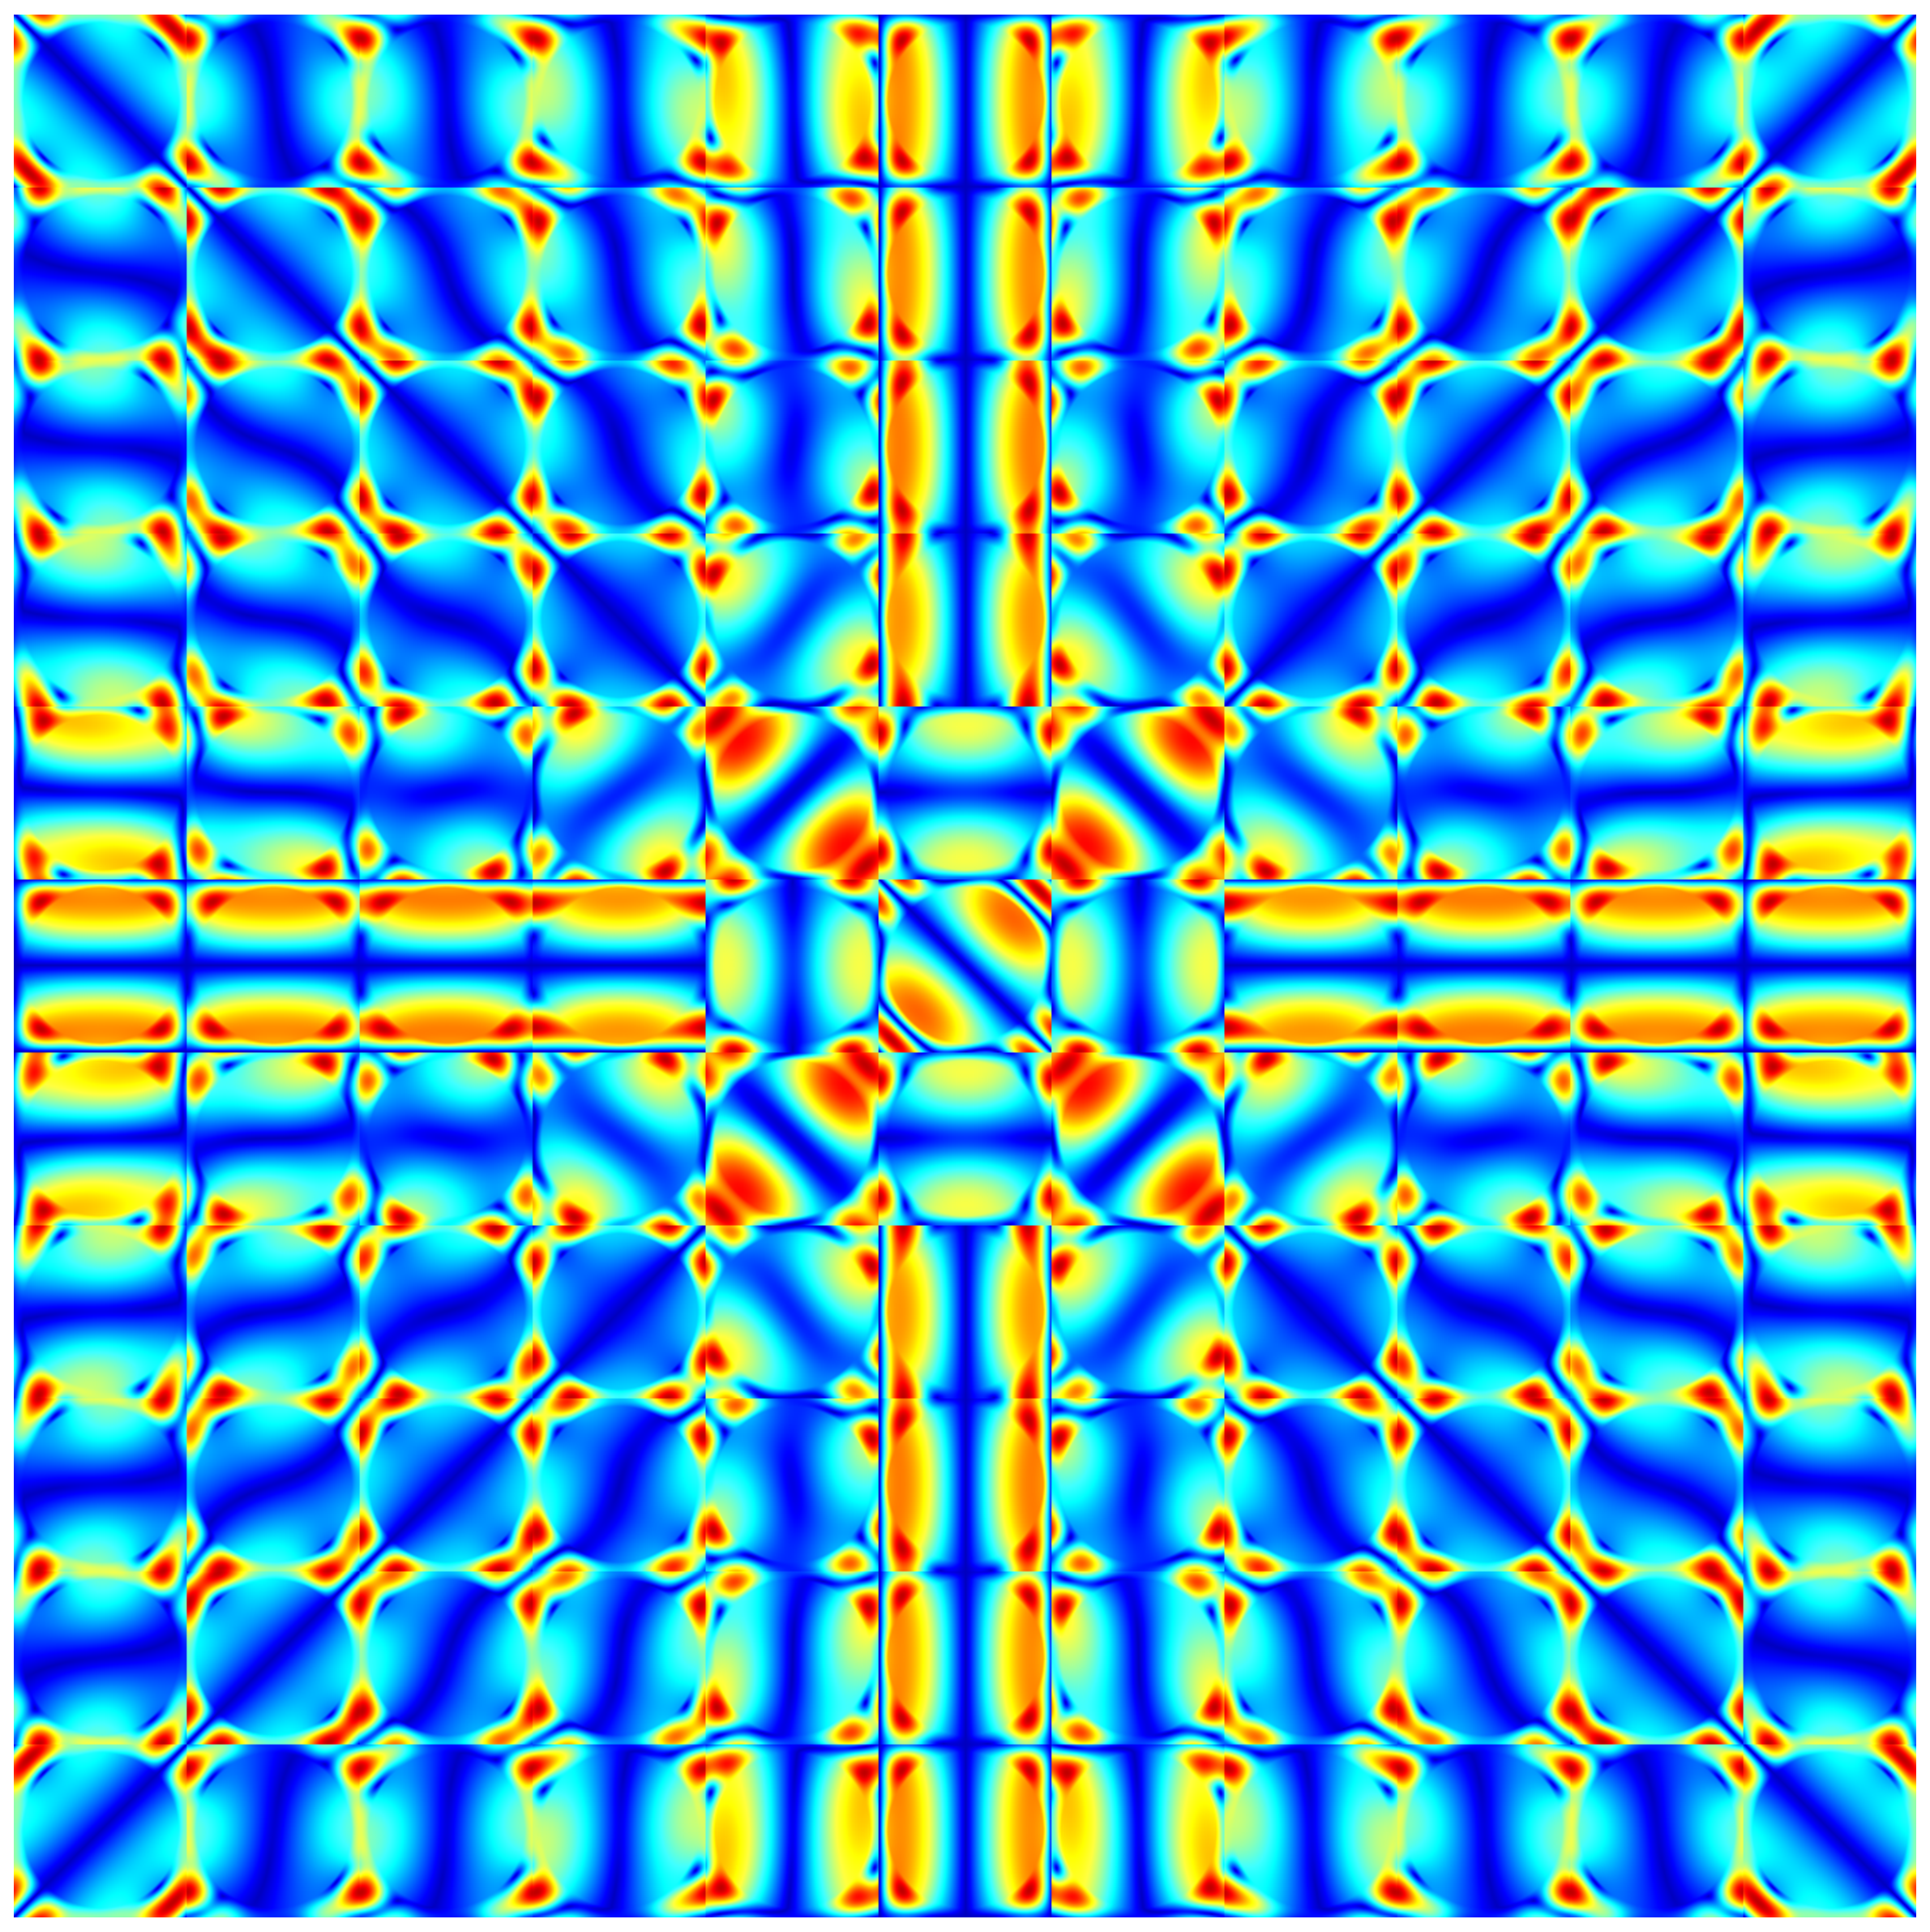
\includegraphics[width=9cm]{Titlepage/coverpicture.eps}\\
    }
    \vspace*{\stretch{8}}
    { \Large
      \color{red} Bachelor's/Master's thesis \\
      \vspace*{\stretch{0.5}}
      by \\
      \vspace*{\stretch{0.5}}
      \bf \color{red} author \\
    }
    \vspace*{\stretch{2}}
    { \large 
      \color{red} hand-in date\\
    }
    \vspace*{\stretch{5}}
    { \large
      \begin{tabular}{r@{\hspace{2em}}l}
        Instructor:     & Prof.~Dr.~J"org Schmalian\\
        2nd Instructor: & PD.~Igor~Gornyi
      \end{tabular}
    }
  \end{center}
  \vspace*{\stretch{1}}
\end{titlepage}
\cleardoublepage
 %%% if the thesis is english, add a second english titlepage
%\chapter{Acknowledgments}

I would like to express my thanks to my advisor J\"org Schmalian who encouraged and supported me and gave the right hints at the right time during the last year. 
His essential input lead to the results presented in this work. 

Furthermore, I would like to thank Una Karahasanovic for all the discussions and information which became decisive for one topic of this work. 

Then, I have to thank especially Jian Kang who crucially contributed to the discussion of bond currents and Rafael Fernandes for the fruitful discussions on the general topic. 

Special thanks to all the colleagues of the condensed matter group at the KIT. Especially to Bhilahari Jeevanesan for all the discussions and help with several problems and to Pablo Schad for finalizing this work. 

Last but not least, I have to thank my family, my mother and sister and especially Anja for all the support and encouraging words. 
 
   %%% acknowledge help from colleagues and friends 

\tableofcontents %Inhaltsverzeichnis
%\listoffigures

\pagestyle{scrheadings}			%%% for normal text, display section names in header line

\mainmatter
%%Modify overview chapter
\makeatletter% siehe De-TeX-FAQ
\renewcommand*{\chapterformat}{%
\begingroup% damit \unitlength-Änderung lokal bleibt
\setlength{\unitlength}{1mm}%
\begin{picture}(0,40)(0,5)%
\setlength{\fboxsep}{0pt}%
%\put(0,0){\framebox(20,30){}}%
%\put(0,20){\makebox(20,20){\rule{20\unitlength}{20\unitlength}}}%
\put(0,15){\color{black}\linethickness{0.4pt}\line(1,0){\dimexpr\textwidth-0\unitlength\relax\@gobble}}% line
%\put(0,0){\makebox(18,20)[r]{\fontsize{20\unitlength}{1}\color{white}\selectfont\thechapter %\kern-.04em% Ziffer in der Zeichenzelle nach rechts schieben
%}}%
\put(20,15){\makebox(\dimexpr \textwidth-20\unitlength\relax\@gobble,\ht\strutbox\@gobble)[l]{%\ %\normalsize\color{black}\chapapp~\thechapter\autodot 
}}%
\end{picture} % <- Leerzeichen ist hier beabsichtigt!
\endgroup
}%
\makeatother

\newcommand{\nocontentsline}[3]{}
\newcommand{\tocless}[2]{\bgroup\let\addcontentsline=\nocontentsline#1{#2}\egroup}

\setcounter{chapter}{-1}
\tocless\chapter{Overview}
\addcontentsline{toc}{chapter}{Overview}


%%%%%%%%%%%%%%%%%%%%%%%%%%%%%%%%%%%%%%%%%%%%%%%%%%%%%%%%%%%%%
%%%%%%%%%%%%%%%%%%%%%%%%%%%%%%%%%%%%%%%%%%%%%%%%%%%%%%%%%%%%
%%%%%%%                            %%%%%%%%%%%%%%%%%%%%%%%%%
%%%%%   chapter headings             %%%%%%%%%%%%%%%%%%%%%%%
%%%%%%                             %%%%%%%%%%%%%%%%%%%%%%%%%
%%%%%%%%%%%%%%%%%%%%%%%%%%%%%%%%%%%%%%%%%%%%%%%%%%%%%%%%%%%%
%%%%%%%%%%%%%%%%%%%%%%%%%%%%%%%%%%%%%%%%%%%%%%%%%%%%%%%%%%%%

%%% INFO: when using different fonts, the chapter headings may look
%%% different and the given sizes do no longer apply!

\colorlet{chapter}{darkblue}
\addtokomafont{chapter}{\color{black}}

\makeatletter% siehe De-TeX-FAQ
\renewcommand*{\chapterformat}{%
\begingroup% damit \unitlength-Änderung lokal bleibt
\setlength{\unitlength}{1mm}%
\begin{picture}(20,40)(0,5)%
\setlength{\fboxsep}{0pt}%
%\put(0,0){\framebox(20,30){}}%
%\put(0,20){\makebox(20,20){\rule{20\unitlength}{20\unitlength}}}%
\put(20,15){\color{black}\linethickness{0.4pt}\line(1,0){\dimexpr\textwidth-20\unitlength\relax\@gobble}}% line
\put(0,0){\makebox(18,20)[r]{\fontsize{20\unitlength}{1}\color{black}\selectfont\thechapter %\kern-.04em% Ziffer in der Zeichenzelle nach rechts schieben
}}%
\put(20,15){\makebox(\dimexpr \textwidth-20\unitlength\relax\@gobble,\ht\strutbox\@gobble)[l]{%\ %\normalsize\color{black}\chapapp~\thechapter\autodot 
}}%
\end{picture} % <- Leerzeichen ist hier beabsichtigt!
\endgroup
}%
\makeatother


\chapter{Introduction}
\label{ch:introduction}

% Zun\"achst: transport in graphene, warum cool
First successfull transport experiments in graphene \cite{Zhang2005}, \cite{Novoselov2005}

First thing that is weird about (gapless) graphene: it is described by a relativistic, massless Dirac electrons. Experiments \cite{Novoselov2005} show that electronic transport is goverened by Dirac equation, charge carriers have an effective "speed of light". This paper shows unusual effects that are characteristic for two-dimensional Dirac fermions: 1) Conductivity in graphene never falls below a minimum value (even when charge carrier density goes to zero) 2) anomalous integer quantum hall effect (occurs at half integer filling factors)
Transport measurements in graphene: integer quantum hall effect, weak localization, 

\cite{Zhu2017}: Spectra of MLG and BLG graphene are gapless and protected by symmetry of crystal lattice. When symmetry is broken by interaction with substrate or applying electric field: energy gap opens. In BLG: energy gap can be controlled by displacement field $\mathbf{D}$. Controlled induction of insulating state in graphene \cite{Oostinga2008}

\cite{Zhu2017}: Manchester group, proximity induces superconductivity: high gap energies (big gap), but still there is low resistivity (not the expected insulating state). Conductive channels were found an explained for both MLG and BLG at the Charge neutrality point and were explained by valley currents, zero energy edge states. 

supercurrent at charge neutrality point porpagates along edge channels, shunts the insulating bulk in graphene. Question adressed: in graphene, large gaps can be opened, but they rarely lead to an highly insulating state which would be expected at low temperatures. Idea: edge currents are responsible for transport, edge conductance due to nontrivial topology of gapped Dirac spectrum: 1) electronic states due to zigzag segments. 2) valley Hall effect ?
%Übergang zu Supraleitung und Fraunhofer paatern

Why study Fraunhofer patterns? By measuring critical current as a function of perpendicular B, the local current density in x direction perpendicular to current flow can be deduced \cite{Dynes1971}. By variying top and bottom voltage it is possible to keep BLG graphene charge neutral while doping the two graphene layers with the opposite sign. This results into the displacement field which translates directly into the gap.At high doping ($E_F > E_\text{gap}$, the critical current depends weakly on the displacement field.

\cite{Heersche2007}: Josephson effect in mesoscopic junctions: charge density in the graphene layer can be controlled by a gate electrode. Observation of of a supercurrent that (depending on gate voltage) is carried either by electrons in the conduction band or by holes in the valence band. finding of a finite normal state conductance and finite supercurrent at zero charge density

%Zusammenfassung: supercurrent ist geil und kann genutzt werden, um den Stromfluss zu untersuchen. Aber die Frage  ist doch eigentlich: kann man die Amplitude und das confinement gleichzeitig ver\"andern? Siehe dazu das QPC gate!


\chapter{Framework for analytical model}
\label{ch:basics}

\section{Theory of superconductivity}

The discovery of the isotope effect in 1950 revealed that not only lattice electrons but rather the whole lattice determines the superconducting properties of a solid. Experiments measuring the critical temperature $T_c$ of different mercury isotopes showed that indeed, there is a relation between the isotope mass and $T_c$. Herbert Fr\"olich was then the first to introduce a new concept to explain superconductivity. He showed that a phonon-intermediated interaction between electrons and the lattice could lead to an attractive long-range interaction of electrons in the lattice. Figuratively speaking, an electron passing through the crystal lattice will polarize it by attracting the positive ions. It leaves a deformed lattice, which will then attract a second electron. An effective attractive interaction between these two electrons is created. % – they form a Cooper pair. 
In 1956, Cooper showed that the electronic ground state, the Fermi sea at $T = 0$, is unstable if a weak attractive interaction is taken into account. This layed the foundation of the BCS theory \cite{Bardeen1957}, the first microscopic theory after the discovery in 1911 by Heike Kammerlingh Onnes. 

%TODO maybe include picture that explains, why opposite k vectors

\subsection*{Formulas needed}
Hamiltonian:
\begin{align}
H &= H_0 + H_1 \label{eq:H}\\
H_0 &= \sum_{\mathbf{k}, \sigma} \xi_{\mathbf{k}} c^{\dagger}_{\mathbf{k} \sigma }c_{\mathbf{k} \sigma }  \label{eq:H0}\\
H_1 &= \frac{1}{N} \sum_{\mathbf{k}, \mathbf{k'}} V_\mathbf{{\mathbf{k}, \mathbf{k'}}} c^{\dagger}_{\mathbf{k} \uparrow }c^{\dagger}_{- \mathbf{k} \downarrow}   c_{- \mathbf{k'} \downarrow} c_{\mathbf{k'} \uparrow} \label{eq:H1}
\end{align}
The operators $c^\dagger_{\mathbf{k}, \sigma} , c_{\mathbf{k}, \sigma}$ are fermion operators that create or annihilate an electron with momentum $\mathbf{k}$ and spin $\sigma$. The first term in the Hamiltonian $H$ is the unperturbed electron Hamiltonian $H_0$ with parabolic energy dispersion $\xi_{\mathbf{k}}$. The  second term is the interaction Hamiltonian $H_1$, expressing the scattering of two electrons from $(- \mathbf{k'} \downarrow,  \mathbf{k'} \uparrow)$ to $(\mathbf{k} \uparrow , - \mathbf{k} \downarrow)$. The interaction potential $V_\mathbf{{\mathbf{k}, \mathbf{k'}}}$ exchanges the scattering for electrons with energy $|\xi_\mathbf{k}| \lesssim \hbar \omega_D$.
%TODO check!
The Hamiltonian in eq. (\ref{eq:H}) can be simplified by doing a mean-field approximation. In this approximation, an operator $A$ is expressed by a sum of its statistical mean $\braket{A}$ and small statistical fluctuations $\delta A$. Since the fluctuations are assumed to be small, terms with $\mathcal{O}((\delta A)^2)$ can be neglected.
\begin{align}
A &= \langle A \rangle + \delta A, \quad B = \langle B \rangle + \delta B  \nonumber \\
A B &= \langle A \rangle  \langle B \rangle  + \langle A \rangle  \delta B +  \langle B \rangle \delta A + \underbrace{\delta A \delta B}_{\approx 0}\label{eq:meanfield-der}
\end{align}
Using $\delta A = A - \langle A \rangle$ and inserting this back into eq. (\ref{eq:meanfield-der}) leads to
\begin{equation}
AB = \langle A \rangle B + \langle B \rangle A - \langle A \rangle \langle B \rangle.\label{eq:meanfield-ab}
\end{equation}
This approximation is applied to the interaction part $H_1$ in eq. (\ref{eq:H1}), replacing
\begin{equation}
A = c^{\dagger}_{\mathbf{k} \uparrow }c^{\dagger}_{- \mathbf{k} \downarrow}, \quad B =  c_{- \mathbf{k'} \downarrow} c_{\mathbf{k'} \uparrow} .
\end{equation}
The result is the BCS-Hamiltonian
\begin{equation}
H_{\text{BCS}} = \sum_{\mathbf{k}, \sigma} \xi_{\mathbf{k}} c^{\dagger}_{\mathbf{k} \sigma }c_{\mathbf{k} \sigma }    -  \sum_{\mathbf{k}} \Delta_{\mathbf{k}}^* c_{-\mathbf{k}, \downarrow} c_{\mathbf{k}, \uparrow}  - \sum_{\mathbf{k}} \Delta_{\mathbf{k}}  c^{\dagger}_{\mathbf{k} \uparrow} c^{\dagger}_{- \mathbf{k} \downarrow} + \text{const.}\label{eq:H-BCS}
\end{equation}
where 
\begin{eqnarray}
\Delta_{\mathbf{k}} &:=& - \frac{1}{N} \sum_{\mathbf{k'}} V_\mathbf{{\mathbf{k} \mathbf{k'}}} \langle c_{-\mathbf{k'}, \downarrow} c_{\mathbf{k'} \uparrow} \rangle \\
\Delta_{\mathbf{k}}^* &:=& - \frac{1}{N} \sum_{\mathbf{k'}} V_\mathbf{{\mathbf{k}, \mathbf{k'}}}  \langle  c^{\dagger}_{\mathbf{k'} \uparrow} c^{\dagger}_{- \mathbf{k'} \downarrow} \rangle
\end{eqnarray}
%TODO why is this the pair potential?
The BCS-Hamiltonian in eq. (\ref{eq:H-BCS}) can be diagonalized using the Bogoliubov transformation. The aim is to express the Hamiltonian in the basis of new fermion operators. These new operators will describe quasiparticles, which are a linear combination of $c^\dagger_{\mathbf{k}, \sigma}$ and $c_{\mathbf{k}, \sigma}$.
\begin{equation}
\begin{pmatrix}
\gamma_{\mathbf{k} \uparrow} \\ \gamma^{\dagger}_{-\mathbf{k} \downarrow}  
\end{pmatrix} = \begin{pmatrix}
u^*_{\mathbf{k} } & -v_{\mathbf{k} } \\
v^*_{\mathbf{k} }  & u_{\mathbf{k} } 
\end{pmatrix} 
\begin{pmatrix}
c_{\mathbf{k} \uparrow} \\ c^{\dagger}_{-\mathbf{k} \downarrow}  
\end{pmatrix}
\end{equation}\label{eq:bogol-trans}
Evaluating the fermion anticommutation relation using the transformation above yields
\begin{equation}
\left\{ \gamma_{\mathbf{k} \uparrow}, \gamma^{\dagger}_{\mathbf{k} \uparrow}  \right\}  = \dots = |u_{\mathbf{k}}|^2 | + v_{\mathbf{k}}|^2 \stackrel{!}{=} 1
\end{equation}
and will lead to the inverse transformation of eq. (\ref{eq:bogol-trans}). Inserting the inverse transformation into the BCS-Hamiltonian in eq.(\ref{eq:H-BCS}) will give the coefficients $u_{\mathbf{k}}$, $v_{\mathbf{k}}$ from eq. (\ref{eq:bogol-trans}) and finally yield to the diagonalized form of the BCS-Hamiltonian
\begin{eqnarray}
H_{\text{BCS}} &=&  \sum_{ \mathbf{k} \sigma } E_{ \mathbf{k} } \gamma^{\dagger}_{\mathbf{k} \sigma } \gamma_{\mathbf{k} \sigma }\\
E_{\mathbf{k}} &:=&  \sqrt{\xi^2_{\mathbf{k}}  + |\Delta_{\mathbf{k}}|^2 } \label{eq:E-k}
\end{eqnarray}
\begin{figure}
\centering
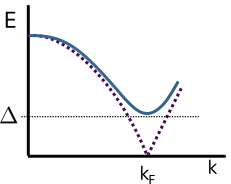
\includegraphics[width=0.5\textwidth]{figure/framework-analytical/bcs-spectrum}
\caption{Excitations from BCS theory. The dashed line is the normal state dispersion relation ($\Delta = 0$). The solid line is the dispersion relation for the superconducting state ($\Delta \neq 0$), where no excitations with energies $\epsilon < \Delta$ are present. } \label{fig:bcs-spectrum}
\end{figure}
For a fixed energy $E_k$, eq. (\ref{eq:E-k}) gives two possible values for $\xi_k$:
\begin{equation}
\xi_k = \pm \sqrt{\epsilon^2 - | \Delta_k|^2}.
\end{equation}
Knowing that $k^2 = k_F^2 \pm 2m\sqrt{\epsilon^2 + |Delta_k|^2} \hbar^2$, one can calculate the group velocity as 
\begin{equation}
v_g = \frac{d \epsilon}{d (\hbar k)} = \pm v_F \frac{\sqrt{\epsilon^2 - |\Delta|^2}}{\epsilon}.
\end{equation}
The group velocity is positive for excitations outside the Fermi surface and negative for excitations inside. Therefore, the positive solution is a particle-like excitation, and the negative solution is a hole-like excitation. Figure \ref{fig:bcs-spectrum} shows the excitation spectrum of particles and holes from the BCS theory. 

\subsection*{Bogoliubov de Gennes Hamiltonian}
%Motivation for BdG: Describing inhomogneous systems, example Josephson junctions --> need for a microsopic theory for inhomogenous systems. 
%Idea: make BCS- mean field hamiltonian spatially dependent. 
The ansatz for the BCS ground state used by Bardeen, Cooper and Schrieffer is based on the concept of Cooper pairs. It is a direct consequence of the instability in the ground state through the attractive interaction. The BCS theory proposes a BCS ground state built on eigenstates of the single-particle Hamiltonian $H_0$ from eq. (\ref{eq:H0}), leading to a ground state that consists of a linear combination of pair states. %TODO check!
\begin{eqnarray}
\ket{\psi_\text{BCS}} &=& \prod_{ \mathbf{k} } (u_\mathbf{k} + v_\mathbf{k} c^{\dagger}_{ \mathbf{k} \uparrow } c^{\dagger}_{ - \mathbf{k} \downarrow }) \ket{\text{vac}} \\
H_\text{BCS} \ket{\psi_\text{BCS}} &=& E_\text{BCS} \ket{\psi_\text{BCS}}  
\end{eqnarray}
In most cases however, a more realistic set-up or inhomogeneous system cannot be described in terms of eigenfunctions of $H_0$. With a vector potential $\mathbf{A} \neq 0$, for example, time reversal symmetry is not given any more. %TODO Überleitung (“In the general case”)
The characteristic length scale is the superconducting coherence length $\xi_0$. If a system is varying slowly over a length scale $l \approx \xi_0$, a spatially dependent, more general Hamiltonian is needed. 
In order to find an adequate expression for such a spatially dependent Hamiltonian, the following spinor is introduced
\begin{equation}
\ket{\Psi_\mathbf{k}} = \begin{pmatrix}
| \Psi_\mathbf{k_1} \rangle \\ | \Psi_\mathbf{k_2} \rangle
\end{pmatrix} := \begin{pmatrix}
c^{\dagger}_{\mathbf{k}, \uparrow} \\ c_{- \mathbf{k}, \downarrow}
\end{pmatrix} \ket{\psi_\text{BCS}} \label{eq:spinor}
\end{equation}
In this basis $\left\{| \Psi_\mathbf{k_1} \rangle, | \Psi_\mathbf{k_2} \rangle \right\}$, the Hamiltonian is (and this is the Bogoliubov de Gennes Hamiltonian with energies relative to $E_\mathbf{k}$):
\begin{equation}
H_\text{BdG}\left(\mathbf{k} \right) = \begin{pmatrix}
\xi_\mathbf{k} &  - \Delta_\mathbf{k}\\
- \Delta^*_\mathbf{k} & - \xi_\mathbf{k}
\end{pmatrix} \label{eq:H-BdG}
\end{equation}
%For this, the commutation relation for $H_\text{BCS}$ and $c^\dagger_{\mathbf{k}, \uparrow}$, $c_{- \mathbf{k}, \downarrow}$ have been used.
This Hamiltonian form eq. (\ref{eq:H-BdG}) has the eigenvalues
\begin{equation}
 \pm E_\mathbf{k} = \pm \sqrt{\xi_\mathbf{k}^2 + |\Delta_\mathbf{k}|^2  }.
\end{equation}
%Include eigenstates?
To finally arrive at the spatially dependent form of eg. (\ref{eq:H-BdG}), the Hamiltonian is Fourier-transformed.
\begin{eqnarray}
H_\text{BdG} \left( \mathbf{r} \right) &:=& \frac{1}{N} \sum_\mathbf{k} e^{i \mathbf{k \cdot r}} H_\text{BdG}\left( \mathbf{k} \right) \\
&=& \begin{pmatrix}
H_0\left( \mathbf{r} \right)  &  - \Delta \left( \mathbf{r} \right) \\
- \Delta^* \left( \mathbf{r} \right)  & - H_0 \left( \mathbf{r} \right) 
\end{pmatrix} \label{eq:H-BdG-r}
\end{eqnarray}
$H_0 \left( \mathbf{r} \right) $ is the free Hamiltonian. Corresponding Schr\"odinger equaions are called BdG-equations:
\begin{eqnarray}
H_\text{BdG} \left( \mathbf{r} \right) \Psi\left( \mathbf{r} \right) &=& E \Psi\left( \mathbf{r} \right)\label{eq:BdG-eq} \\
\Psi\left( \mathbf{r} \right)  &=& \begin{pmatrix}
\Psi_1\left( \mathbf{r} \right) \\ \Psi_2\left( \mathbf{r} \right) 
\end{pmatrix}\label{eq:BdG-spinor}
\end{eqnarray}

\section{Andreev reflection- NS interface}\label{sec:NS}

Now that the principles of BCS theory have been established, the physical effects at the interface between a superconductor and a normal are to be outlined.\\
The most important detail when modelling the interface between a superconductor and a normal metal is the superconducting order parameter $\Delta \left( \mathbf{r} \right)$. It is present in the superconducting region and zero in a normal metal. To keep the model as simple as possible, a step-like behaviour is assumed. This means that for an interface placed at $x=0$, the superconducting order parameter becomes a function of $x$ and can be written as
\begin{equation}
\Delta \left( x \right) = \theta \left(x \right).\label{eq:delta }
\end{equation}
\begin{figure}
\centering
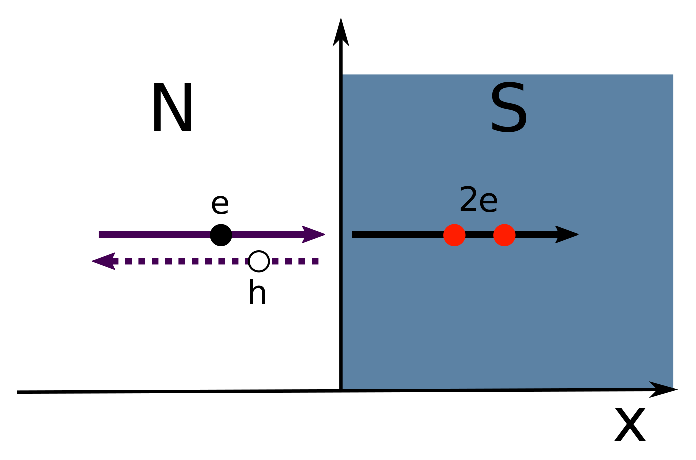
\includegraphics[width=0.5\textwidth]{figure/framework-analytical/ns-interface}
\caption{Andreev reflection at an NS interface. An incoming electron is Andreev reflected into a hole with opposite momentum, and a Cooper pair condensates into the superconductor. The interface is modelled as a sharp edge.}\label{fig:ns-interface}
\end{figure}
How does this model differ from a quantum mechanical step potential set-up? The formalism is virtually identical, but there is a subtle and important difference in the results. In the normal region, there are electrons, whereas in the superconducting regions, there is a condensate of Cooper pairs. A normal electron can be reflected at the interface as a hole and an additional Cooper pair can be created in the superconducting region (see figure \ref{fig:ns-interface}). By solving the Bogoliubov-de-Gennes equation in (\ref{eq:BdG-eq}), this picture becomes clearer.  This equation needs to be solved both for the normal and the superconducting region. When treating this problem quantum-mechanically, energies below and above the gap need to be considered independently. The resulting wave functions have to be continuous at the interface. Depending on the region, the gap parameter in the Hamiltonian in eq. (\ref{eq:H-BdG-r}) is either zero or $\Delta_0$.

\subsection*{Semi-classical approximation: Andreev equations}

In case of the NS interface, the gap parameter varies slowly over scales of $k_F$, and it may vary over scales of the coherence length $\xi_0$. Because $k_F$ is a good length scale for this problem, the equations above can be simplified:
\begin{equation}
\Psi \left( \mathbf{r} \right) = e^{i \mathbf{k_F} \mathbf{r} } \begin{pmatrix} u \left( \mathbf{r} \right) \\ v \left( \mathbf{r} \right)\end{pmatrix}.
\end{equation}
Since $u  \left( \mathbf{r} \right) $ and $v  \left( \mathbf{r} \right) $ vary slowly over distances of order $k_F^{-1}$, the second derivative can be neglected. This is the semi-classical approximation, which then leads to the Andreev equations
\begin{eqnarray}
- i \hbar \mathbf{v}_F \nabla u \left( \mathbf{r} \right)  + \Delta \left( \mathbf{r} \right)  v  \left( \mathbf{r} \right)  &=& \epsilon u  \left( \mathbf{r} \right)  \\
 i \hbar \mathbf{v}_F \nabla v  \left( \mathbf{r} \right)  + \Delta^* \left( \mathbf{r} \right)  u  \left( \mathbf{r} \right)  &=& \epsilon v  \left( \mathbf{r} \right) .
\end{eqnarray}
These equations are significantly easier to handle than the BdG-equations, since they describe a first-order problem.
\newline
\newline
Consider an incoming particle from the left half-space $x < 0 $, travelling towards the superconducting interface at $x=0$, assuming that both the normal region and the superconductor have the same Fermi velocity $k_F^{-1}$. The one-dimensional Andreev equations for the NS interface read
\begin{eqnarray}
- i \hbar v_{F, x} \frac{d}{d x} u \left( x \right)  + \Delta(x) v \left( x \right) &=& \epsilon u \left( x \right)\\
 i \hbar v_{F, x} \frac{d}{d x} v \left( x \right) + \Delta^*(x) u \left( x \right) &=& \epsilon v \left( x \right).
\end{eqnarray}
%\subsubsection*{Solution for the normal region}
In the normal region (for $x < 0$) the superconducting gap parameter decreases to zero on a length scale shorter than $\xi$. Therefore, the step-like approximation from eq. (\ref{eq:delta }) holds. In the normal region, 
the coefficients $u \left( x \right)$ and $v \left( x \right)$ are independent. The ansatz contains an incident wave with unity amplitude and a reflected hole with amplitude $r$. 
\begin{equation}
\Psi_N \left( x \right) = \begin{pmatrix} u \left( x \right) \\ v \left( x \right) \end{pmatrix}_N = e^{i k_N x } \begin{pmatrix} 1 \\ 0 \end{pmatrix} + r e^{-i k_N x } \begin{pmatrix} 0 \\ 1 \end{pmatrix}  \label{eq:psi-normal}
\end{equation}
where, writing $v_x \equiv v_{F, x}$, 
\begin{equation}
k_N = \frac{\epsilon}{\hbar v_x}
\end{equation}
%TODO den Teil da unten wieder reinnehmen, wenn verstanden?
%\subsubsection*{Solution in the superconducting region}
In the superconducting region, the solution for the wave function has the form
\begin{equation}
\Psi_S \left( x \right) = \begin{pmatrix} u \left( x \right) \\ v \left( x \right) \end{pmatrix}_S = t e^{i k_S x } \begin{pmatrix} u_0 \\ v_0 \end{pmatrix}.
\end{equation}
The expression for the wave vector $k_S$ depends on the energy of the incoming particle, which can be either \emph{above} or \emph{below} the gap.\newline \newline
For high energies \emph{above} the gap,  $\epsilon > |\Delta|$ , the wave vector is
\begin{equation}
k_S = \frac{\sqrt{\epsilon^2 - \Delta^2}}{\hbar v_x}
\end{equation}
If the energy of the incoming particle is higher than the gap energy, it can be transmitted into the superconductor. The amplitude $t$ therefore is the transmission probability. The coherence factors $u_0$, $v_0$ can be found by solving the BdG equations within the BCS framework. Matching the boundary conditions at the interface yields
\begin{equation}
r = \frac{v_0}{u_0}, \quad t = \frac{1}{u_0}.
\end{equation}
Normalizing the wave functions leads to 
\begin{equation}
|r|^2 + (u_0^2 - v_0^2)|t|^2 = 1
\end{equation}
Since $\epsilon$ is the energy relative to the Fermi energy, the normal wave vector from eq. (\ref{eq:psi-normal}) can be written in terms of
\begin{equation}
\mathbf{q}_\pm =  \left( k_F \pm \frac{\epsilon}{\hbar v_F} \right) \hat{\mathbf{k}_F} \label{eq:q-pm}
\end{equation}
\begin{equation}
\Psi_N \left( \mathbf{r} \right) = e^{i\mathbf{q}_+ \cdot \mathbf{r}} \begin{pmatrix} 1 \\ 0\end{pmatrix} + a e^{i\mathbf{q}_- \cdot \mathbf{r}} \begin{pmatrix} 0 \\ 1\end{pmatrix},
\end{equation}
Using eq. (\ref{eq:q-pm}), one finds the trajectory of the reflected hole to coincide with the trajectory of the incoming electron. The change in momentum,
\begin{equation}
\Delta p_x = - \frac{2 e }{v_x},
\end{equation}
$\Delta p_x$ is small. The components $p_y$, $p_z$ are conserved, therefore the trajectory of the reflected hole is almost the same as the trajectory of the incoming electron. %TODO figure!
%In this solution, the incoming electron has the momentum 
%\begin{equation}
%q  = k_F + \frac{\epsilon}{\hbar v_F} \quad \rightarrow \epsilon(q) = \hbar v_F \left( q - k_F \right)
%\end{equation}
%with a positive group velocity $v_g = v_F$, whereas the reflected hole has the momentum
%\begin{equation}
%q  = k_F - \frac{\epsilon}{\hbar v_F} \quad \rightarrow \epsilon(q) = \hbar v_F \left( k_F - q \right)
%\end{equation} 
%with negative group velocity $v_g = - v_F$. \\
\newline
\newline
For energies \emph{below} the gap, $\epsilon < |\Delta |$, there are no states available inside the gap, therefore the wave function decays inside the superconductor. 
\begin{equation}
\tilde{k}_S= \frac{\sqrt{\Delta^2 - \epsilon^2 }}{\hbar v_x}.
\end{equation}
The wave function is
\begin{equation}
\begin{pmatrix} u\left(x\right) \\ v\left(x\right) \end{pmatrix}_S = t e^{- \tilde{k_S} x } \begin{pmatrix} u_0 \\ v_0 \end{pmatrix}.
\end{equation}
For sub-gap energies, the amplitudes of the normal wave functions are slightly modified:
\begin{equation}
r = \frac{\tilde{v_0}}{\tilde{u_0}}, \quad t = \frac{1}{\tilde{u_0}}
\end{equation}
and 
\begin{equation}
\tilde{u_0} = \frac{1}{\sqrt{2}} \left( 1 + i \frac{\sqrt{|\Delta|^2 - \epsilon^2}}{\epsilon} \right), \quad \tilde{v_0} = \frac{1}{\sqrt{2}} \left( 1 - i \frac{\sqrt{|\Delta|^2 - \epsilon^2}}{\epsilon} \right).
\end{equation}
In this case, it holds that
\begin{equation}
|a|^2 = 1
\end{equation}
In other words, there are no transmitted particles and all particles are Andreev reflected.

\section{Theory of SNS junction}\label{sec:theory-sns}
So far, only NS interfaces have been considered. The same procedure can be applied to superconductor - normal metal - superconductor (SNS) junctions: A sandwich structure of a superconductor on the left side, a normal region in the middle and a superconductor on the right side. At both interfaces, a particle can be Andreev-reflected.
Each time an electron is Andreev reflected at the right side and a hole travels back, a cooper pair is induced into the right superconductor. In the same manner, a cooper pair is stolen from the left superconductor when the hole is Andreev reflected as an electron. This process is illustrated in figure \ref{fig:sns-junction}. As an overall consequence, a supercurrent through the SNS junction can be observed. This process leads to localized electrons with bound states, the so called Andreev bound states. \\

\begin{figure}
\centering
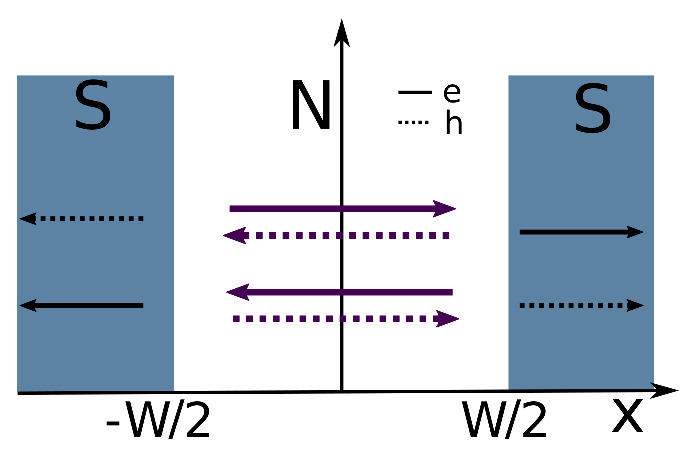
\includegraphics[width=0.5\textwidth]{figure/framework-analytical/sns}
\caption{A SNS junction with width $W$. Electrons are indicated as solid arrow, holes as dashed ones. An electron (hole) is Andreev reflected as a hole (electron) at one side, which then again is reflected at the other side. In this way, Andreev bound states form in the junction.}\label{fig:sns-junction}
\end{figure}
A SNS junction with normal region at $|x| < W/2$, the right superconductor at $x > + W/2$ and the left superconductor at $x < -W/2$ is considered. The electrons in both superconducting regions and in the normal metal have the same Fermi velocity and there are no insulating barriers between them. This means that $W$  is smaller than the electron mean free path. For short $W$ this implies that the mean free path is larger than the superconducting coherence length (?). The phase difference between the superconductors is $\chi$, so the right supercondctor has phase $\chi/2$ and the left has $-\chi/2$. 
The semi classical approximation is used and a wave function with the form
\begin{equation}
\Psi \left( \mathbf{r} \right) = e^{i \mathbf{k_F} \mathbf{r} } \begin{pmatrix} u \left( \mathbf{r} \right) \\ v \left( \mathbf{r} \right)\end{pmatrix}.
\end{equation}
is needed. 
In the normal region, it holds that 
\begin{eqnarray}
\Psi_N \left( x \right) &=& A\cdot \left[ e^{i k_N x } \begin{pmatrix} 1 \\ 0 \end{pmatrix} + a e^{-i k_N x } \begin{pmatrix} 0 \\ 1 \end{pmatrix} \right], \label{eq:sns-psi-normal}\\
k_N &=& \frac{\epsilon}{\hbar v_x}.
\end{eqnarray}
Assuming that $k_x > 0$, the wave function in the right superconductor ($x > W/2$) is
%\begin{pmatrix} u \left( x \right) \\ v \left( x \right) \end{pmatrix}_R 
\begin{eqnarray}
\Psi_S^R \left( x \right) &=& d_1 e^{ - \tilde{k}_S x } \begin{pmatrix} \tilde{u}_0 e^{i \chi/4} \\ \tilde{v}_0 e^{-i \chi/4} \end{pmatrix},\\
\tilde{k}_S  &=& \frac{\sqrt{|\Delta|^2 - \epsilon^2 }}{\hbar |v_x|}.
\end{eqnarray}
For the left superconductor, the wave function is
\begin{equation}
 \Psi_S^L \left( x \right) = d_1' e^{ \tilde{k}_S x } \begin{pmatrix} \tilde{v}_0 e^{-i \chi / 4}\\ \tilde{u}_0 e^{i \chi / 4} \end{pmatrix}.
\end{equation}
Applying the continuity condition at the interfaces leads to
\begin{eqnarray}
a e^{-i k_n W} &=& \frac{\tilde{v}_0}{\tilde{u}_0} e^{-i \chi /2}  \\
a e^{i k_n W} &=& \frac{\tilde{u}_0}{\tilde{v}_0} e^{i \chi /2}.
\end{eqnarray}
Combining these equations, we find
\begin{equation}
e^{2i ( k_N W - \chi /2 )}  = \frac{\epsilon + i \sqrt{|\Delta|^2 - \epsilon^2 }}{ \epsilon - i \sqrt{|\Delta|^2 - \epsilon^2 } } \label{eq:energy-exp}.
\end{equation}
To simplify this expression, one can introduce 
\begin{equation}
\sin \alpha := \frac{\epsilon}{|\Delta|}, \quad - \pi / 2 < \alpha < \pi / 2\label{eq:sinalpha}
\end{equation}
Using eq. (\ref{eq:sinalpha}), one can rewrite the right hand side of eq. (\ref{eq:energy-exp}) in terms of trigonometric functions and gets
\begin{equation}
e^{2i ( k_N W - \chi /2 )} = e^{-2i \alpha + i \pi},
\end{equation}
which then leads to
\begin{equation}
\epsilon = \frac{\hbar v_x}{W} \left( \pi \left(l + \frac{1}{2} \right) - \arcsin \frac{\epsilon}{|\Delta|} + \frac{\chi}{2} \right).
\end{equation}
%TODO short summary, what has been done up to this point?
If $k_x < 0 $, it holds that
\begin{equation}
\Psi_S^R \left( x \right) = d_2 e^{ - \tilde{k}_S x } \begin{pmatrix} \tilde{v}_0 e^{i \chi/4} \\ \tilde{u}_0 e^{-i \chi/4} \end{pmatrix}
\end{equation}
For the left superconductor, the wave function is
\begin{equation}
\Psi_S^L \left( x \right)  = d_2' e^{ \tilde{k}_S x } \begin{pmatrix} \tilde{u}_0 e^{-i \chi / 4}\\ \tilde{v}_0 e^{i \chi / 4} \end{pmatrix}
\end{equation}
An analogous calculation leads to
\begin{equation}
\epsilon = - \frac{\hbar |v_x|}{W} \left( \pi \left(l - \frac{1}{2} \right) + \arcsin \frac{\epsilon}{|\Delta|} + \frac{\chi}{2} \right)
\end{equation}
The final result for the spectrum is
\begin{equation}
\epsilon = \pm \frac{\hbar |v_x|}{W} \left( \pi \left(l \pm \frac{1}{2} \right) \mp \arcsin \frac{\epsilon}{|\Delta|} + \frac{\chi}{2} \right)
\end{equation}
The upper sign is equivalent to $k_x > 0$ and the lower sign is equivalent to $k_x  <0 $.\\
Normalizing the wave functions yields the coefficient
\begin{equation}
|A|^2 = \frac{1}{2(W+ k_S^{-1})} = \frac{1}{2} \frac{\sqrt{|\Delta|^2 - \epsilon^2}}{\hbar |v_x| + W \sqrt{|\Delta|^2 - \epsilon^2}}.
\end{equation}
%TODO maybe a bit more how |A|^2 is calculated?
\subsubsection*{Limit of short junction}

For junctions with small width $W$,
\begin{equation}
W \ll \frac{\hbar v_x }{|\Delta|}, \quad \xi \ll W
\end{equation}
where $\xi \sim \hbar v_F / |\Delta|$ is the coherence length. Then, in eq. (\ref{eq:energy-exp}) the term with $e^{2i k_n W} \approx 1$ and the spectrum becomes
\begin{equation}
\epsilon = \mp \cos \frac{\chi}{2}, \quad 0 < \chi < \pi
\end{equation}

\subsubsection*{Limit of long junction}

Long junction, $W \gg \xi_0$, it hold that 
\begin{equation}
W \gg \frac{\hbar |v_x|}{|\Delta|} 
\end{equation} 
then the spectrum is (because $\arcsin \frac{\epsilon}{|\Delta|}$ can be neglected
\begin{equation}
\epsilon = \pm \frac{\hbar |v_x|}{W}\left(\frac{\chi}{2} - \frac{\pi}{2} \right) + \frac{l \pi \hbar |v_x|}{W} 
\end{equation}

\section{Supercurrent through the SNS junction}
Having established the normal wave functions for SNS junctions, the quantum-mechanical current can be calculated.
\begin{equation}
\mathbf{j} = \frac{e}{m} \left[ f_n u_n^* \left( \mathbf{r} \right) \left( - i \hbar \nabla - \frac{e}{c} \mathbf{A} \right) u_n\left( \mathbf{r} \right) + \left(1-f_n\right) v_n\left( \mathbf{r} \right) \left( -i \hbar \nabla - \frac{e}{c} \mathbf{A} \right) v_n^*\left( \mathbf{r} \right) + \text{c.c.} \right] \label{eq:current-qm}
\end{equation}
$n$ labels quantum states, $f_n$ is the corresponding Fermi distribution.
As a simplification, $\mathbf{A} = 0$ is considered. For evaluating eq. (\ref{eq:current-qm}), the normal wave functions from eq. (\ref{eq:sns-psi-normal}) are used. In the semi-classical approximation, only the derivatives of the rapidly varying functions $e^{i\mathbf{k r}}$ contribute to the current.
\begin{eqnarray}
\mathbf{j} &=& - i \hbar  \frac{e}{m} \left[ f_n u_n^* \left( \mathbf{r} \right) \nabla  u_n \left( \mathbf{r} \right) + \left(1-f_n\right) v_n\left( \mathbf{r} \right) \nabla v_n^*\left( \mathbf{r} \right) + \text{c.c.} \right]\\
I_x &=& - \frac{e}{\hbar} \sum_n \left(1- 2 f_n \right) \frac{\hbar v_x \sqrt{|\Delta^2| - \epsilon_n^2}}{\hbar v_x + W \sqrt{|\Delta|^2 -\epsilon^2}}
\end{eqnarray}

\section{Specular Andreev reflection, graphene specifics}
An unusual form of Andreev reflection has been found on graphene - superconductor interfaces \cite{Beenakker2006}. The previously discussed Andreev reflection changes the direction of the incoming particle so that the reflected particle travels on the same trajectory as the incoming one. This process is called Andreev retro reflection and is illustrated in figure \ref{fig:specular-sns} b. It is only an approximation, because due to its condensation into a cooper pair, the particle will lose energy during the reflection process. In most metals, hardly any energy loss is observed because the Fermi energy of most metals is large compared to the superconducting energy gap, $E_F \gg \Delta$ \cite{Efetov2016}. Graphene, however, is a semi-metal with low $E_F$, where the regime with $E_F < \Delta$ is achievable. As a consequence, $E_F$ dependence of Andreev reflection can be studied in graphene. \\
The single particle Hamiltonian for graphene is the Dirac Hamiltonian
\begin{eqnarray}
H &=& \begin{pmatrix}
H_+ & 0 \\
0 & H_- 
\end{pmatrix} \\
H_\pm &=& i \hbar \left( \sigma_x \delta_x \pm \sigma_y \delta_y \right) + U
\end{eqnarray}
This modifies the BdG-equation to 
\begin{equation}
\begin{pmatrix}
H_\pm + E_F & \Delta \\
\Delta^* & E_F - H_\pm 
\end{pmatrix} \begin{pmatrix}
u \\ v \end{pmatrix} = \epsilon \begin{pmatrix} u \\v \end{pmatrix}, \label{eq:dirac-hamiltonian}
\end{equation}
where the electron spinor has two components $\begin{pmatrix} u_1, u_2\end{pmatrix} = \begin{pmatrix} \Psi_{A+}, \Psi_{B+} \end{pmatrix}$, and the hole spinor is $\begin{pmatrix} v_1, v_2\end{pmatrix} = \begin{pmatrix} \Psi^{*}_{A-} - \Psi^{*}_{B-} \end{pmatrix}$.
Eq. (\ref{eq:dirac-hamiltonian}) leads to the energy spectrum
\begin{equation}
\epsilon = \sqrt{|\Delta|^2 + \left( E_F - U \pm \hbar v |\mathbf{k}|\right) ^2},  
\end{equation}
with
\begin{equation}
|\mathbf{k}| = \sqrt{k_x^2 + k_y^2}.
\end{equation}
The dispersion relation has four solutions for $\mathbf{k}$. Two of them lead to a positive velocity $v_x = \hbar^{-1} d \epsilon d k_x$ corresponding to each one electronic and one hole excitation. A reflected hole can be in one of the following two states: It is reflected either into the conduction band with $\epsilon < E_F$ (retro reflection) or into the valence band with $\epsilon > E_F$ (specular reflection). Specular reflection is the dominating process, when the Fermi energy is smaller than the gap energy, $E_F \ll \Delta$. For $E_F \gg \Delta$, the retro reflection dominates. 
\begin{figure}
\centering
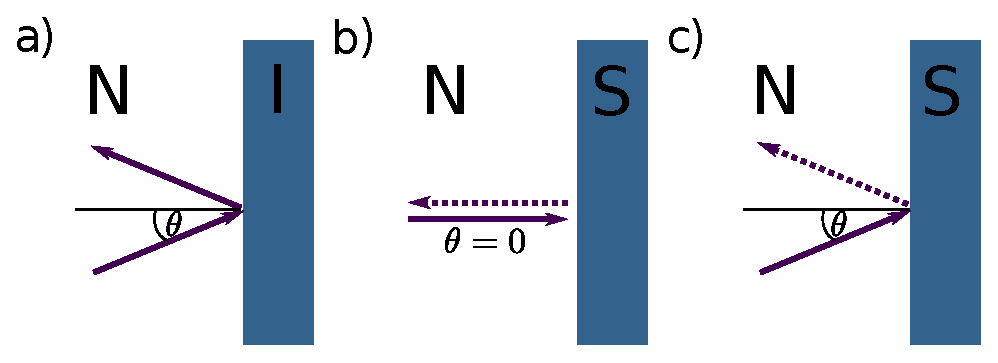
\includegraphics[width=0.7\textwidth]{figure/framework-analytical/specular-reflection}
\caption{Reflection processes. Solid arrows represent electrons, dashed arrows represent holes. \\ a) Specular reflection of an electron at an insulating interface (I). \\ b) Andreev retro reflection of an electron with into a hole. \\ c) Specular Andreev reflection of an electron into an hole with incident angle $\theta \neq 0$.}\label{fig:specular-sns}
\end{figure}

 


\chapter{A framework for the numerical model}
\label{ch:basics-numerical}
\section{Tight binding model for graphene}
%%%%%%
Tight binding models are simple, yet powerful methods to calculate the electronic band structure of a system consisting of many lattice sites. Each lattice site is represented in the Hamiltonian as an atomic potential. 
The basic premise is that the solution to the Schr\"odinger equation of the isolated system, an electron at a specific site in an atomic potential, is known. The wave function of this electron interacting with the whole lattice (interacting with all other atomic potentials from the other lattice sites) can be constructed from the overlap of the atomic wave functions. 
Following the notation in \cite{McCann2012} and also from \cite{CastroNeto2009}, the atomic orbital is denoted with $\phi_m$. This is the orbital of an atom for unit cell index $m$, where $m = 1, \dots M$. From these orbitals $\phi_m$, a Bloch state $\Phi_m$ is constructed. This Bloch state then represents the lattice symmetry (vertauscht mit dem Translationsoperator).
\begin{equation}
\Phi_m \left( \mathbf{k}, \mathbf{r} \right) = \frac{1}{\sqrt{N}} \sum_{i = 1}^N e^{i \mathbf{k} \mathbf{R}_{m, i}} \phi _m \left( \mathbf{r} - \mathbf{R}_{m, i} \right)
\end{equation}
$\Phi_m \left( \mathbf{k}, \mathbf{r} \right)$ is the Bloch state, the index $i$ labels the unit cell, with $i = 1, \dots N$ (for each unit cell there are $M$ orbitals). $\mathbf{R}_{m, i}$ is the position vector of orbital $m$ in unit cell $i$. Using this new state, the electronic wave function can be expressed as a linear combination of these orbitals
\begin{equation}
\Psi_j \left( \mathbf{k}, \mathbf{r} \right) = \sum_{m=1}^M \psi_{j, m} \left( \mathbf{k} \right) \Phi_m \left( \mathbf{k}, \mathbf{r} \right) 
\end{equation}
with coefficients $\psi_{j, m}$.
The energy of the Hamiltonian $\mathcal{H}$ is given by 
\begin{equation}
E_j \left( \mathbf{k} \right) = \frac{\langle \Psi_j| \mathcal{H} | \Psi_j \rangle}{\langle \Psi_j | \Psi_j \rangle}
\end{equation}
the coefficients can be found by minimising $E_j$. Introducing the transfer integral matrix $H$ and the overlap integral matrix $S$, one can write
\begin{equation}
H \psi_j =  E_j S_j \psi_j
\end{equation}
The coefficients of the transfer matrix and the overlap matrix are given by
\begin{eqnarray}
H_{m, m'} &=& \langle \Phi_m | \mathcal{H} | \Phi_{m'} \rangle \\
S_{m, m'} &=& \langle \Phi_m | \Phi_{m'}\rangle
\end{eqnarray}
So, in order to find the band energies $E_j$, these coefficients $H_{m, m'}$ and $S_{m, m'}$ need to be determined. Once they have been calculated, the energies can be found by solving
\begin{equation}
\text{det} \left[ H - E_j S \right] = 0
\end{equation}

\subsection{Monolayer graphene}

Let us apply the introduced procedure to monolayer graphene. Graphene has two atoms per unit cell and  one $2p_z$ orbital per atom is taken into account. Graphene has two sets of lattice vectors, $\mathbf{a_1}$, $\mathbf{a_2}$ and $\mathbf{b_1}$, $\mathbf{b_2}$, depending on which the lattice site (see figure XY). The sublattices are labelled $A$ and $B$. The atomic orbitals are therefore also labelled with a sublattice index, $\phi_A$ and $\phi_B$. The transfer matrix $H$ is
\begin{eqnarray}
H &=& \begin{pmatrix}
\phi_A^* \mathcal{H} \phi_A & \phi_A^* \mathcal{H} \phi_B \\
\phi_B^* \mathcal{H} \phi_A & \phi_B^* \mathcal{H} \phi_B\\
\end{pmatrix} \\
&\equiv& \begin{pmatrix}
H_{A A} & H_{A B} \\
H_{B A} & H_{B B}\\
\end{pmatrix}
\end{eqnarray}
For the diagonal elements, $H_{A A}$ and $H_{B B}$, the strongest contribution comes from the interaction of the orbital with itself. The hopping from one $A$ site to another $A$ site is significantly smaller and is therefore neglected. (Makes sense, since the nearest neighbours of an $A$ site are $B$ sites).
\begin{equation}
H_{A A} \approx \frac{1}{N} \sum_{i=1}^N \langle \phi_A ( \mathbf{r} - \mathbf{R}_{A, i} ) | \mathcal{H} |  \phi_A ( \mathbf{r} - \mathbf{R}_{A, i} ) \rangle \equiv \epsilon_A
\end{equation}
$H_{B B} = \epsilon_B$ holds in the analogous way. Since graphene has two identical sublattices $A$ and $B$, the on-diagonal energies are equal: $\epsilon_A = \epsilon_B$. 
Off diagonal elements $H_{A B}$ and $H_{B A}$ describe the possibility of hopping from one sublattice to the other. 
\begin{eqnarray}
H_{A B } &\approx & \frac{1}{N} \sum_{i = 1}^N \sum_{l = 1}^3 e^{i \mathbf{k} \bm{\delta}_l} \langle \Phi_A ( \mathbf{r} - \mathbf{R}_{A, i} ) | \mathcal{H} | \Phi_B ( \mathbf{r} - \mathbf{R}_{A, i} - \bm{\delta}_l ) \rangle  \\
& \equiv & - \gamma_0 f \left( \mathbf{k} \right) \label{eq:gamma0},
\end{eqnarray}
where
\begin{eqnarray}
\gamma_0 &=& - \langle \Phi_A ( \mathbf{r} - \mathbf{R}_{A, i} )| \mathcal{H} | \Phi_B ( \mathbf{r} - \mathbf{R}_{A, i} - \bm{\delta}_l ) \rangle \\
f \left( \mathbf{k} \right) &=&  \sum_{l = 1}^3 e^{i \mathbf{k} \bm{\delta}_l} 
\end{eqnarray}
$\bm{\delta}_l$ gives the distance vectors from one given $A$ atom to another $B$ site. The other off-diagnoal element of $H$ is $H_{B A} = H_{A B}^* = - \gamma_0 f^* \left( \mathbf{k} \right)$. The overlap matrix elements on the diagonal, $S_{A A}$ and $S_{B B}$ equal to one, since 
\begin{equation}
S_{A A} = S_{B B} = \langle \Phi_A ( \mathbf{r} - \mathbf{R}_{j, i} ) | \Phi_A ( \mathbf{r} - \mathbf{R}_{j, i} ) \rangle = 1.
\end{equation}
For the off-diagonal elements, similar to eq. (\ref{eq:gamma0}), a coefficient $s_0$ is introduced.
\begin{eqnarray}
S_{A B} &=& S_{B A} = s_0 f \left( \mathbf{k} \right) \\
s_0 &=& \langle \Phi_A ( \mathbf{r} - \mathbf{R}_{A, i} ) | \Phi_B ( \mathbf{r} - \mathbf{R}_{B, l} ) \rangle 
\end{eqnarray}
Finalizing, the Hamiltonian $H$ and the overlap integral matrix $S$ are
\begin{eqnarray}
H &=& \begin{pmatrix} \epsilon_1 & - \gamma_0 f \left( \mathbf{k} \right) \\ - \gamma_0 f^* \left( \mathbf{k} \right) & \epsilon_B \end{pmatrix} \\
S &=& \begin{pmatrix} 1 & s_0 f \left( \mathbf{k} \right) \\ s_0 f^* \left( \mathbf{k} \right) & 1 \end{pmatrix}
\end{eqnarray}
The energy $\gamma_0$ and the coefficient $s_0$ have been determined experimentally \cite{Dresselhaus1995}:
$\gamma_0 = 3.033 \text{eV}$ and $s_0 = 0.129$.

\subsection{Bilayer graphene}
Bilayer graphene consists of two layers of graphene, and each of these layers has two sublattices. A lattice site in bilayer graphene can there be in one of the four sublattices $A_1$, $B_1$, $A_2$ and $B_2$, where the integer 1, 2 labels the layer. Using the notation of the SWM model, \cite{McClure1957}, \cite{McClure1960}, the transfer matrix can be written as
\begin{equation}
H =  \begin{pmatrix} \epsilon_{A_1} & - \gamma_0 f \left( \mathbf{k} \right) & \gamma_4 f \left( \mathbf{k} \right) & - \gamma_3 f^*\left( \mathbf{k} \right) \\
- \gamma_0 f^* \left( \mathbf{k} \right) & \epsilon_{B_1} & \gamma_1 & \gamma_4 f \left( \mathbf{k} \right) \\
\gamma_4 f^* \left( \mathbf{k} \right) & \gamma_1 & \epsilon_{A_2} & - \gamma_0 f \left( \mathbf{k} \right)  \\
- \gamma_3 f \left( \mathbf{k} \right) & \gamma_4 f^* \left( \mathbf{k} \right)& -\gamma_0 f* \left( \mathbf{k} \right)& \epsilon_{B_2} \end{pmatrix} \label{eq:bilayer-matrix}
\end{equation}
The basis  of this matrix is  $( |\phi_{A_1}\rangle$, $|\phi_{B_1}\rangle$, $|\phi_{A_2}\rangle$, $|\phi_{B_2}\rangle )$ and therefore describes an $AB$-stacked bilayer system. If the representation of eq (\ref{eq:bilayer-matrix}) had the basis $( |\phi_{B_1}\rangle$, $|\phi_{A_1}\rangle$, $|\phi_{A_2}\rangle$, $|\phi_{B_2}\rangle )$, the matrix would describe an $AA$-stacked bilayer system. %TODO see figure...
In an $AB$ ($AA$) stacked system, an $A_2$ atom would be directly above an atom of the $B_1$ ($A_1$) sublattice.

In the most general case, the energies $\epsilon$ on the diagonal are not equal. The off-diagonal parameters $\gamma$ are given by
\begin{eqnarray}
\gamma_0 &=& - \langle \phi_{A_1} | \mathcal{H} | \phi_{B_1} \rangle = - \langle \phi_{A_2} | \mathcal{H} | \phi_{B_2} \rangle, \\
\gamma_1 &=& ~\langle \phi_{A_2} | \mathcal{H} | \phi_{B_1} \rangle, \\
\gamma_3 &=& - \langle \phi_{A_1} | \mathcal{H} | \phi_{B_2} \rangle, \\
\gamma_4 &=& ~\langle \phi_{A_1} | \mathcal{H} | \phi_{A_2} \rangle = \langle \phi_{B_1} | \mathcal{H} | \phi_{B_2} \rangle
\end{eqnarray}
The $\gamma_0$ parameter describes nearest neighbour hopping within a layer (in-plane hopping) and does therefore contain the factor $f\left( \mathbf{k} \right)$, which is defined as the distance to the surrounding neighbours in one layer. %TODO include definition?
Interlayer hopping between $A_2$ and $B_1$ atoms is included with the parameter $\gamma_1$. This hopping is vertical from one layer to the other. The parameters $\gamma_3$ and $\gamma_4$ also describe interlayer hopping, but this hopping is not vertical (it does not connect lattice sites that are directly in line). It can be though of as a combination of in-plane hopping followed by vertical hopping (see figure).
%TODO figure with hoppings
The overlap matrix of bilayer graphene can be introduced with the parameters $s_0 = \langle \Phi_{A_1} | \Phi_{B_1} \rangle = \langle \Phi_{A_2} | \Phi_{B_2} \rangle $ and $s_1 = \langle \Phi_{A_2}  | \Phi_{B_1} \rangle $ \cite{Mucha-Kruczynski2010}. The parameters $s_3$ and $s_4$ are neglected, because they are small (why?).
\begin{equation}
S = \begin{pmatrix}
1 & s_0 f\left( \mathbf{k} \right)& 0 & 0 \\
s_0 f^*\left( \mathbf{k} \right) & 1 & s_1 & 0 \\
0 & s_1 & 1 & s_0 f\left( \mathbf{k} \right) \\
0 & 0 & s_0 f^* \left( \mathbf{k} \right) & 1\\
\end{pmatrix}
\end{equation}
The overlap matrix $S$ is often approximated as a unit matrix and the parameters $s_0$ and $s_1$ are neglected. These parameters $s_0$ and $s_1$ describe the non-orthogonality of orbitals, which is small for energies $E \leq \gamma_1$.

The tight binding parameters can be determined experimentally using Raman scattering \cite{Malard2007} or infrared spectroscopy \cite{Kuzmenko2009}. The values determined in \cite{Kuzmenko2009} are
\begin{eqnarray}
\gamma_0 &=& 3.16,
\gamma_1 = 0.381, 
\gamma_3 = 0.38,
\gamma_4 = 0.14.
\end{eqnarray}

\subsection{Model used in kwant}

The bilayer system that is used in this thesis is $AB$-stacked. The Hamiltonian that is used in the \texttt{kwant} software is
\begin{equation}
H = - t \sum_{i, j} e^{i \phi_{i, j }} a^\dagger_{m, i} b_{m, i} - \gamma_1 \sum_j a_{1, j}^\dagger b_{2, j} - \sum_{i, m} \left( \mu_i - (-1)^m \delta_i\right) \left(a^\dagger_{m, i} a_{m, i} + b^\dagger_{m, i} b_{m, i} \right).
\end{equation}
\begin{equation}
H = - \gamma_0 \sum_{i, j} e^{i \phi_{i, j }} a^\dagger_{m, i} b_{m, i} - \gamma_3 \sum_j a_{1, j}^\dagger b_{2, j} - \sum_{i, m} \left( \mu_i - (-1)^m \delta_i\right) \left(a^\dagger_{m, i} a_{m, i} + b^\dagger_{m, i} b_{m, i} \right).
\end{equation}

For implementing the system in kwant, the tight binding model hast to be defined. Means, lattice with corresponding symmetry has to be build and the hoppings between the lattice points have to be definded.
First adaption: magnetic field has to be included. It enters in form of a phase (Peierls substitution):
\begin{equation}
\phi_{i, j} = \frac{e}{\hbar} \int_i^j \mathbf{A} d\mathbf{r}
\end{equation}
The parameters X and Y are neglected, the Hamiltonian is of the form

$m = 1, 2$ is index of the layer. The operators $a^\dagger_{m, i},\ a_{m, i}$ create and annihilate an electron of sublattice $A$ on layer $m$ at site $i$. In the same way, $b^\dagger_{m, i},\ b_{m, i}$ are the creation and annihilation operators for the sublattice $B$. The intralayer hopping parameter $t$ is the same as $\gamma_0$ from above and $\gamma_1$ is the known interlayer (between dimer) hopping parameter. 
%TODO not sure of the interlayer hopping parameter is really gamma1 from mccann or SWM model? matrix element / hopping corresponds to gamma_3....
The onsite energies are
\begin{eqnarray}
\epsilon_{A_1} = \epsilon_{B_1} = \mu_i + \delta_i \\
\epsilon_{A_2} = \epsilon_{B_2} = \mu_i - \delta_i \\
\end{eqnarray}
Here, $\mu$ and $\delta$ are defined as 
\begin{eqnarray}
\mu_i &=& \frac{\varphi_{BG} + u_i \varphi_{SG}}{2} \\
\delta_i &=& \frac{\varphi_{BG} -  u_i \varphi_{SG}}{\eta}
\end{eqnarray}
$u_i$ is used as a paramter that defines, if the lattice site $i$ is within a gated region ($u_i = 1$) (underneath a topgate) or not ($u_i = 0$).

\section{Random matrix theory for transport}

\subsection{Basics about the random matrix theory}

To describe the transport through a conducting region of interest, which is in between of two ideal leads. Ideal leads means that there is no disorder present, whereas the conductor is a disordered system. The question that the random matrix theory is answering, is: how can one describe the transport from one lead, through the disordered region to the other lead? Essential for this transport theory is the work of Landauer (cite!), who described ballistic transport through a 1D channel as a transmission problem. 

The transport through the conducting region can be written in terms of an incident wave $c^\text{in}$ and a reflected/transmitted wave $c^\text{out}$. The scattering matrix $\mathcal{S}$ relates the amplitudes of these wave functions.
\begin{equation}
c^{\text{out}} = \mathcal{S} c^{\text{in}},
\end{equation}
where
\begin{eqnarray}
c^\text{in} &=& \left( a_1^+, a_2^+, \dots a_N^+, b_1^+, b_2^+, \dots b_N^+ \right) \\
c^\text{out} &=& \left( a_1^-, a_2^-, \dots a_N^-, b_1^-, b_2^-, \dots b_N^- \right)
\end{eqnarray}
The coefficients $a$ represent the left lead and $b$ the right lead. The $\pm$ sign indicates, if it describes a right or left moving electron (see figure). The integer $n = 1, 2, \dots N$ is the index for the propagating modes. In this case, there are $N$ modes in both the left and the right lead. %TODO ?
%TODO figure
The scattering matrix has the form
\begin{equation}
\mathcal{S} = \begin{pmatrix} r & t' \\ t & r'\end{pmatrix}
\end{equation}
where $r,\ r'$ are reflection matrices, and $t,\ t'$ are $N \times N $ transmission matrices. Both the transmission and the reflection matrices have the dimension $N \times N$. The scattering matrix is unitarity, since the current is conserved:
\begin{equation}
\mathcal{S}^{-1} = \mathcal{S}^\dagger.
\end{equation}
Consequently, the matrices $tt^\dagger$, $t't^\dagger$, $1-rr^\dagger$ and $1-r'r^\dagger$ have the same set of eigenvalues $T_1, T_2, \dots T_N$, each of them being a real number between $0$ and $1$.

It is useful to write the scattering matrix $\mathcal{S}$ in terms of the transmission eigenvalues $T_n$, introducing the matrix $\mathcal{T} = \text{diag} ( T_1, T_2, \dots T_n )$. Each of the eigenvalues of $\mathcal{T}$ is a real value between 0 and 1. This rewriting is done in \cite{Mello1988} and is called polar decomposition
\begin{equation}
\mathcal{S} = \begin{pmatrix} U & 0 \\ 0 & V\end{pmatrix} \begin{pmatrix} - \sqrt{1 - \mathcal{T}} & \sqrt{\mathcal{T}} \\ \sqrt{\mathcal{T}}& \sqrt{1 - \mathcal{T}} \end{pmatrix} \begin{pmatrix} U' & 0 \\ 0 & V' \end{pmatrix}
\end{equation}
$U$, $V$ are are $N\times N $ unitary matrices, I dont know why they are useful.

%TODO rewrite below, 
The scattering matrix relates incoming ($c^\text{in}$) states to outgoing ($c^\text{out}$) states. It is also possible to look at the transfer matrix $M$, which relates states from the left lead ($c^\text{left}$) to states in the right lead ($c^\text{right}$):
%TODO figure
\begin{equation}
c^\text{right} = M c^\text{left}
\end{equation}
where 
\begin{eqnarray}
c^\text{left} &=& \left( a_1^+, a_2^+, \dots, a_N^+, a_2^-, a_2^-, \dots a_N^-\right) \\
c^\text{right} &=& \left( b_1^+, b_2^+, \dots, b_N^+, b_2^-, b_2^-, \dots b_N^-\right) \\
M &=& \begin{pmatrix} V & 0 \\ 0 & V'^\dagger \end{pmatrix} \begin{pmatrix} \sqrt{\mathcal{T}^{-1}} & \sqrt{\mathcal{T}^{-1} -1} \\ \sqrt{\mathcal{T}^{-1} -1} & \sqrt{\mathcal{T}^{-1}}\end{pmatrix} \begin{pmatrix} U' & 0 \\ 0 & U\dagger \end{pmatrix}
\end{eqnarray}

Both the transfer matrix $M$ and the scattering matrix $S$ describe the conductive region. The nice feature of the transfer matrix can be seen, if multiple disordered regions, each separated by ideal leads, are considered. The transfer matrix of the whole system is a multiplication of each regions individual transfer matrix. (which is an advantage, the scattering matrix stuff is then a bit of a fuck off...)
%TODO das fällt son bisschen ausm Himmel...
The conductance of such a disordered region is given by the sum of the transmission eigenvalues $T_n$:
\begin{equation}
G = G_0 \sum_{n=1}^N T_n, \quad G_0 = \frac{2e^2}{h}
\end{equation}
This is cool. But there is not much context...

\subsection{Supercurrent of a SNS junction in the scattering matrix approach}

Considering an SNS junction. The wave funtions for an incident wave and an reflected/transmitted wave contain now coefficients for electrons and holes:
\begin{eqnarray}
c_N^\text{in} &=& \left( c^+_e(N_1), c^-_e(N_2), c^-_h(N_1), c^+_h(N_2) \right) \\
c_N^\text{out} &=& \left( c^-_e(N_1), c^+_e(N_2), c^-_h(N_1), c^+_h(N_2) \right)
\end{eqnarray}
$N_1$ is the number of modes in the left lead, $N_2$ is the number of modes in the right lead. In the special case of scattering between a normal conductive region and a superconductor, two types of scattering have to be distinguished. For one, there is the normal scattering of electrons and there is Andreev reflection of electrons at the superconductor. The scattering process at the normal region is described by the normal scattering matrix $s_N$, that connects an incident wave with a reflected/transmitted one.
\begin{equation}
c^\text{out}_N = s_N(\epsilon) c^\text{in}_N
\end{equation}
This scattering matrix $s_N$ is
\begin{equation}
s_N (\epsilon) = \begin{pmatrix} s_0 (\epsilon ) & 0  \\ 0 & s_0 ( \epsilon) \end{pmatrix} \label{eq:s-n},
\end{equation}
where
\begin{equation}
s_0 = \begin{pmatrix} r_{1 1} & t_{1 2} \\ t_{2 1} & r_{2 2} \end{pmatrix}
\end{equation}
The Andreev reflection process is described by another scattering matrix, the Andreev scattering matrix $s_A$. For  energies $\epsilon < \Delta$, there are no propagating modes inside the superconductor.  And for $\Delta_0 \ll E_F$, the normal reflection at the NS interface can be ignored and only Andreev scattering is taken into account.
\begin{equation}
s_A = \alpha(\epsilon) \begin{pmatrix} 0 & r_A \\ r_A^* & 0 \end{pmatrix}, 
\end{equation}
with $\alpha ( \epsilon ) = \text{exp} \left( -i \arccos \frac{\epsilon}{\Delta} \right) $
\begin{equation}
r_A = \begin{pmatrix} e^{i \phi /2 } \mathds{1} & 0 \\ 0 & e^{-i \phi / 2 } \mathds{1} \end{pmatrix}
\end{equation}
From the structure of the Andreev scattering matrix, it can be seen that an electron mode is transformed into a hole mode, while the mode index $n$ does not change. This transformation is accompanied by a phase shit of $- \arccos \frac{\epsilon}{\Delta} $, which comes form the decay into the superconducting region. Also, a phase of $\phi/2$ ($-\phi/2$), where $\phi$ is the superconducting phase difference, is added for reflection from electron to hole (hole to electron).


A bound state in the SNS junction forms, when 
\begin{equation}
c_\text{in} = s_A ( \epsilon ) s_N ( \epsilon ) c_\text{in} \label{eq:bound-state-cond}
\end{equation}
holds. In the short junction limit, $L \ll \xi$, it holds that
\begin{equation}
s_0 ( \epsilon ) \approx s_0 ( - \epsilon ) \approx s_0 ( 0) \equiv s_0
\end{equation}
This can be used to simplify the normal scattering matrix $s_N (\epsilon) $ equation (\ref{eq:s-n}). Using this approximation, the bond state condition eq. (\ref{eq:bound-state-cond}) becomes
\begin{equation}
\begin{pmatrix} s_0^\dagger & 0\\ 0 & s_0^T \end{pmatrix}  \begin{pmatrix} 0 & r_A^* \\ r_A & 0 \end{pmatrix}  c_\text{in} = \text{exp} \left( i \arccos \frac{\epsilon}{\Delta} \right) c_\text{in}
\end{equation}
This can be simplified further. By appliying a Joukowsky (magic) transformation, that i do not understand yet, it is possible to write
\begin{equation}
\begin{pmatrix} 0 & - i A \\ i A & 0 \end{pmatrix} c_\text{in} = \frac{\epsilon}{\Delta}
\end{equation}
with $A = \frac{1}{2} ( r_A s_0 - s_0^T r_A)$ . This leads  to
\begin{equation}
A^\dagger A c_\text{in} = \frac{\epsilon^2}{\Delta^2} c_\text{in} \label{eq:bound-state-final}
\end{equation}

So far, the condition for an Andreev bound state has been simplified according to the short junction approach. To get an expression for the current, the free energy $F$ is needed \cite{Beenakker1992}:
\begin{equation}
I = \frac{ 2 e}{\hbar} \frac{d F}{d \phi}
\end{equation}
the free energy $F$ has been calculated as \cite{Beenakker1991}
\begin{equation}
F = - 2 k_B T \sum_{\epsilon > 0 } \text{ln} \left[ 2 \cosh \frac{\epsilon}{2 k_B T}  \right] + \dots
\end{equation}
which is the free energy of a non interacting electron . 
So the current is
\begin{equation}
I = - \frac{2 e}{\hbar} \sum_p \tanh \left( \frac{\epsilon_p}{2 k_B T} \right) \frac{d \epsilon_p }{d \phi}
\end{equation}
The derivation of the energy with respect to the phase can be obtained from eq. (\ref{eq:bound-state-final}).
\begin{equation}
\frac{d \epsilon}{d \phi } = \frac{\Delta^2}{2 \epsilon} \frac{\langle c_\text{in} | \frac{d ( A^\dagger A )}{d \phi }| c_\text{in} \rangle} {\langle c_\text{in} |c_\text{in} \rangle}
\end{equation}

%\subsection{Implementation in kwant} ?

\chapter{Experimental set-up}
\label{ch:experiment}

\section{First: summary of paper}
\subsection{Introduction}

\begin{figure}
\centering
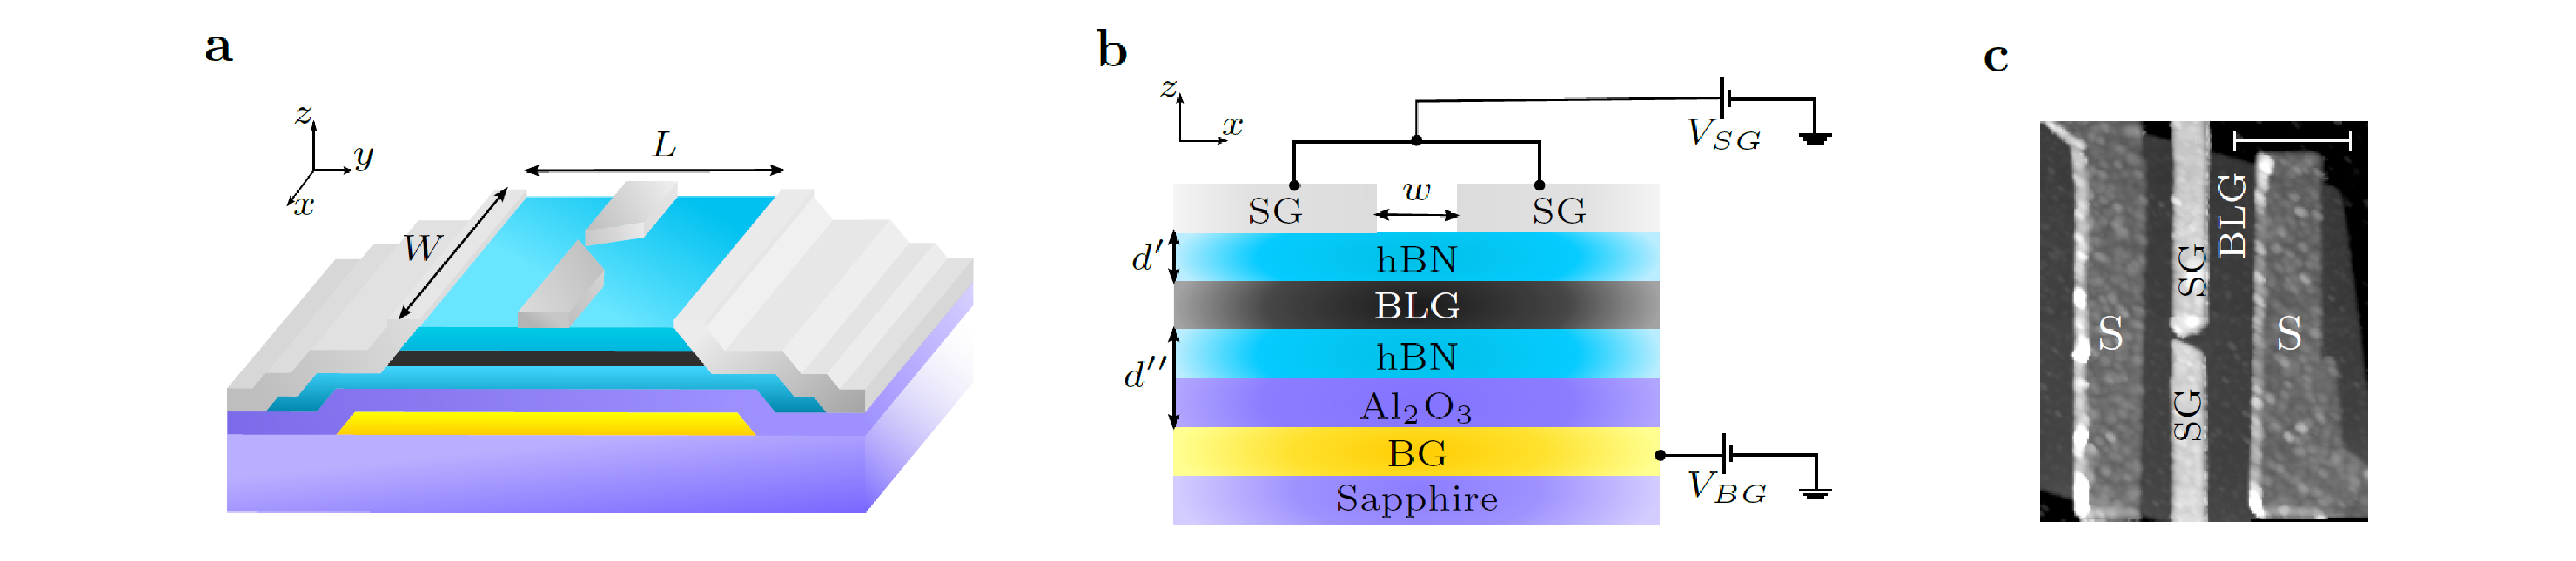
\includegraphics[width=0.8\textwidth]{figure/experiment/setup}
\end{figure}

Josephson effect \cite{Josephson1962} has been studied a lot. Key challenge: Developing devices in which the induced superconductivity can be monitored. This experiment is cool, because it uses local gates to control confinement, amplitude and density profile of the supercurrent. The sample used is a BLG-HBN-VDW heterostructure.
Tunnel barrier -> supercurrent can only be tuned by modifying the geometry/temperature.
Weak link -> a conductive material, in which superconductivity can be induced (proximity effect) and supercurrent can flow over larger distance than in tunnel junction \cite{Likharev1979}.
Magnitude of supercurrent depends on contact transparency, disorder in the weak link, temperature.

Greatness of this work: full control of supercurrent both in amplitude and spatial distribution has not been observed so far. It is difficult to confine charge carriers in graphene (SLG!), because no backscattering in graphene and Klein tunneling \cite{Katsnelson2006}. Using BLG helps, because one can engineer an electronic band gap forming the barrier. 

Sample geometry: QPC-like split gate geometry. The sample is overall gated with a backgate $V_{BG}$, a local top-gate in shape of two fingers (QPC geometry) is used to build a barrier. How does this process work? The overall backgate pushes the fermi level up into the conductance band. The topgate gives a displacement field, it pushes the fermi level down into the band gap --> no conduction possible, insulating state induced.
Asymmetry between the layers of bilyer graphene (different energies at the layer) opens a band gap \cite{McCann2006} that is tuneable.

\subsection*{Normal state analysis:}
\begin{itemize}
\item low charge carrier density $2.8\cdot 10^{18}$.
\item Landau fans in magnetotransport measurement
\item Fabry Perot interferences
\end{itemize}

\subsubsection*{On the resistance maps}
\begin{figure}
\centering
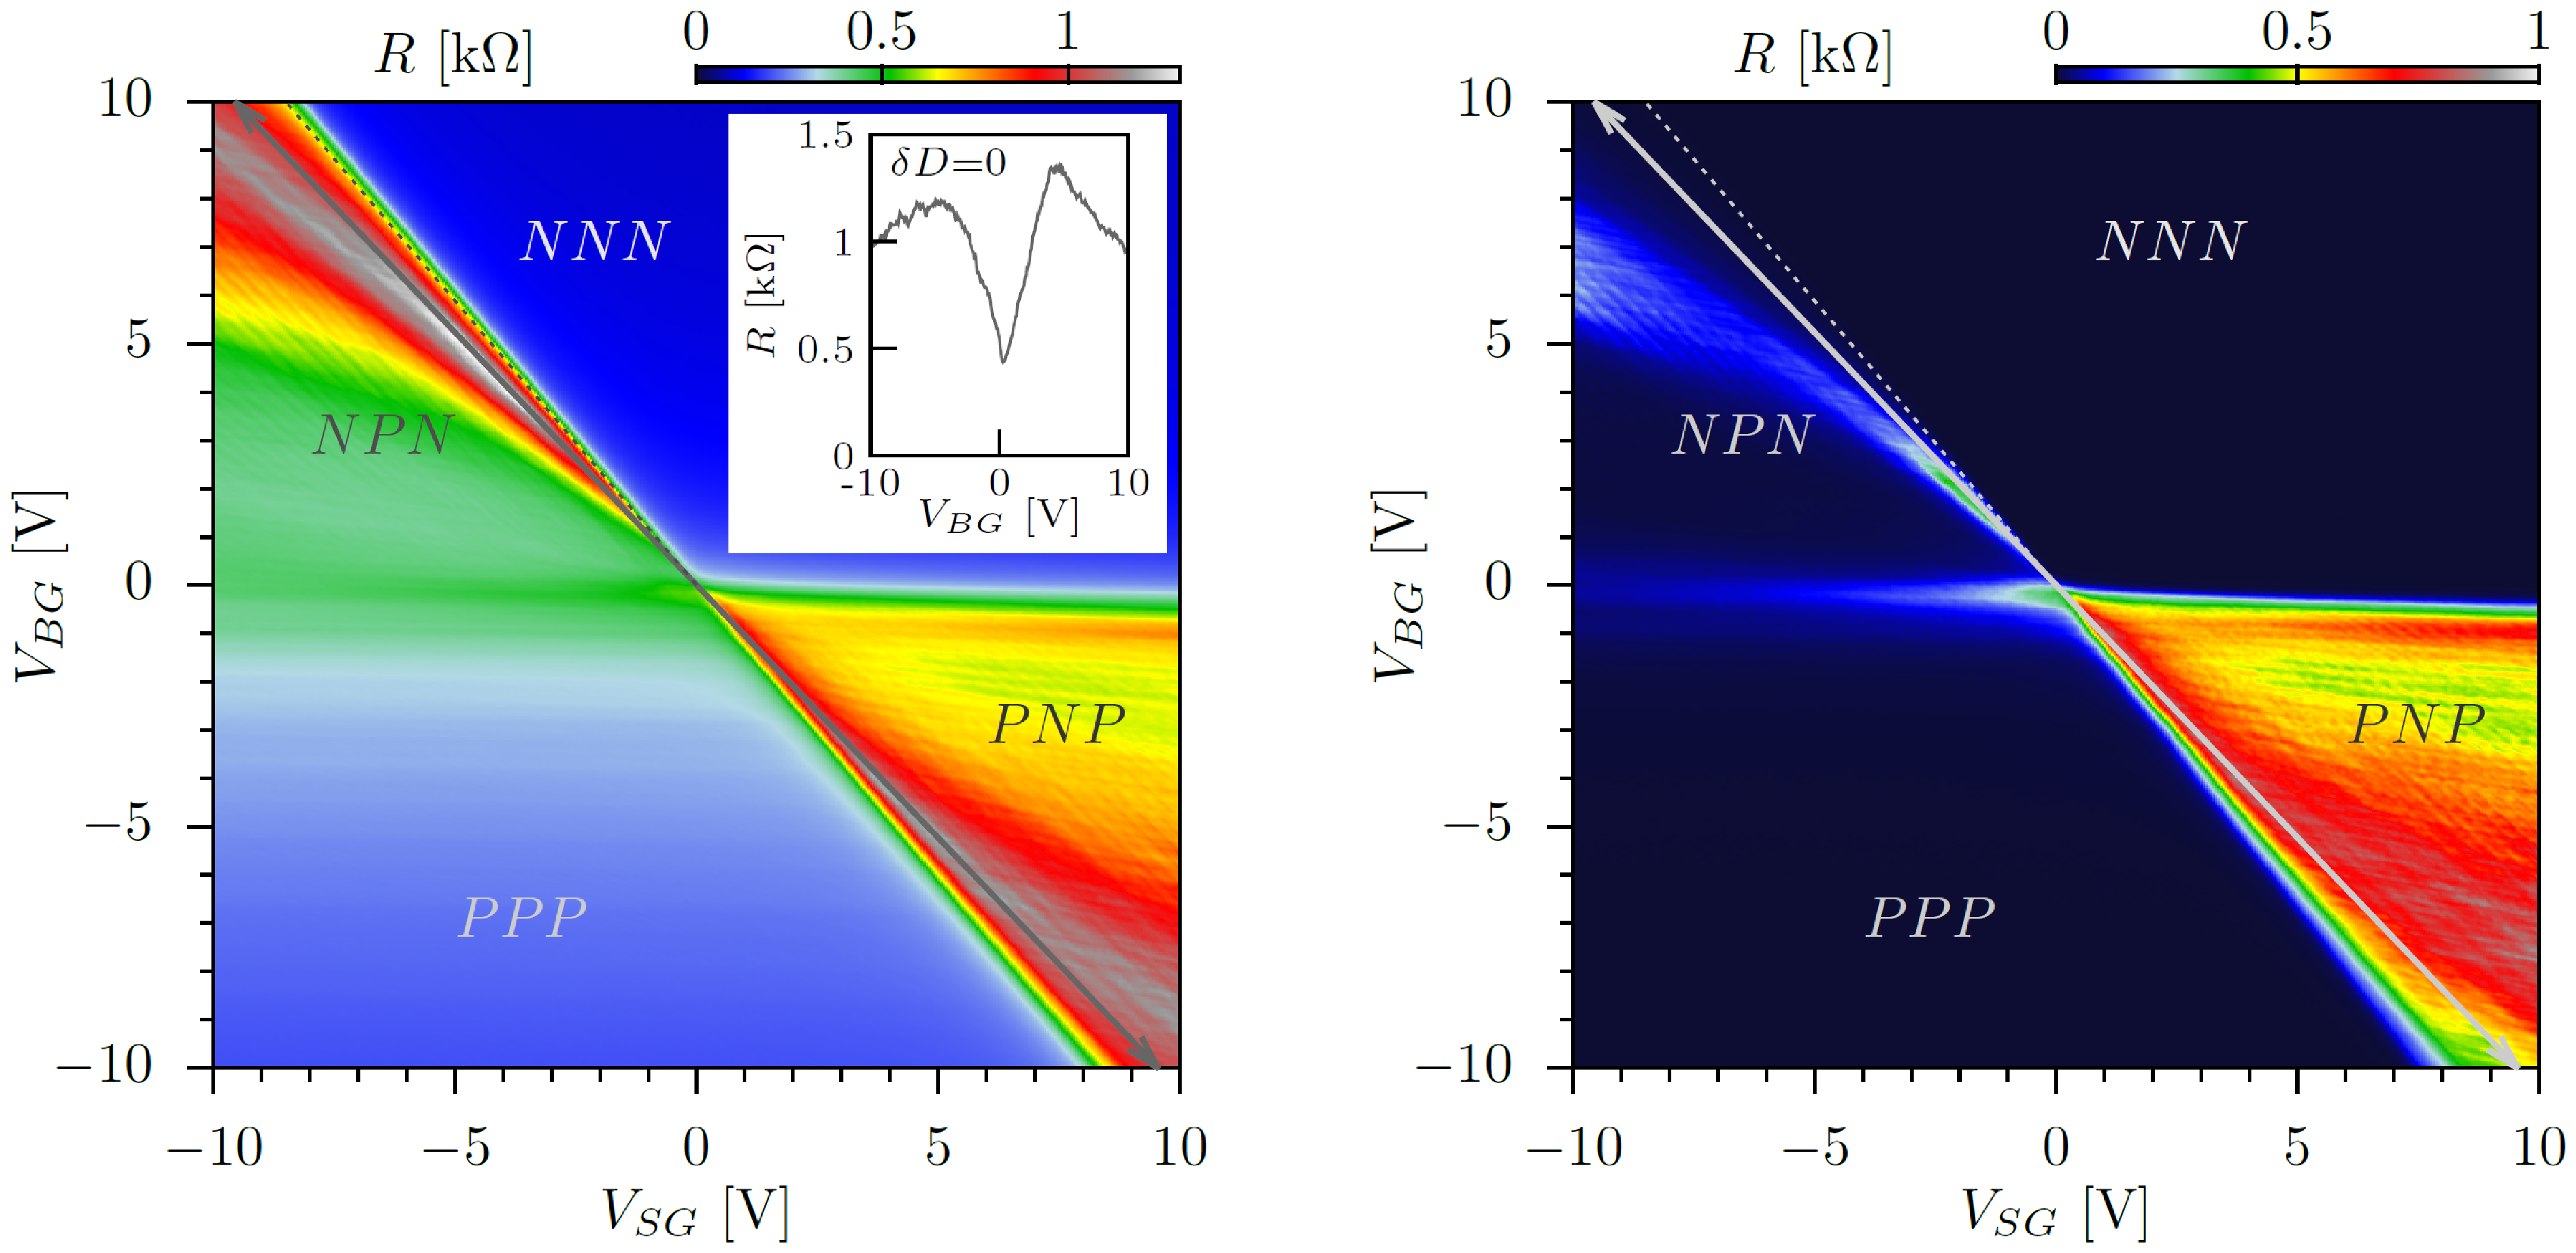
\includegraphics[width=0.8\textwidth]{figure/experiment/resistance-map-edit}
\caption{Resistance maps}
\end{figure}

 The gate map has the backgate as y-axis, the splitgate (QPC topgate) as x-axis and the color indicates the strength of measured resistane. For orientiation, the line where back and splitgate are equal is called the displacement field line (grey arrow). Naming the regions, depending on the position of the fermi level: fermi level in valence band: N, fermi level in conductance band: P. Think of it as three regions: BLG backgated, the area where BLG is back and topgated (region with topgates on top of the material), and again a region where BLG is only backgated. Depending on the the choice of $V_{BG}$ and $V_{SG}$, there are four regions: NNN, NPN, PPP, PNP. Looking at the upper left quadrant, NPN. In this region, the maximum resistance seems to follow the displacement field line (grey arrow), until a certain point, where it bends and the maximum resistance is not on a straight line anymore. Effect is visible in the normal state but even more in the superconducting state. --> unexpected behaviour.
 
Explanation? Charge carrier density is low, the influence of the backgate is important. The higher the backgate value is, the less the charge carrier density is affected by the splitgate and the stray fields, that it produces. And, as the splitgate impact is weak, the device stays conductive (resistance is low) along the displacement field line. 
Why the bending? In the upper region of the displacement field line, the split gates work as intenden: the channel region (the region, where the supercurrent can pass through) is conductive, because the backgate dominates. In the region, where the resistance curve is bending, the stray fields from the splitgate dominate, effectively blocking the channel region and therefore leading to to increased resistance.

The overall resistance is higher on the p-side, due to the slight n-doping of the leads (they create a pn junction at each contact). Can be seen in the supercondcuting state, the pnp region remains resistive, the npn region shows zero resistance.

\subsubsection*{Fabry Perot resonances}

gate dependece of conductance shows oscillatory behaviour, are attributed to Fabry Perot interferences of differenct cavities \cite{Shytov2008}


\subsection*{Superconducting state}
\begin{figure}
\centering
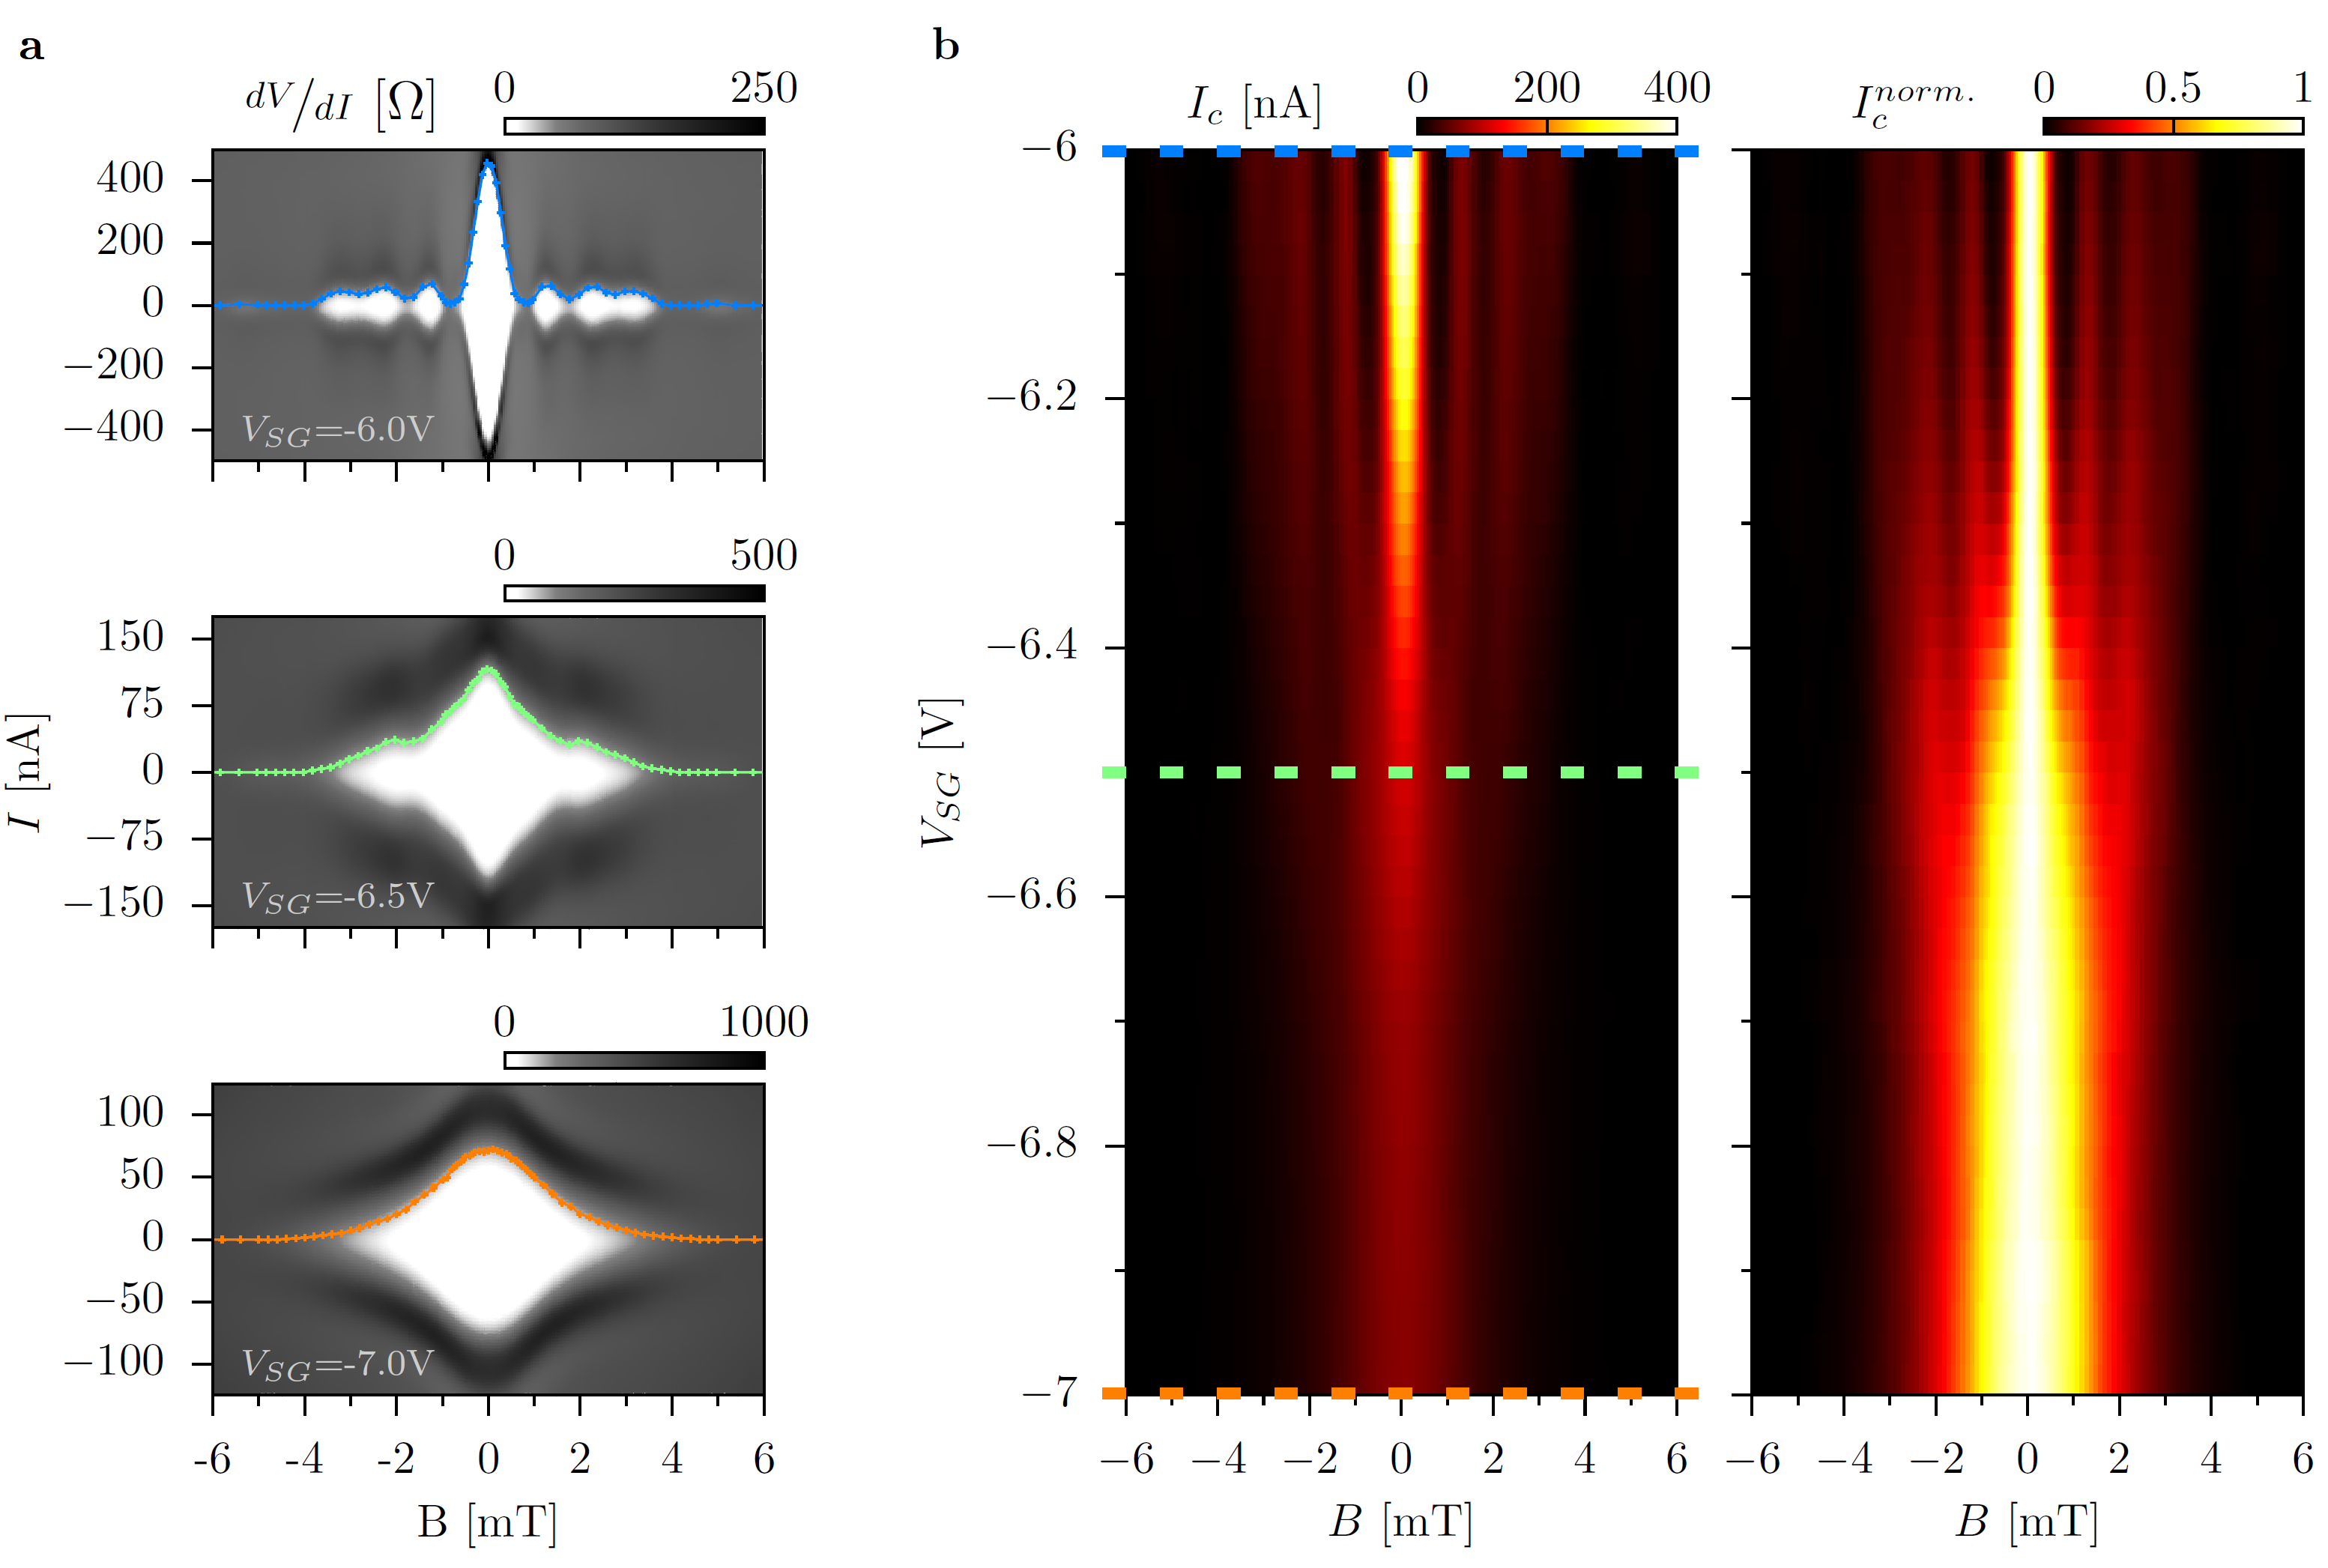
\includegraphics[width=0.8\textwidth]{figure/experiment/supercurrent}
\end{figure}

Since the device becomes superconducting in the npn region, the experiments focus on this part when analysing the supercurrent.

The amplitude of the supercurrent can be monitored by tuning the charge carrier densitiy with the backgate. 

Supercurrent density can be explored by probing the interference pattern in response to a perpendicular magnetic field.  A change of the junction geometry directly manifests within the interference pattern. 

Confinement of the current can be observerd: 
\begin{itemize}
\item open regime: Fraunhofer-like pattern, two dimensional system
\item splitgate increases: lobes are lifted
\item constriction is formed, really a 1D channel has formed: non beating, bell-shaped pattern
\end{itemize}

Transition from Fraunhofer to bell-shaped pattern has been observed before: \cite{Chiodi2012}


\chapter{Analytical Model}
\label{ch:analyticalmodel}
%\textit{This chapter presents a calculation of the critical current in a SNS junctions. For this purpose, a quasiclassical transport theory is used and its foundations are explained in the first section. This technique is then employed for a clean SNS junction, and an expression for the Josephson current is found. In the following section, the calculations used for the clean setup are extended for the more sophisticated quantum point contact (QPC) and here as well, the current for the QPC-gated junction is found.}

\section{Foundation of the quasiclassical model}
%This section explains preliminary assumptions made to describe the current in a SNS junction. 
From section \ref{sec:theory-sns} it is known that Andreev reflection of electrons in a SNS junction leads to Andreev bound states within the junction. Each one of these bound states contributes to the total current through the junction. Essentially, a bound state can be expressed as a trajectory from one superconductor through the normal metal to the other superconductor. The superconducting current density is found through geometrical analysis of possible trajectories. The total current density is then found by adding up all these trajectories.
%The superconducting current density is found by summing up these trajectories. This is a way to express the current through geometrical analysis of possible trajectories only. The underlying material does not play a specific role in the calculation, which makes this approach universally applicable.
\begin{figure}[h]
\centering	
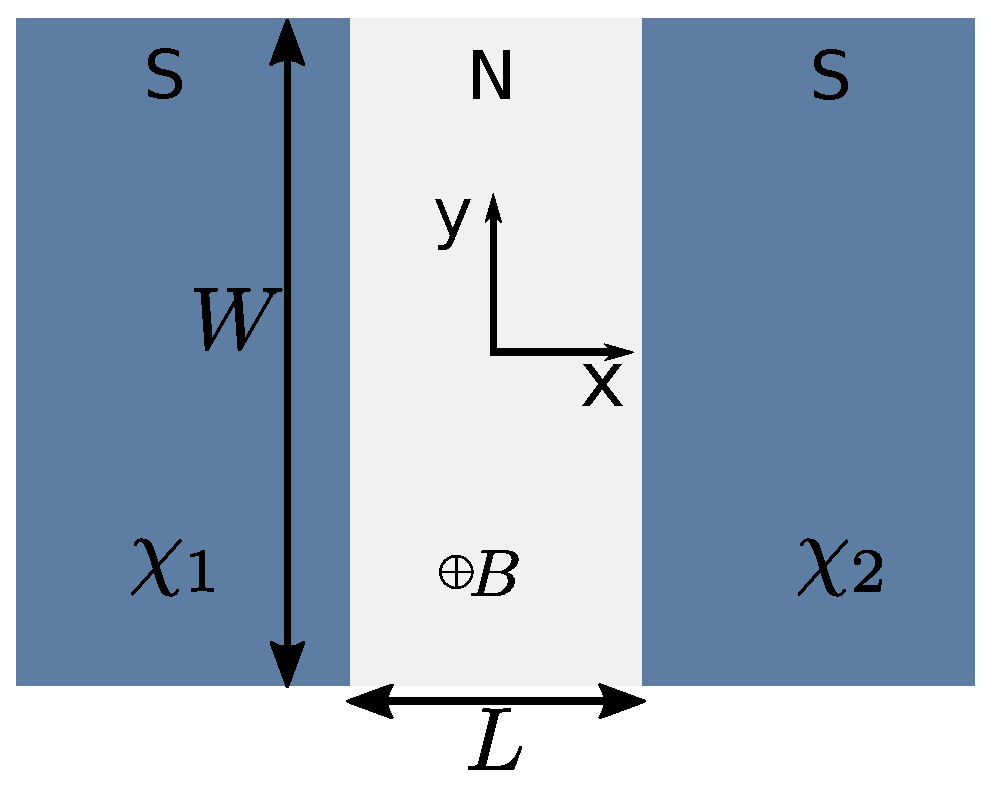
\includegraphics[width=0.5\textwidth]{figure/analyticalmodel/sns_junction}
\caption{SNS junction with width $W$ and length $L$. A trajectory connecting the interfaces is parametrized by the angle $\theta$ between the trajectory and the x-axis. $\chi_1$ and $\chi_2$ are the superconducting phases, with total phase differece $\chi = \chi_2 - \chi_1$.}
\label{fig:sns_schematic}
\end{figure}
The two dimensional junction (schematic shown in fig \ref{fig:sns_schematic}) is a short and wide junction with width $W$ and length $L$, where $W \gg L$. The NS-interfaces are parallel to the $y$-axis and are placed at $x = \pm L/2$. Each of the superconducting leads has a phase $\chi_{1}$ and $\chi_{2}$, and the overall phase difference is $\chi = \chi_{1} - \chi_{2}$. The superconducting gap parameter $\Delta$ is only present in the superconducting leads. Close to the interface, $\Delta$ begins to decay on a length scale of the superconducting coherence length $\xi_0$ into the normal region.
%\begin{equation}
%\xi_0 = \hbar v_F / \pi \Delta.
%\end{equation} 
Similar to the procedure in section \ref{sec:theory-sns}, this decay is neglected and a step-like behaviour is assumed for the superconducting gap parameter:
\begin{equation}
\Delta\left( x \right) = |\Delta| e^{\chi_1} \Theta\left(-L/2 -x \right) + |\Delta| e^{\chi_2} \Theta\left(x-L/2 \right).
\label{eq:gap_parameter}
\end{equation}
The thermal length scale of the system assumed to be larger than the sample length:
\begin{equation}
L_T = \hbar v_F / k_B T \gg L.
\end{equation}
The transport through the junction is assumed to be ballistic, resulting in the trajectories being straight and not being altered by scattering in the normal region. However, the presence of the magnetic field in the normal region of the sample will lead to a bending of the trajectories due to the Lorentz force. Depending on the strength of magnetic field $B$ and the Fermi velocity, the radius of this curve is 
\begin{equation}
r_B = \frac{m v_F}{e B}
\end{equation}
In order to justify the assumption of straight trajectories, either the magnetic field has to be weak enough, or the Fermi velocity (wavelength) has to be large (short) enough. Then, the cyclotron radius $r_B$ is larger than the sample size $L$, and straight trajectories are a valid assumption. 

\section{Plane setup: calculation of current}
Summing up the contributions leads to the current through the SNS junctions, the Josephson current $J\left( \chi \right)$, which is a function of the superconducting phase difference $\chi = \chi_2 - \chi_1$. By maximizing the Josephson current with respect to $\chi$, one finds the critical current $I_c$.\\
A trajectory connecting the two superconducting interfaces can be parametrized by the angle $\theta$ between the trajectory and the x-axis. For a trajectory from a point $(-L/2, y_1)$ to another at $(+L/2, y_2)$, the angle for the parametrization is
\begin{equation}
\tan \theta = \frac{y_2 - y_1}{L}.
\label{eq:parametrization}
\end{equation}
Figure \ref{fig:sns_schematic} visualizes this parametrization. 
Several papers outline approaches to this problem (\cite{Zagoskin1997}, \cite{Barzykin1999}) and are based on the same concept. The Josephson current in \cite{Zagoskin1997} has the form
\begin{equation}
J =  \frac{2 e }{\pi L} \sum_{\bm{\kappa}}v^{\bm{\kappa}}_{Fx} \mathcal{J} \left(\chi\right), \label{eq:i-zagoskin}
\end{equation}
where $\bm{\kappa}$ is the tangential momentum with $\bm{\kappa}^2 + \mathbf{k_x}^2 = k_F^2$.
%TODO simply \kappa = k_y?
$v_{Fx}$ is the projection of $v_F$ on the x-axis
\begin{equation}
v_{Fx} =  v_F  \cos \theta
\end{equation}
and $\mathcal{J} \left( \chi \right)$ is the current density. A similar ansatz to eq. (\ref{eq:i-zagoskin}) is described in \cite{Meier2016}:
\begin{equation}
J =  \int_{-W/2}^{+W/2} dy \int_{-p_F}^{+p_F} \frac{dp_y}{2 \pi} \cos \theta \mathcal{J} \left( \chi, \phi \right).
\end{equation}
For a fixed point at the left interface, the current density is integrated over all possible momenta. This integral can be expressed through the endpoints of a trajectory. The integration over $p_y$ can then be replaced by $p_y = p_F \sin \theta \rightarrow d p_y/d\theta = p_F \cos \theta$. The integration over the angle $\theta$ can be substituted by the integration over $y_2$, a point at the right interface. The result for the Josephson current reads
\begin{equation}
J\left(\chi, \phi=0\right) = \frac{2 e v_F}{\pi \lambda_F L^2}  \int \int_{-W/2}^{W/2} d y_1 d y_2 \frac{\mathcal{J}(\chi)}{\left[ 1 + \left(\frac{y_1 - y_2}{L}\right)^2\right]^2}.
\label{eq:josephson_current_zero_b}
\end{equation}
By maximizing the Josephson current with respect to $\chi$, the critical current can be found as:
\begin{equation}
I_c(\phi) = \text{max}_{\chi}\left\{ J(\chi, \phi) \right\}\label{eq:josephson-relation}.
\end{equation} 
%TODO insert result of integration with B=0
The current density $\mathcal{J}$ depends on the ratio of $W$ and $L$. For $W \gg L$, the junction is a short junction, while for $W \ll L$, it is a long junction. 
In the short junction limit, the current density is calculated in \cite{Beenakker1991}
\begin{equation}
\mathcal{J}^s (\chi) = \frac{\mathcal{T}_n \sin \chi}{\sqrt{1 - \mathcal{T}_n \sin^2 \frac{\chi}{2}}}\label{eq:short-j}
\end{equation}
which can be derived in the framework of the scattering matrix formalism. $\mathcal{T}_n$ is the transmission coefficient for a given conducting channel. For low transmission, $\mathcal{T} \ll 1$, only the first addend contributes, which leads to the conventional Josephson relation $J \simeq \mathcal{T} \sin \chi$.\\
For the long junction, from \cite{Barzykin1999} the following expression can be found:
\begin{equation}
\mathcal{J}^l(\chi) = \sum_{k = 1}^{\infty} \frac{(-1)^{k+1} \mathcal{T}^k}{k} \sin( k \chi).\label{eq:long-j}
\end{equation}
The coefficient $\mathcal{T}$ has been included phenomenologically in this formula and includes the normal scattering in the sample.
\begin{figure}
\centering
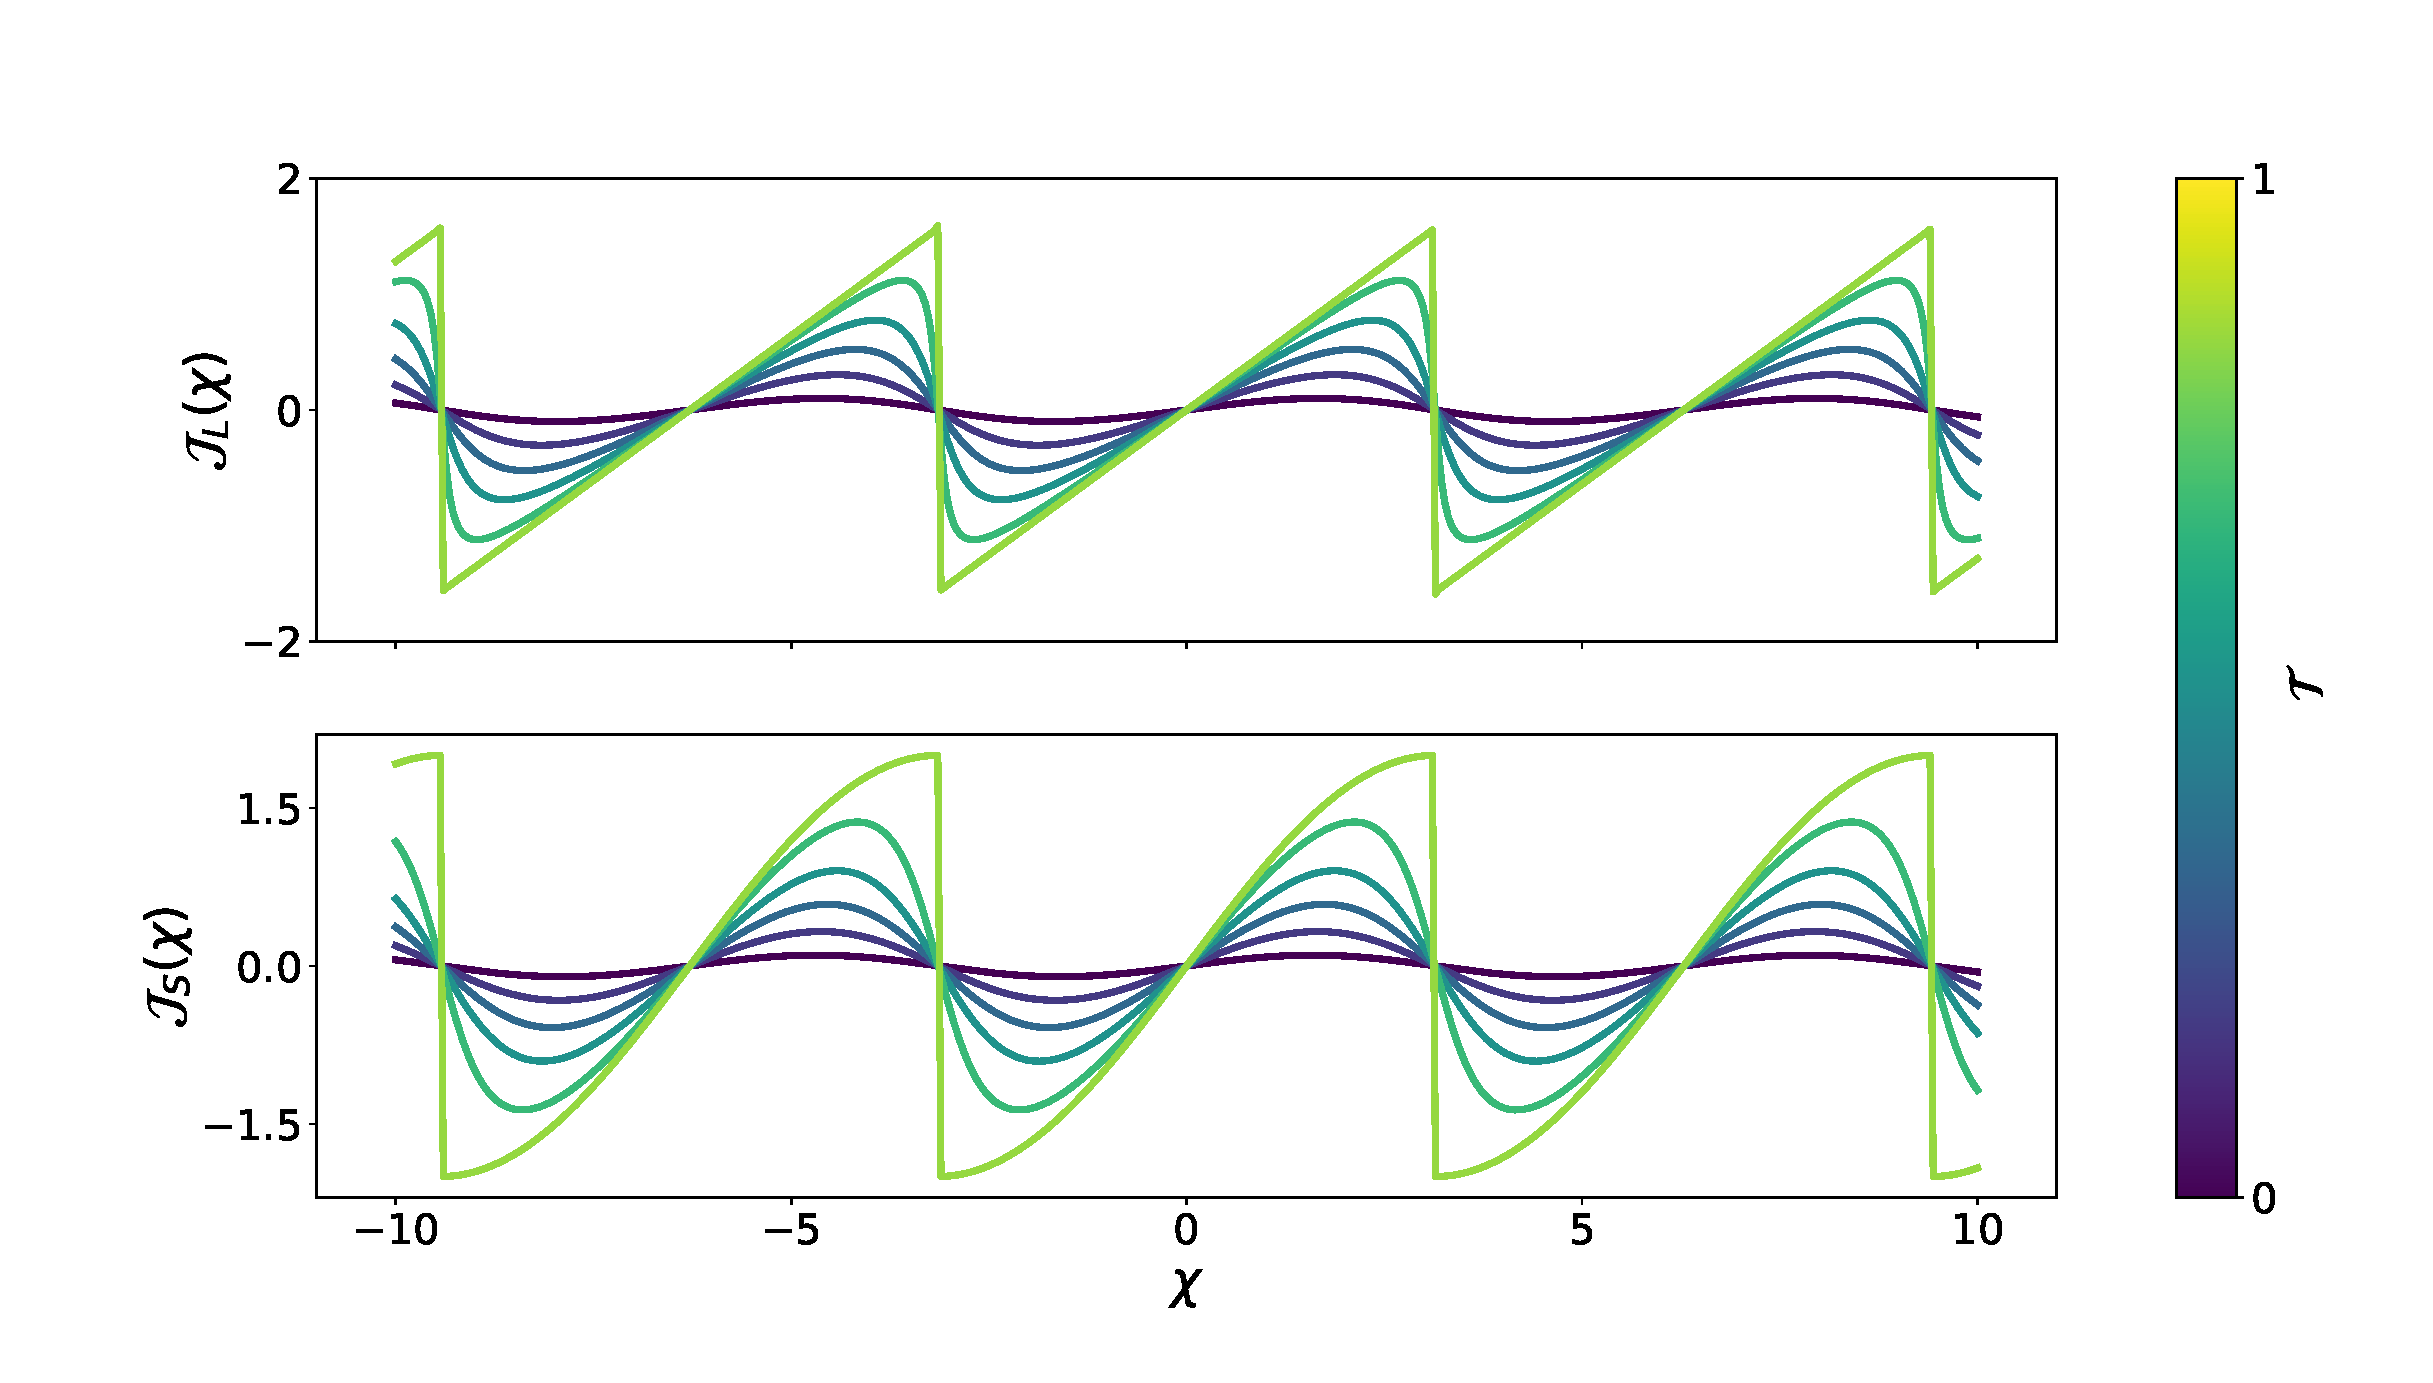
\includegraphics[width=\textwidth]{figure/analyticalmodel/current_density_all}
\caption{Current density plotted against the superconducting phase difference $\chi = \chi_2 - \chi_1$. The density from eq. (\ref{eq:long-j}) gives the sawtooth like shape for $\mathcal{J}^l$ for high values of $\mathcal{T}$. In the short junction limit, $\mathcal{J}^s$ holds from eq. (\ref{eq:short-j}). For low values of the transmission coefficient $\mathcal{T}$, both current densities look similar (sinusoidal form). }
\label{fig:current_density}
\end{figure}
Figure \ref{fig:current_density} shows a plot of both short and long junction limit current densities. For $\mathcal{T} \ll 1$, $\mathcal{J}^s$ takes a sinusoidal form, which also true for the long junction limit. For each of those, the classical Josephson relation can be found in the limit of low transmissions:
\begin{equation}
\mathcal{J} \simeq \mathcal{T} \sin \chi \label{eq:josephson-low-t}
\end{equation} The current densities differ for a large transmission coefficient $\mathcal{T} \simeq 1$: A sawtooth-like shape is observed in the long junction limit, and in the short junction limit, a sinusoidal shape appears.\\

%%%%%
\subsection*{Including magnetic field}
Up to this point, the current has been derived for zero magnetic field. If a finite magnetic field is considered, the phase $\chi$ is modified because of two effects: First, the magnetic phase that will be acquired along a trajectory connecting two points $y_1$ and $y_2$  leads to an additional term in the phase. Also, the superconducting phases at each interface become functions of $y_{1/2}$ (see \cite{Meier2016}):
%Then again, \textit{the condition of zero screening current in the bulk superconducting region and the limit of} $\lambda_L \rightarrow 0$ \textit{require the superconducting phase at the interfaces to become functions of y.
\begin{eqnarray}
\chi_{1/2} &=& \mp \frac{1}{2}\left( \chi - \frac{2 \pi B L }{\phi_0} y_{1/2}\right) \\
\tilde{\chi}(y_1, y_2) &=& \chi_2 - \chi_1 \\
 &=& \chi - \frac{\pi B L}{\phi_0}(y_1 + y_2)
 \label{eq:chi}
\end{eqnarray}
Assuming that the London penetration depth is small to zero in the superconducting regions, the following gauge for the vector potential can be used:
\begin{equation}
\mathbf{A}=A_y \mathbf{e}_y, \quad
A_y=\left\{ 
		\begin{array}{ll}
				-B x, & -L/2 \leq x \leq L/2, \\[0.2cm] 
				-\frac{1}{2} B L |x| , & \quad |x|>L/2
		\end{array} 
	\right.
\label{eq:Ay}
\end{equation}
This gauge will give no additional contribution to the phase on straight trajectories
\begin{eqnarray}
\delta \chi &=& \frac{2 \pi}{\Phi_0} \int d \mathbf{l} \cdot \mathbf{A} \\
&=& \frac{2 \pi}{\Phi_0} \int_{-L/2}^{L/2} \frac{dx}{\cos \theta} A_y (x) \sin \theta \\
&=& - \frac{2 \pi B}{\Phi_0} \frac{y_2 - y_1}{L} \int_{-L/2}^{L/2} x dx \\
&=& 0, \label{eq:magnetic-phase-straight}
\end{eqnarray}
where eq.~(\ref{eq:parametrization}) has been used. The total phase for this setup is therefore eq.~(\ref{eq:chi}). This results in the current phase relation in the expression for the Josephson current from eq. (\ref{eq:josephson_current_zero_b}) to be replaced by the effective phase $\chi \rightarrow \tilde{\chi}(y_1, y_2)$:
\begin{equation}
J\left(\chi, \phi \right) = \frac{2 e v_F}{\pi \lambda_F L^2}  \int \int_{-W/2}^{W/2} d y_1 d y_2 \frac{\mathcal{J}(\tilde{\chi}(y_1, y_2))}{\left[ 1 + \left(\frac{y_1 - y_2}{L}\right)^2\right]^2}
\label{eq:josephson_current}
\end{equation}
The critical current can be found by maximizing the Josephson current with respect to $\chi$:
\begin{equation}
I_c(\phi) = \text{max}_{\chi}\left\{ J(\chi, \phi) \right\}.
\end{equation}
The integation over $y_1$ and $y_2$ has been evaluated in \textbf{TODO cite!} yields the critical current
\begin{equation}
I_c(\chi) = \frac{2e W v_F }{\lambda_F L}\frac{( 1- \{ \phi \}) \{ \phi \} }{|\phi|} 
\end{equation}

\begin{figure}
\centering
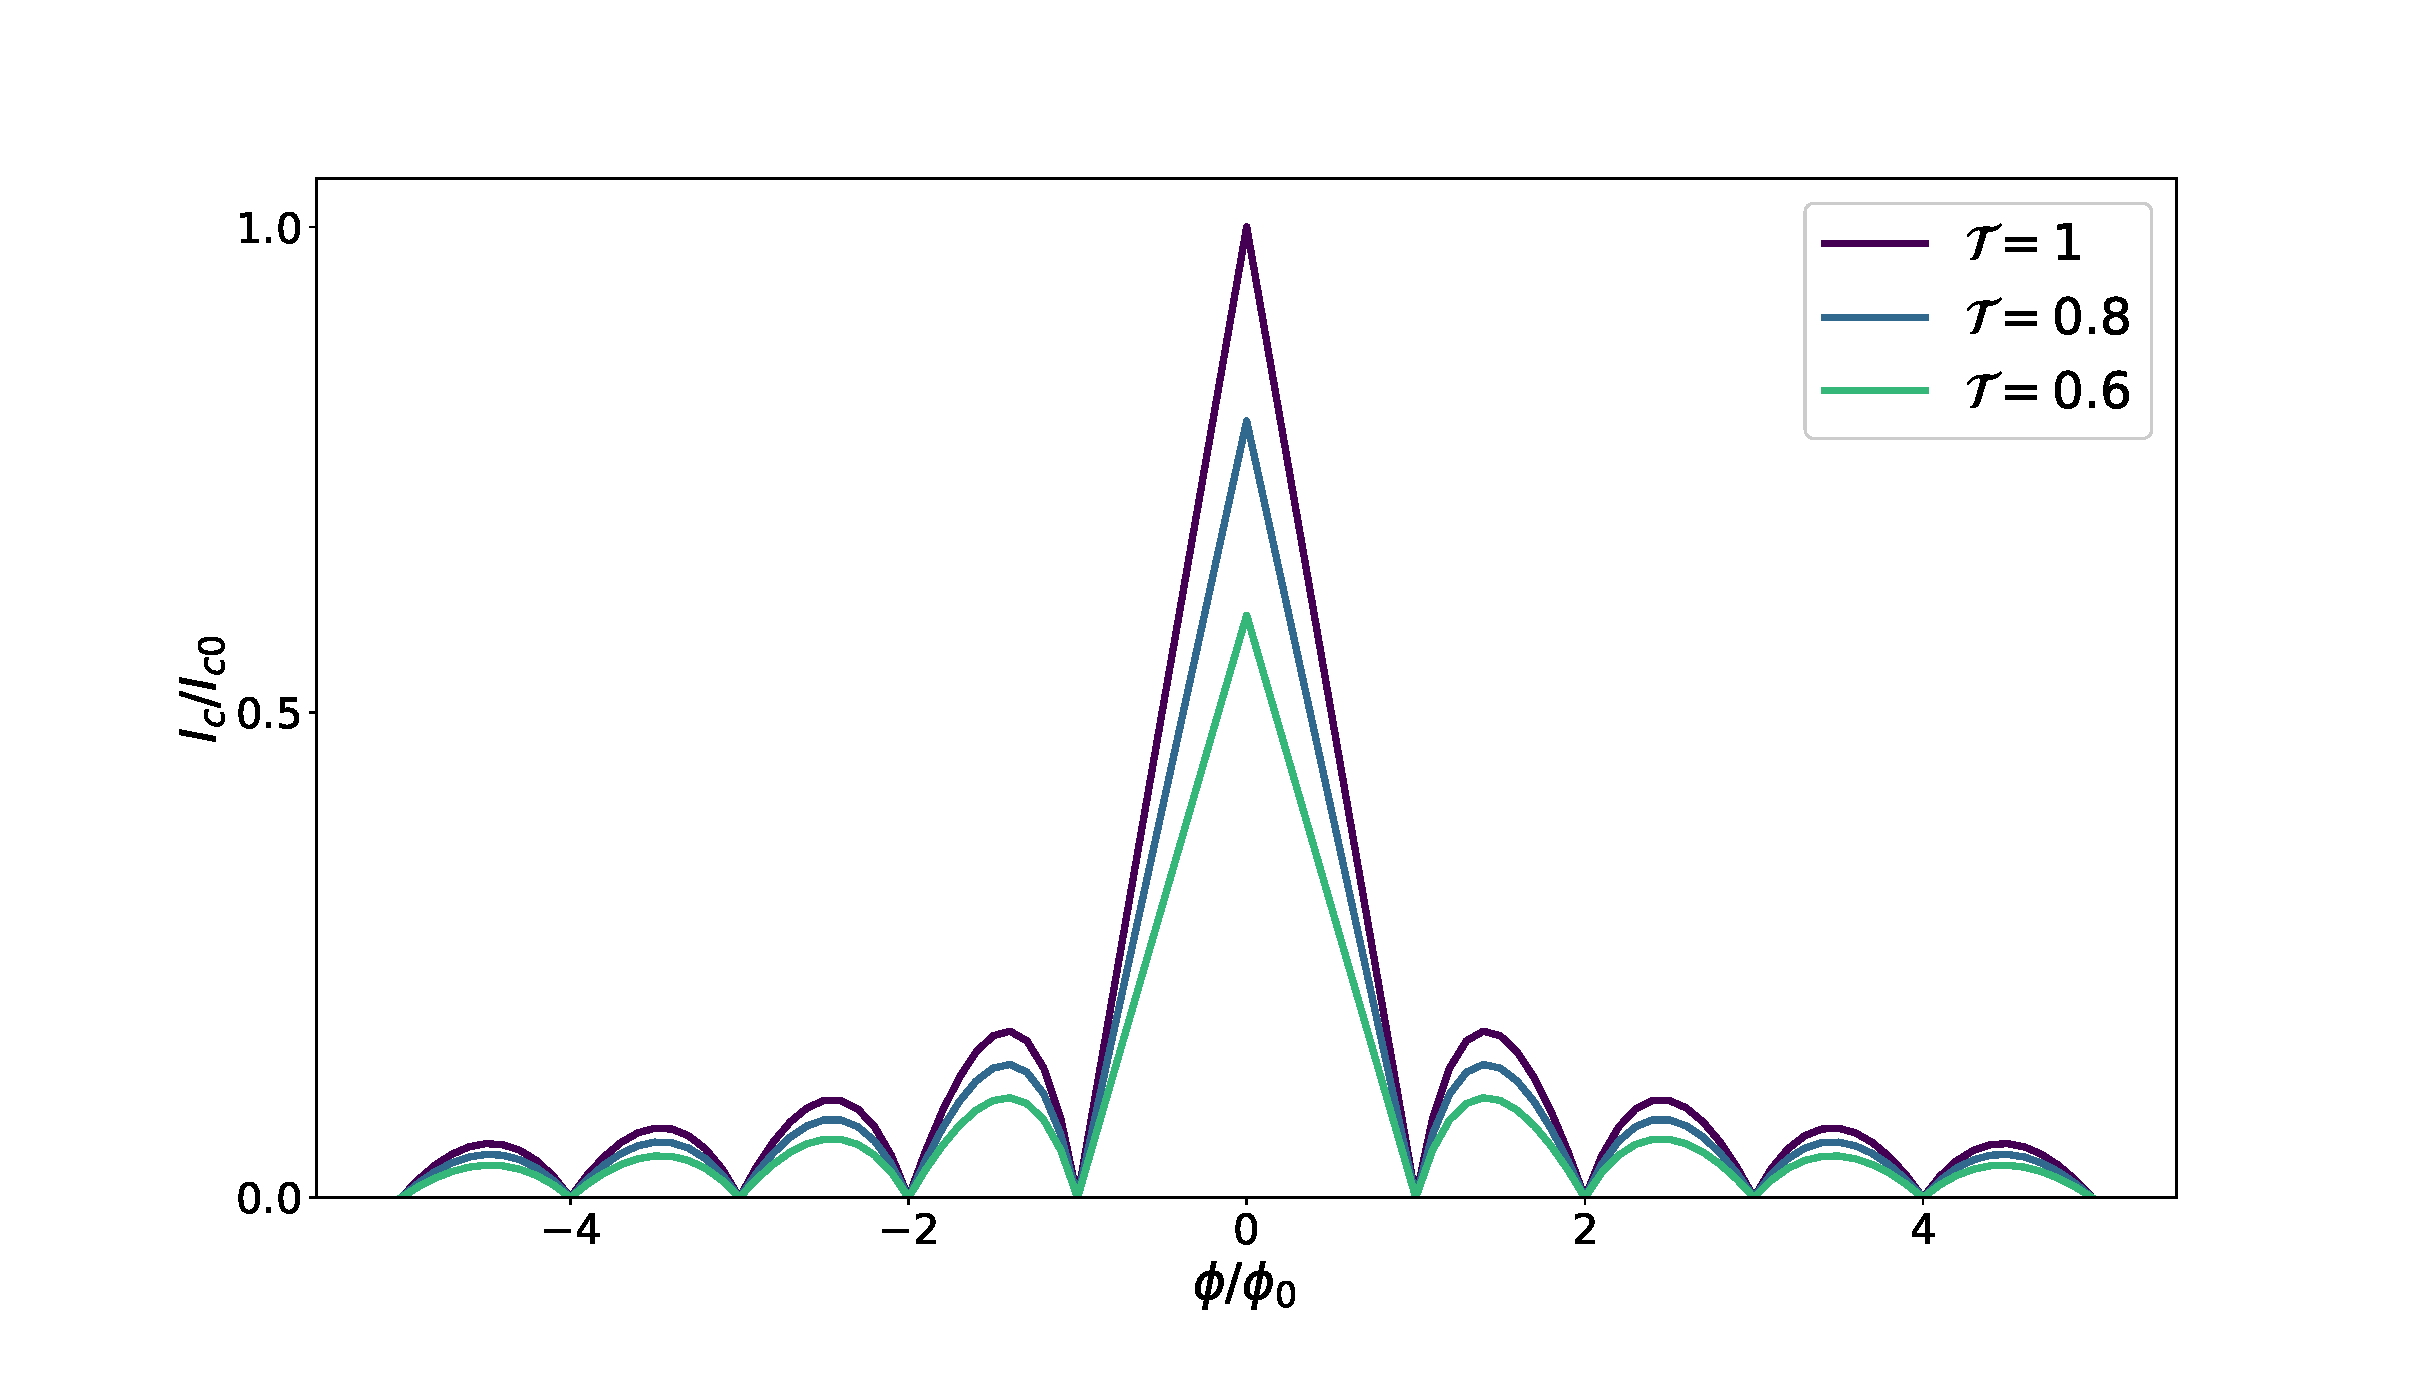
\includegraphics[width=0.8\textwidth]{figure/analyticalmodel/ic_vs_tau}
\caption{$I_c$ vs. $\phi$ for different values of  $\mathcal{T}$}
\end{figure}

\subsection*{Including scattering at the boundaries}

So far, straight trajectories connecting the two superconducting interfaces have been considered. A process that is possible in principal, is a trajectory of an electron that is scattered at a side boundary (see figure \textbf{TODO!}). It is clear that, especially in the case of a short and wide junction with $W \gg L$, these trajectories do not contribute as much as the straight trajectories. When a trajectory is scattered at, say, a point at the upper edge $(x, y) = (x_s, p W/2)$, the parametrisation for the angle describing the trajectory is
\begin{equation}
\tan \theta = \frac{\bar{y}_2 - y_1}{L} = \frac{W - y_2 - y_1}{L}. \label{eq:angles-scattering}
\end{equation}
In this parametrisation, the coordinate $\bar{y}_2$ is the mirror image of $y_2$. For straight trajectories the vector potential $\mathbf{A}$ does not give an additional contribution, which can be seen in eq. (\ref{qe:magnetic-phase-straight}). The effective phase is in this case determined by eq. (\ref{eq:chi}). When considering the scattering at side boundaries with the parametrization from eq. (\ref{eq:angles-scattering}), the contribution from the magnetic phase is no longer zero,
\begin{eqnarray}
\delta \chi &=& \frac{2 \pi}{\Phi_0} \int_{-L/2}^{x_s} dx A_y(x) \tan \theta  - \frac{2 \pi}{\Phi_0} \int_{x_s}^{+L/2} dx A_y(x) \tan \theta \\
&=& - \frac{2 \pi B }{\Phi_0 } \tan \theta \left( \int_{-L/2}^{x_s} x dx - \int_{x_s}^{+L/2} dx \right) \\
&=& - \frac{2 \pi B}{\Phi_0 } \tan \theta \left( x_s^2 - (L/2)^2 \right) \\
&=& ~ \frac{\pi \phi}{2 W} \frac{(W - 2 y_1) ( W - 2y_2)}{W - y_1 - y_2},
\end{eqnarray}
since the trajectory changes the direction and therefore $d \mathbf{l} \cdot \mathbf{A}$ changes sign. The total effective phase difference is then, using eq. (\ref{eq:chi})
\begin{equation}
\tilde{chi} (y_1, y_2) = \chi - \frac{\pi \phi}{2 W} \left( 2 (y_1 + y_2) - \frac{(W-2y_1)(W-2y_2)}{W - y_1 - y_2} \right)
\end{equation}
With the contribution from side boundary scattering, the total Josephson current is
\begin{equation}
J \left( \chi, \phi \right) = J^{(0)} \left( \chi, \phi \right)  + 2 J^{(1)} \left( \chi, \phi \right).
\end{equation}
$J^{(0)}$ denotes the part coming from straight trajectories. Since there are two side boundaries, the part describing the scattering, $J^{(1)}$, has an additional factor 2 and reads
\begin{equation}
J^{(1)} = \frac{2 e v_F}{\pi \lambda_F L^2} \int \int_{-W/2}^{W/2} \frac{d y_1 d y_2}{ \left[ 1 + \left(\frac{y_1 - y_2}{L}\right)^2\right]^{2}} \mathcal{J} \left( \chi - \frac{\pi \phi}{2 W} \left( 2 (y_1 + y_2) - \frac{(W-2y_1)(W-2y_2)}{W - y_1 - y_2} \right)\right)
\end{equation}
This contribution has not been noted in \cite{Meier2016}. In the case of short and wide junctions, it is sufficient to consider only $J^{(0)}$. For the cases, when $W / L \simeq 1$, it is necessary to sum over all possible edge channels.


\section{Calculation of QPC current}
\begin{figure}
\centering
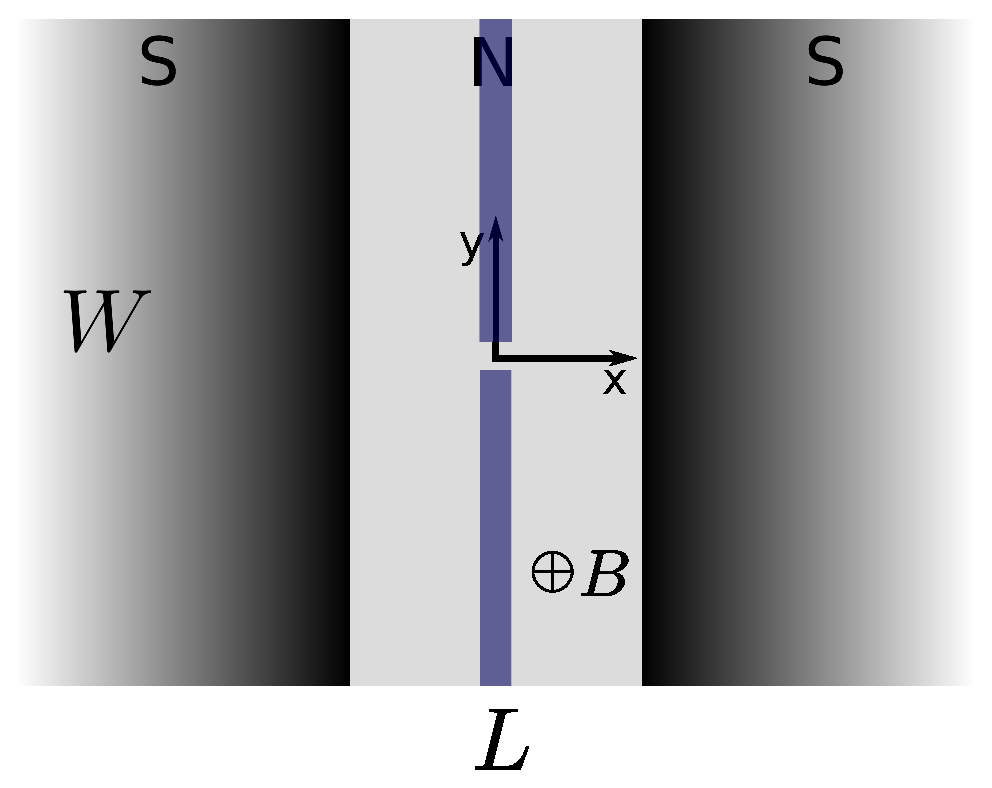
\includegraphics[width=0.5\textwidth]{figure/analyticalmodel/qpc_sns_junction}
\caption{SNS junction with a QPC gate on top. The split is located at $(x, y) = (0, 0)$ and the width of the barrier is assumed to be negligible. Each trajectory that contributes has to pass though the origin. The angles $\theta_1$ and $\theta_2$ parametrize this trajectory.}
\label{fig:qpc_sns_schematic}
\end{figure}
%\textbf{TODO: what happens when a constriction is on top of normal layer, fermi levels etc}
The quasi classical formalism can even be employed to modified SNS junctions. One can build gates on top of the normal region of the junction in a way that the current cannot pass through the gated regions (see chapter \ref{ch:experiment}). In the quasi classical picture, this means that the possibilities for trajectories connecting two points at the superconducting interfaces are limited through the geometry of the constriction.\\
Figure \ref{fig:qpc_sns_schematic} shows a sketch of the quantum point contact set-up which will be analysed with the quasi classical formalism. The normal region of the SNS junction is covered by a gate with a small split in the middle. The split is located at $(x, y) = (0, 0)$ so that the sample is symmetric around the origin. The width of the split is in the order of $\lambda_F$  and can thereby be viewed as an isotropic scattering point with transmission coefficient $\mathcal{T}_0$. Trajectories connecting the two superconducting interfaces have to pass through the QPC. For simplicity, the geometrical width of the barrier is neglected, only straight trajectories are considered, and scattering at side edges is neglected. This modified set-up leads to a different parametrization of the trajectories and therefore to a different magnetic phase than in eq. (\ref{eq:chi}).\\
With the QPC set-up, all possible trajectories are parametrized by two angles $\theta_1$ and $\theta_2$. $\theta_1$ describes the trajectory before passing through the QPC in the region $ -L/2 < x < 0$, and  $\theta_2$ after passing through the QPC. The parametrization of the trajectories reads
\begin{equation}
\tan \theta_1 = - \frac{2 y_1}{L}, \quad \tan \theta_2 = \frac{2 y_2}{L}
\label{eq:QPCparametrization}
\end{equation}
With the gauge from eq. (\ref{eq:Ay}), the magnetic phase acquired within the sample reads
\begin{eqnarray}
\frac{2\pi}{\Phi_0} \int d\mathbf{l} \cdot \mathbf{A}  &=&
-\frac{\pi B}{\Phi_0}\left(\frac{L}{2}\right)^2
\left(-\tan\theta_1 + \tan\theta_2\right) =
-\frac{\pi \phi (y_1+y_2)}{2 W}.
\label{eq:phaseQPC}
\end{eqnarray}
The total phase difference is the difference of the contribution coming from the magnetic field, eq. (\ref{eq:phaseQPC}) and the supcondcucting phase difference eq.~(\ref{eq:chi}). The effective phase for the QPC setup is found to be
\begin{equation}
\tilde{\chi}(y_1,y_2)=\chi-\frac{ \pi \phi }{2W}(y_1+y_2).
\label{eq:chiQPC}
\end{equation}
%The contribution in eq. (\ref{eq:chiQPC}) is half of the effective phase without any constriction, as written in eq. (\ref{eq:chi}). This is reasonable and can be illustrated by looking at the area contributing to the phase. Only half of the normal region is covered by all possible trajectories in the QPC case, whereas in the case without any constriction, the whole normal region contributes.\\
%\textbf{TODO: stimmt das da oben? warum?}\\
One consequence of the additional gate on top of the normal region is the change in the effective phase, resulting in a modified current phase relation $\mathcal{J}(\tilde{\chi}(y_1, y_2))$. Another consequence is a modified expression for the critical current. In the set-up without gates, straight trajectories with a fixed angle $\theta$ were considered and summed up to a total contribution. The difference in the QPC set-up is the split in the gate, which is modelled as an isotropic scattering point. The trajectories being summed up in this set-up can be thought to consist of two parts. The first part connects $y_1$ with the split at $(x, y) = (0, 0)$ and is determined by the direction of the trajectory. This explains the Fermi velocity in this part(?). The second part of the current trajectory starts from the origin and connects it with a point at the right interface $y_2$. Summing up, the  critical current in the QPC set-up is
\begin{equation}
I_c^{\text{QPC}}(\phi) \propto \text{max}_{\chi} \int d \theta_1 v_F \cos^2 \theta_1 \int d \theta_f \cos \theta_f \mathcal{J}\left( \tilde{\chi} (\theta_1, \theta_2) \right)
\end{equation}
%The normalized critical current reads
%\begin{eqnarray}
%\frac{I_c(\phi)}{I_c(0)} &=& \frac{ \text{max}_{\chi} \int d \theta_i \cos^2 \theta_i\int d \theta_f \cos \theta_f \mathcal{J}(\tilde{\chi}(\theta_i, \theta_f)) }{ \text{max}_{\chi} \int d \theta_i \cos^2 \theta_i\int d \theta_f \cos \theta_f \mathcal{J}(\chi) }
%\end{eqnarray}
The QPC is modelled as an isotropic scatterer with transmission probability $\mathcal{T}$. If the transmission is small, $\mathcal{T} << 1$, eq.~(\ref{eq:josephson-low-t}) can be used for $\mathcal{J}$.
%TODO \textbf{TODO: add why from $\sin \tilde{\chi}$ only cosine survives!}
The angles $\theta_{1, 2}$ can be rewritten in terms of $y_{1, 2}$ by using the parametrization from eq.~(\ref{eq:QPCparametrization}), allowing the normalized critical current to be expressed as
\begin{eqnarray}
\frac{I_c(\phi)}{I_c(0)} &=& \frac{\mathcal{I}_2(\phi)\mathcal{I}_{3/2}(\phi)}{\mathcal{I}_2(0)\mathcal{I}_{3/2}(0)},
\end{eqnarray}
where the integrals $\mathcal{I}$ are defined as
\begin{equation}
\mathcal{I}_k(\phi) = \frac{2}{L}\int_{-W/2}^{+W/2}dy \frac{\cos\left(\frac{\pi\phi y}{2W}\right)}{\left[1 + \left(\frac{2y}{L}\right)^2 \right]^k}
\label{integral-qpc}
\end{equation}
\subsubsection*{Numerical evaluation}

Evaluating the integral numerically, one finds 

\begin{figure}
\centering
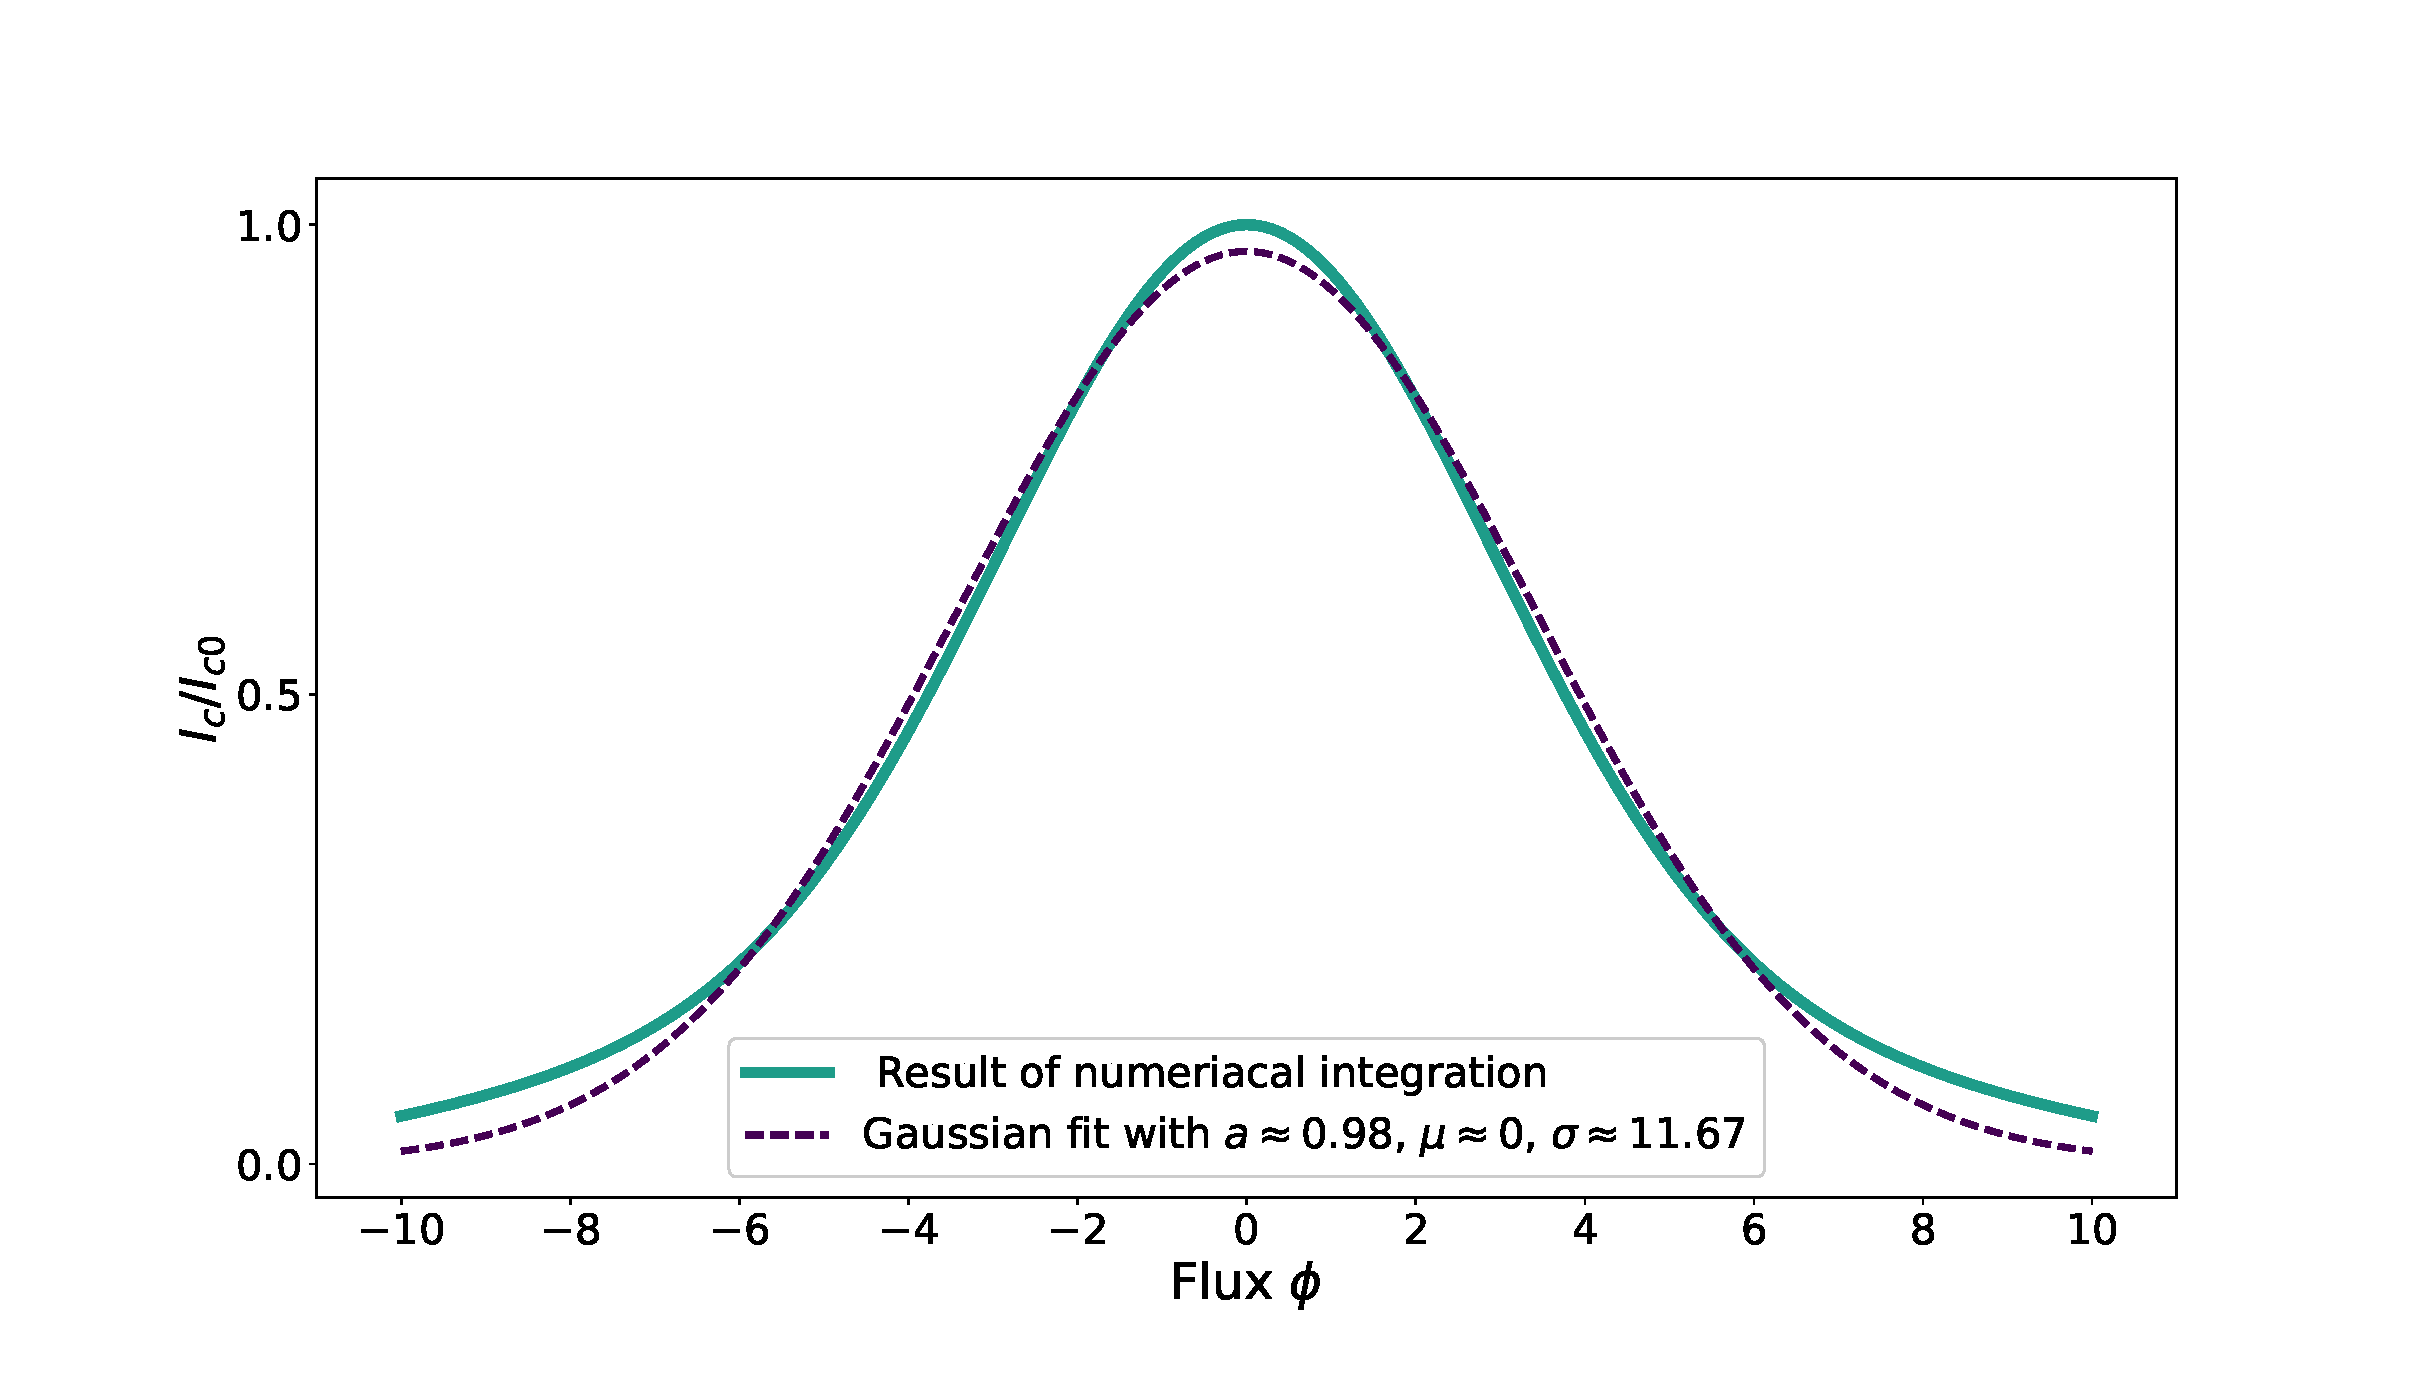
\includegraphics[width=0.6\textwidth]{figure/analyticalmodel/qpc-numerical-integration-fit}
\end{figure}
\subsubsection*{Evaluation in limits}
The current can be evaluated in the limit of small flux $\phi \rightarrow 0$, and in limit of high fields $\phi \rightarrow \infty$. 
At $\phi=0$ the cosine term becomes one leading to the simple expression
\begin{eqnarray}
\mathcal{I}_2(0)\mathcal{I}_{3/2}(0) &=&
\frac{2 W^2 L}{\left( L^2 + W^2 \right)^{3/2}} + \frac{2W}{\sqrt{L^2 + W^2}} \arctan \frac{W}{L}  \\
&\equiv & \frac{2 x^2}{\left( 1 + x^2 \right)^{3/2}} + \frac{2 x}{\sqrt{1 + x^2} } \arctan x,
\label{Ic-0}
\end{eqnarray}
where $x \equiv W/L$.
The parabolic asymptotics of the critical current at small $\phi$ is found by expanding the cosine factors in the numerator:
\begin{eqnarray}
\frac{I_c(\phi)}{I_{c0}}&\simeq& 1 - \frac{\pi ^2 \phi^2 }{32} f_0(W/L) \\
f_0(x) &=& \frac{\sqrt{x^2+1} \log \left(\sqrt{x^2+1}+x\right)}{x^3} - \frac{2}{x (x+(x^2+1) \arctan x)} 
\end{eqnarray}
In the opposite limit of high fields, $\phi\to \infty$, the integration in eq.~(\ref{integral-qpc}) is extended over $y_1$ and $y_2$ to $\pm \infty$ and obtain
\begin{eqnarray}
\frac{I_c(\phi)}{I_{c0}} &=& \frac{\pi^{3/2}}{8 x} \frac{(1 + x^2)^{3/2}}{x + (1+x^2) \arctan x} \left( \frac{\pi \phi}{2 x} \right)^{3/2} \exp \left( - \frac{\pi \phi}{2 x} \right)
\label{eq:large-phi}
\end{eqnarray}
%\textbf{TODO: write this one in pretty}
\newpage
\section{QPC edge current}
Additionally to the QPC, two edge channels at $(x, y) = (0, \pm w/2)$ are introduced. The QPC is modelled with the transmission coefficient $\mathcal{T}_q$, and the edge channel with the coefficient $\mathcal{T}_e$. The lattice orientation of the graphene structure may may be either predominantly arm-chair or zigzag. Depending on this orientation, the edge currents may or may not contribute significantly  to the total current. The Fraunhofer pattern changes accordingly.
%TODO cite!
\begin{figure}
\centering
\includegraphics[width=0.5\textwidth]{figure/analyticalmodel/qpc_edges_angles}\label{fig:qpc-edge-parametrization}
\caption{A SNS junction with split at upper edge, $(x, y) = (0, + W/2)$. Similar to the QPC set-up, this constriction is formed in a way that each trajectory has to pass through to contribute to the current.}
\end{figure}
The parametrization of an edge trajectory, illustrated in figure \ref{fig:qpc-edge-parametrization}, reads
\begin{eqnarray}
\tan \theta_1 = ~\frac{ W - y_1}{L/2}, \quad \tan \theta_2 = -\frac{W - y_2}{L/2} \label{eq:angles-edge}.
\end{eqnarray}
Similar to the QPC contribution, the magnetic phase gain along the trajectory is calculated. For the upper edge, the result is
\begin{eqnarray}
\frac{2 \pi}{\phi_0} \int d \mathbf{l} \cdot \mathbf{A} &=& \frac{2 \pi}{\phi_0} \left( \int A_y(x) |d\mathbf{l}| |\mathbf{e_y}| \sin \theta_1 + \int A_y(x) |d\mathbf{l}| |\mathbf{e_y}| \sin \theta_2  \right)\\
%&=& \frac{2 \pi B}{\phi_0} \left( \int_{-L/2}^{0} \frac{x dx}{\cos \theta_1} \sin \theta_1  + \int_{0}^{L/2} \frac{x dx}{\cos \theta_2} \sin \theta_2 \right) \\
&=&  - \frac{2 \pi B}{\phi_0} \left( \int_{-L/2}^{0} x dx \tan \theta_1 + \int_{0}^{L/2} x dx \tan \theta_2 \right) \\
&=&  - \frac{\pi B}{\phi_0} \frac{L}{2} \left( - \tan \theta_1 + \tan \theta_2 \right) \\
&=& - \frac{\pi B}{\phi_0} \frac{L}{2} \left( -2W + (y_1 + y_2) \right)\\
&=& \pi \Phi -\frac{\pi \Phi }{2 W} (y_1 + y_2),
\end{eqnarray}
where
\begin{equation}
\Phi = \frac{\phi}{\phi_0}, \quad \phi = B W L
\end{equation}
has been used. Together with the contribution from the set-up without any constriction from eq.~(\ref{eq:chi}), the total phase for the edge transmission is added up to
\begin{equation}
\tilde{\chi}(y_1, y_2) = \chi - \frac{3 \pi \Phi}{2\phi_0} (y_1 + y_2) + \pi \Phi \label{eq:chi-edge}.
\end{equation}
This is the effective phase $\tilde{\chi}(y_1, y_2)$ for the upper edge. Analogously, the phase for the lower edge can be constructed with a simple sign change in the parametrization in eq. (\ref{eq:angles-edge}), leading to
\begin{equation}
\tilde{\chi}(y_1, y_2) = \chi + \frac{3 \pi \Phi}{2\phi_0} (y_1 + y_2) - \pi \Phi \label{eq:chi-edge}
\end{equation}
The Josephson relation for the edge contribution has the modified phase from eq. (\ref{eq:chi-edge}). 
The result for the QPC in the limit in high fields, eq. (\ref{large-phi}), has a transmission coefficient $\mathcal{T} = 1$. For easier comparison with the edge channel contribution, this is rewritten into the following form
\begin{equation}
I_c^{\text{QPC}} = \mathcal{T}_q F(W/L)
\end{equation},
where the function $F(W/L)$ represents the result from eq. (\ref{eq:large-phi}). The integrals for the upper edge can be written in a similar way:
\begin{eqnarray}
I_c^e &=& \mathcal{T}_e \sin \left( \chi_0 - \pi \Phi \right) \int_0^\infty d \tilde{y}_1 \int_0^\infty d \tilde{y}_2 \frac{\cos \left( \frac{3 \pi \Phi \tilde{y}_1}{2 W} \right) }{\left( 1 + \left( \frac{2 \tilde{y}_1}{L}\right)^2 \right)^2} \frac{\cos \left( \frac{3 \pi \Phi \tilde{y}_2}{2 W} \right)}{\left( 1 + \left( \frac{2 \tilde{y}_1}{L}\right)^2 \right)^{3/2}} \\
&=& \mathcal{T}_e \sin \left( \chi_0 - \pi \Phi \right) \frac{F(W/L)}{4}, 
\end{eqnarray}
where
\begin{equation}
\tilde{y}_{1/2} = W/2 - y_{1/2} 
\end{equation}
The total critical current though the junction is proportional to the sum of the individual contributions
\begin{eqnarray}
\frac{I_c\left( \phi \right)}{I_{c0}} &=& \text{max}_\chi \left\{ \mathcal{T}_q \sin \chi + \frac{\mathcal{T}_e}{4} \sin \left( \chi - \pi \phi \right) + \frac{\mathcal{T}_e}{4} \sin \left( \chi + \pi \phi \right) \right\} / \left( \mathcal{T}_q + \mathcal{T}_e/2 \right)\\
&=& \frac{\mathcal{T}_q / \mathcal{T}_e + \cos \left( \pi \phi \right)/ 2 }{\mathcal{T}_q / \mathcal{T}_e + 1/2}\label{eq:ratio-transmissions}
\end{eqnarray}
\begin{figure}
\centering
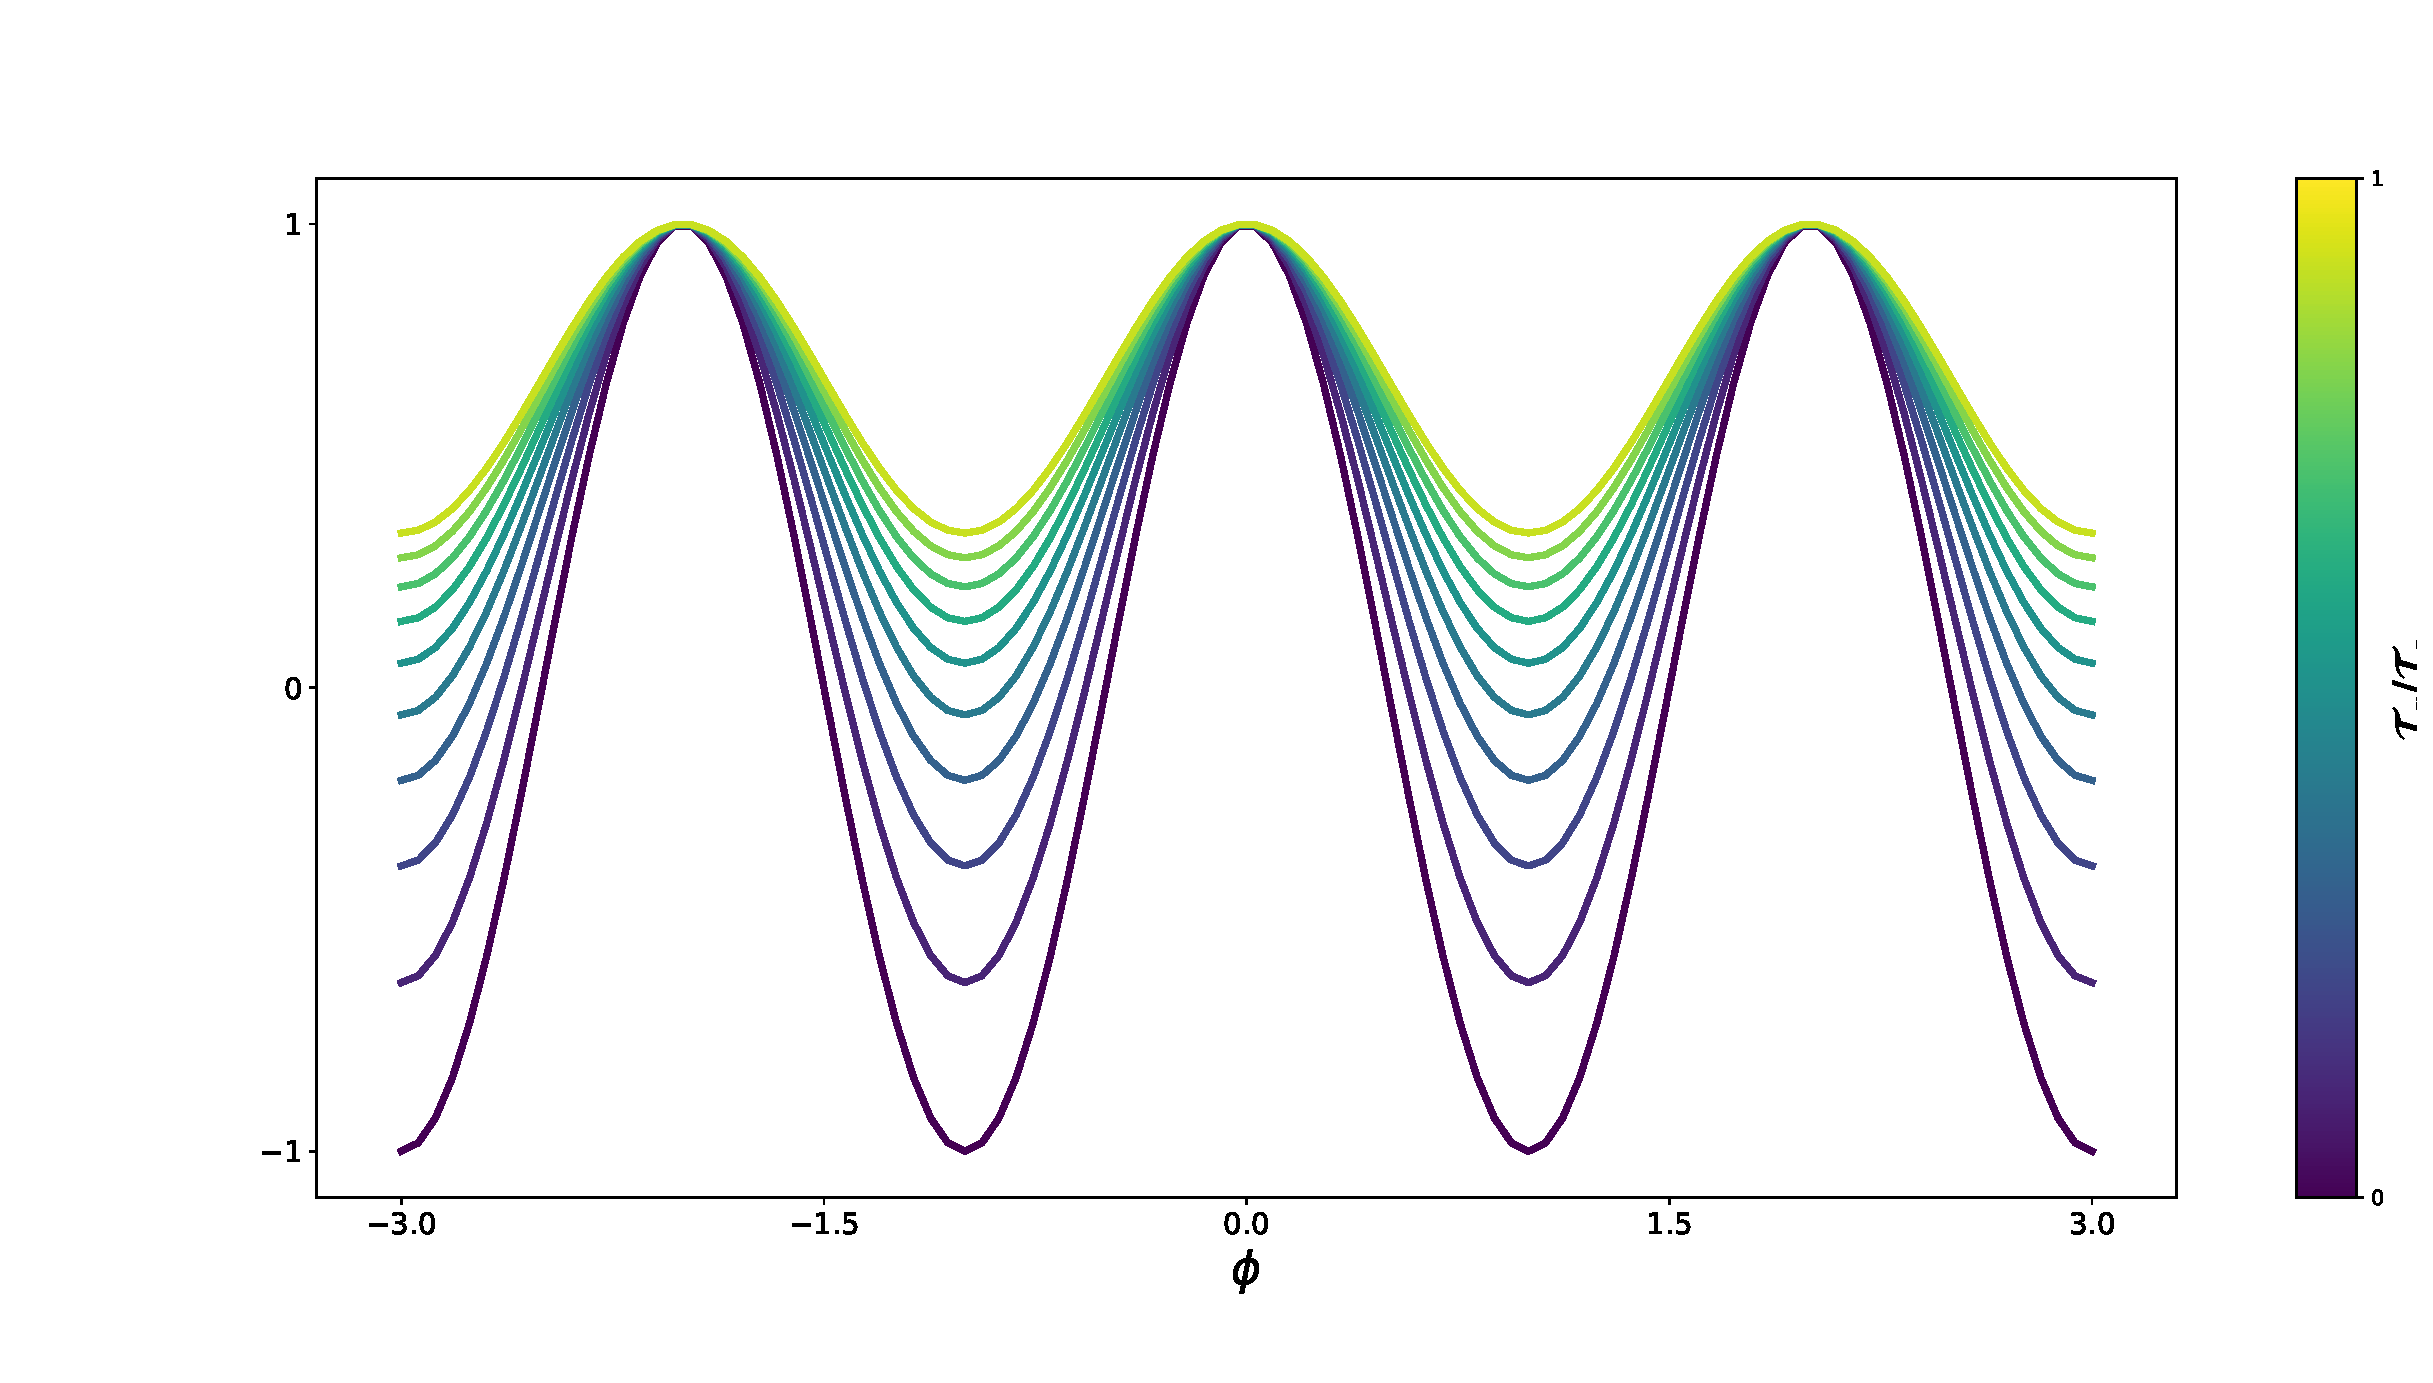
\includegraphics[width=\textwidth]{figure/analyticalmodel/ratio-transmissions} 
\caption{Another figure caption. Whatever.}\label{fig:ratio-transmissions}
\end{figure}
The result of eq. (\ref{eq:ratio-transmissions}) is plotted in figure \ref{fig:ratio-transmissions}. 
%For $\mathcal{T}_q/\mathcal{T}_e \ll 1$
\begin{figure}
\centering
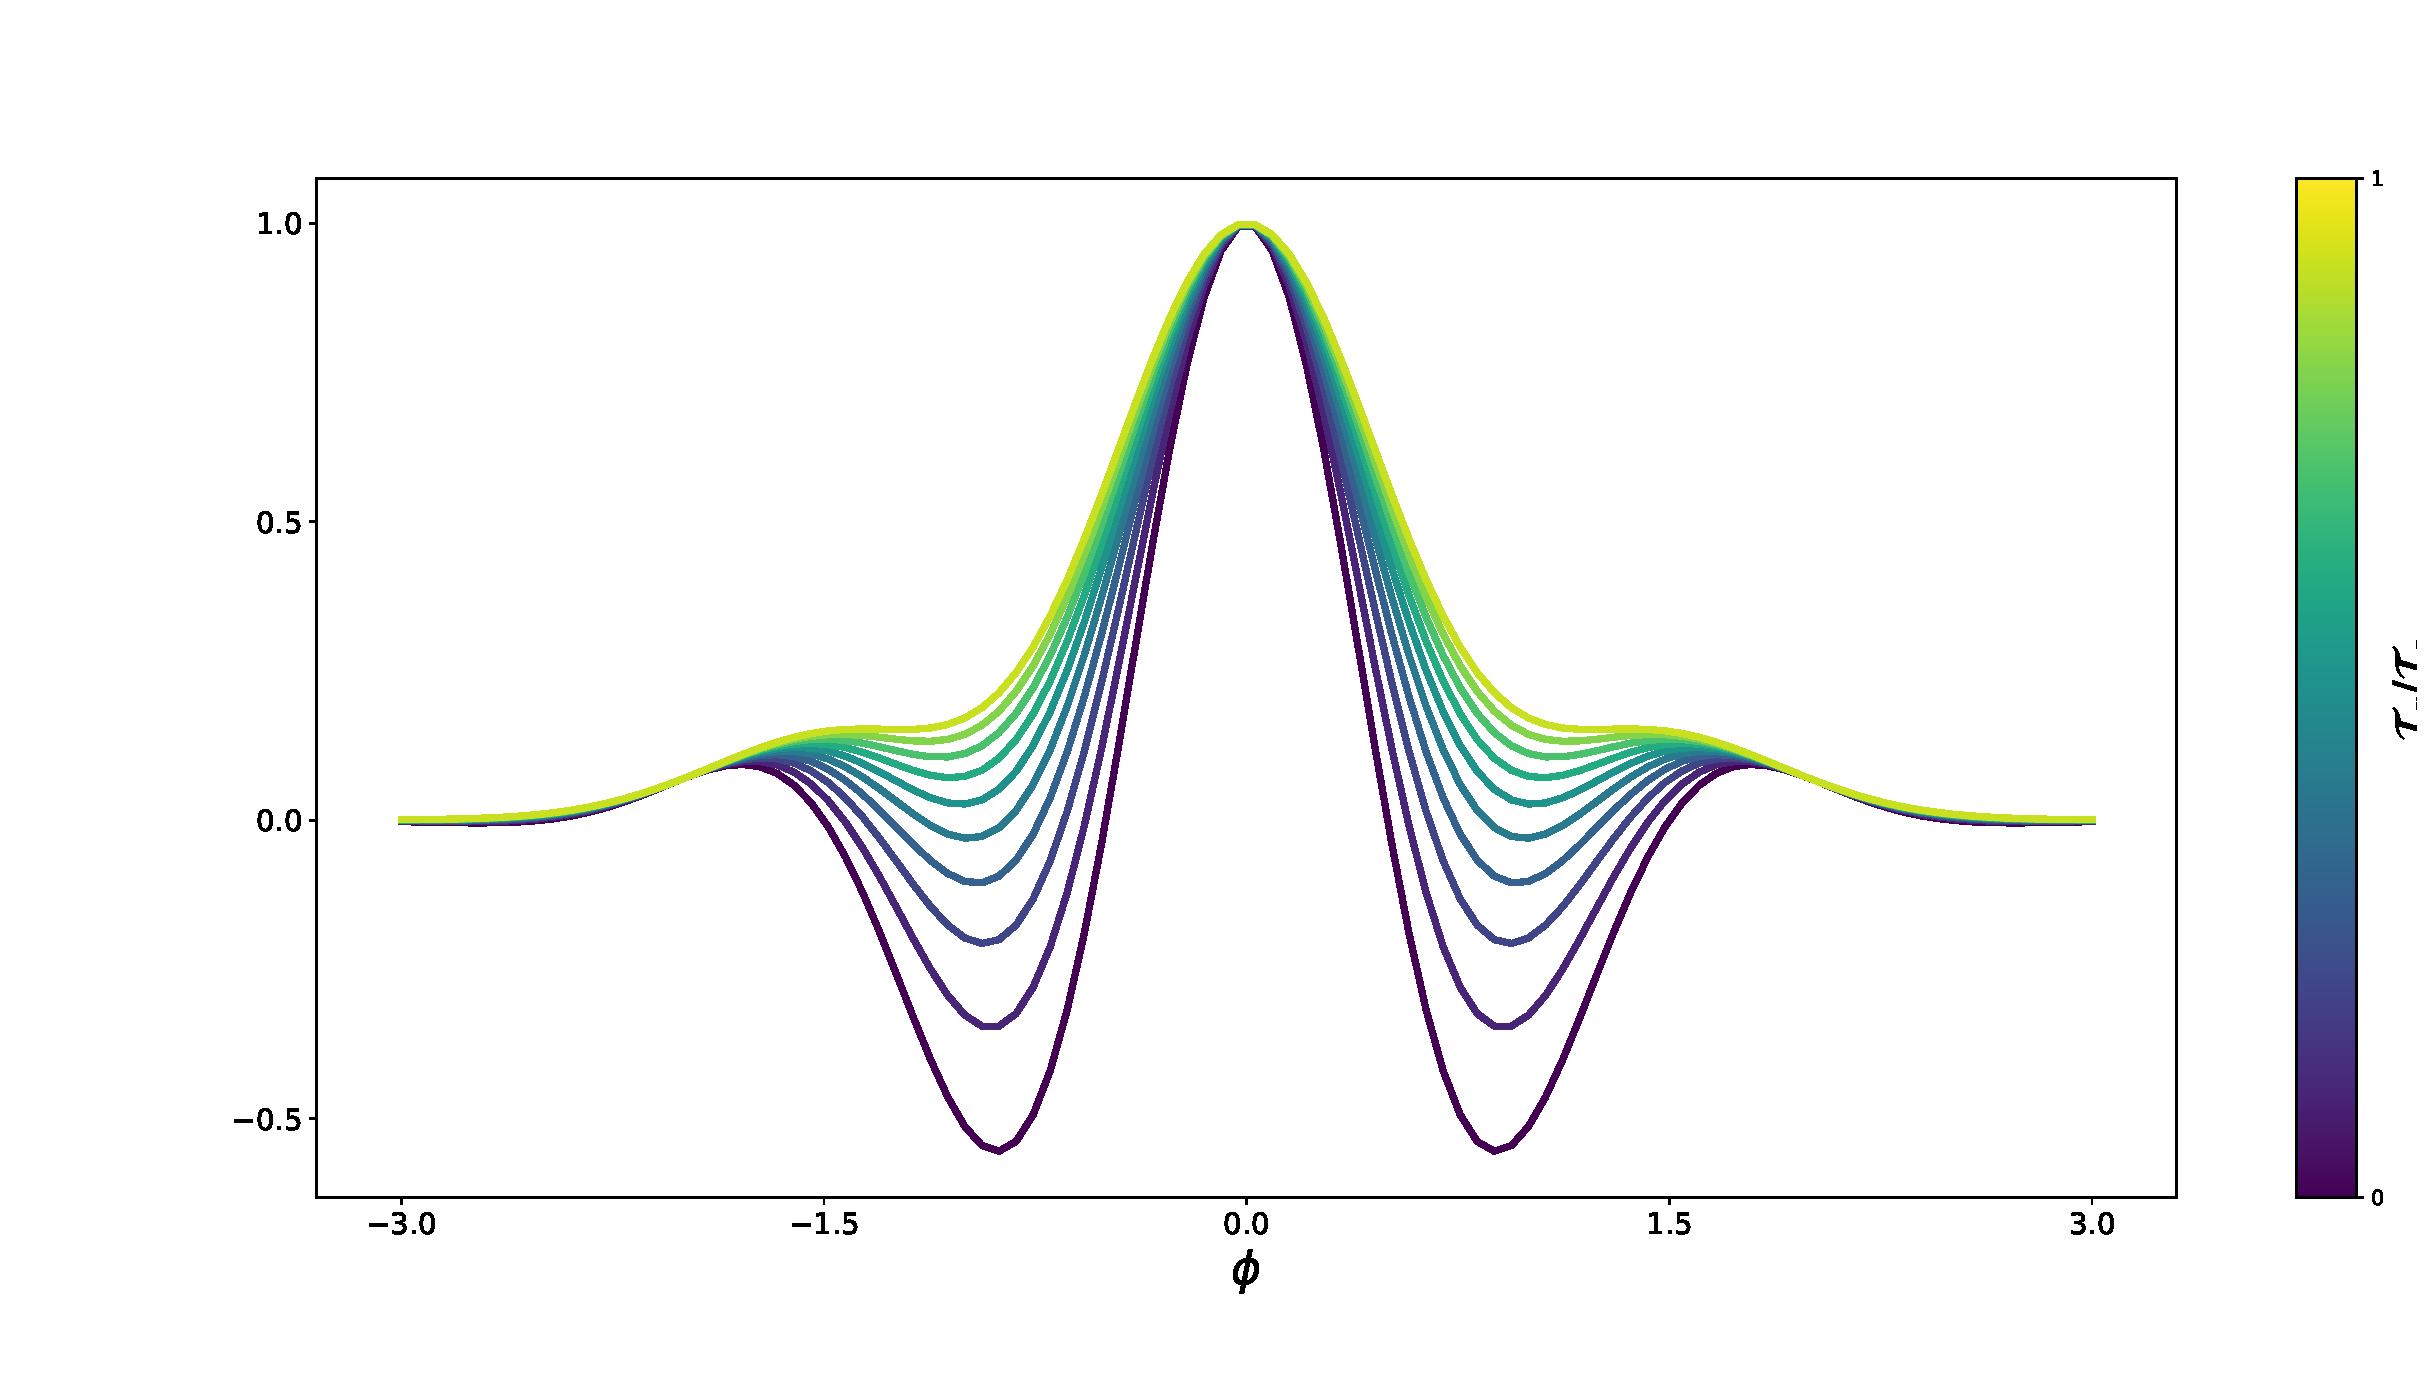
\includegraphics[width=\textwidth]{figure/analyticalmodel/ratio-transmissions-gaussian}
\caption{Some figure.}\label{fig:modulated-pattern}
\end{figure}
Figure \ref{fig:modulated-pattern} shows a plot of the ratio from eq. (\ref{eq:ratio-transmissions}) multiplied with a gaussian curve. 

\textbf{TODOs: \\
make plot colors uniform\\
add figure captions\\
check plots for edge current --> cbar seems wrong}
%write more about edge current contribution

\section{Barrier with finite split width - Transition to QPC setup}
\begin{figure}
\centering
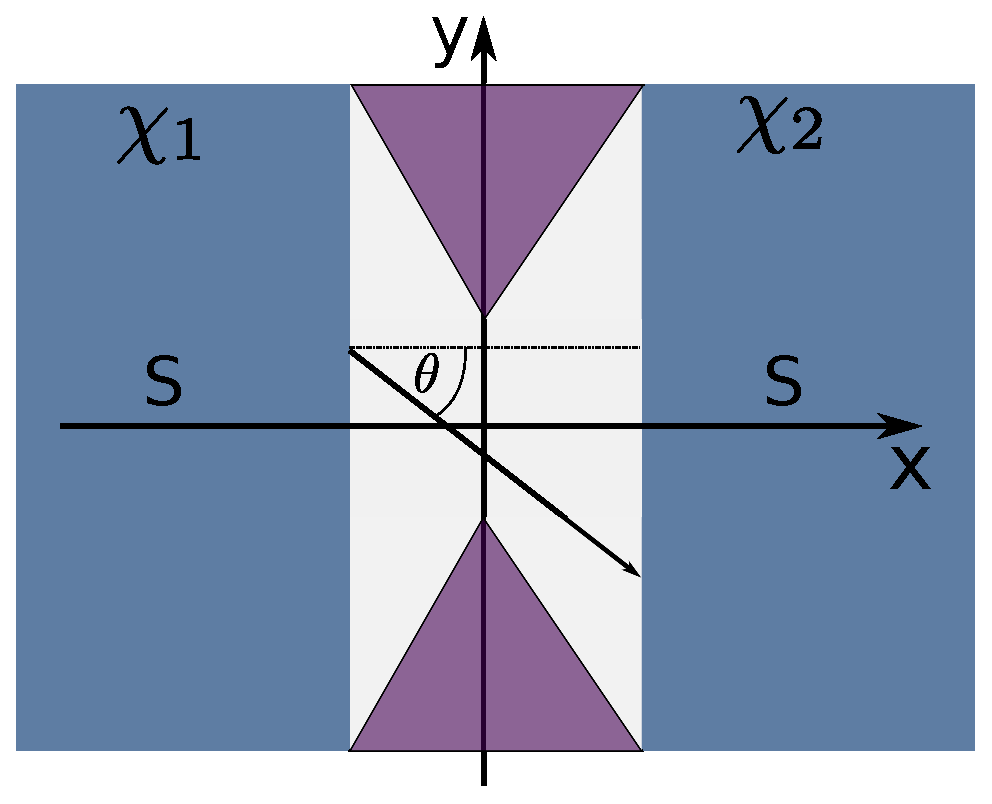
\includegraphics[width=0.5\textwidth]{figure/analyticalmodel/hourglass}
\caption{Hourglass setup}\label{fig:hourglass}
\end{figure}
The QPC setup and the SNS setup without barriers can be linked conceptually by investigating an hourglass-shaped setup. This setup constricts the trajectories through a split with a finite width $w_s$ and is visualized in figure (\ref{fig:hourglass}). When considering only straight trajectories, this split width models the transition to the QPC in the limit of $w_s \rightarrow 0 $. The difference to the QPC is simply the parametrization of the angles: with a finite $w_s$, trajectories are parametrized by only one angle $\theta$, the direction does not change after passing the split. When $w_s$ is small enough, like in the QPC case, two independent trajectories are considered with two parametrization angles $\theta_1$ and $\theta_2$. 
%TODO size of $w_s$?
This setup is particularly interesting because the impact of asymmetry in the junction can be studied. When relocating the split by for example moving it along the $x$-axis, the possible trajectories are limited. As a consequence, the Fraunhofer pattern changes. 
%TODO das ist ein bisschen dünn...

%TODO cite?

\chapter{Numerical Results}
\label{ch:numerical-results}
%\begin{figure}
%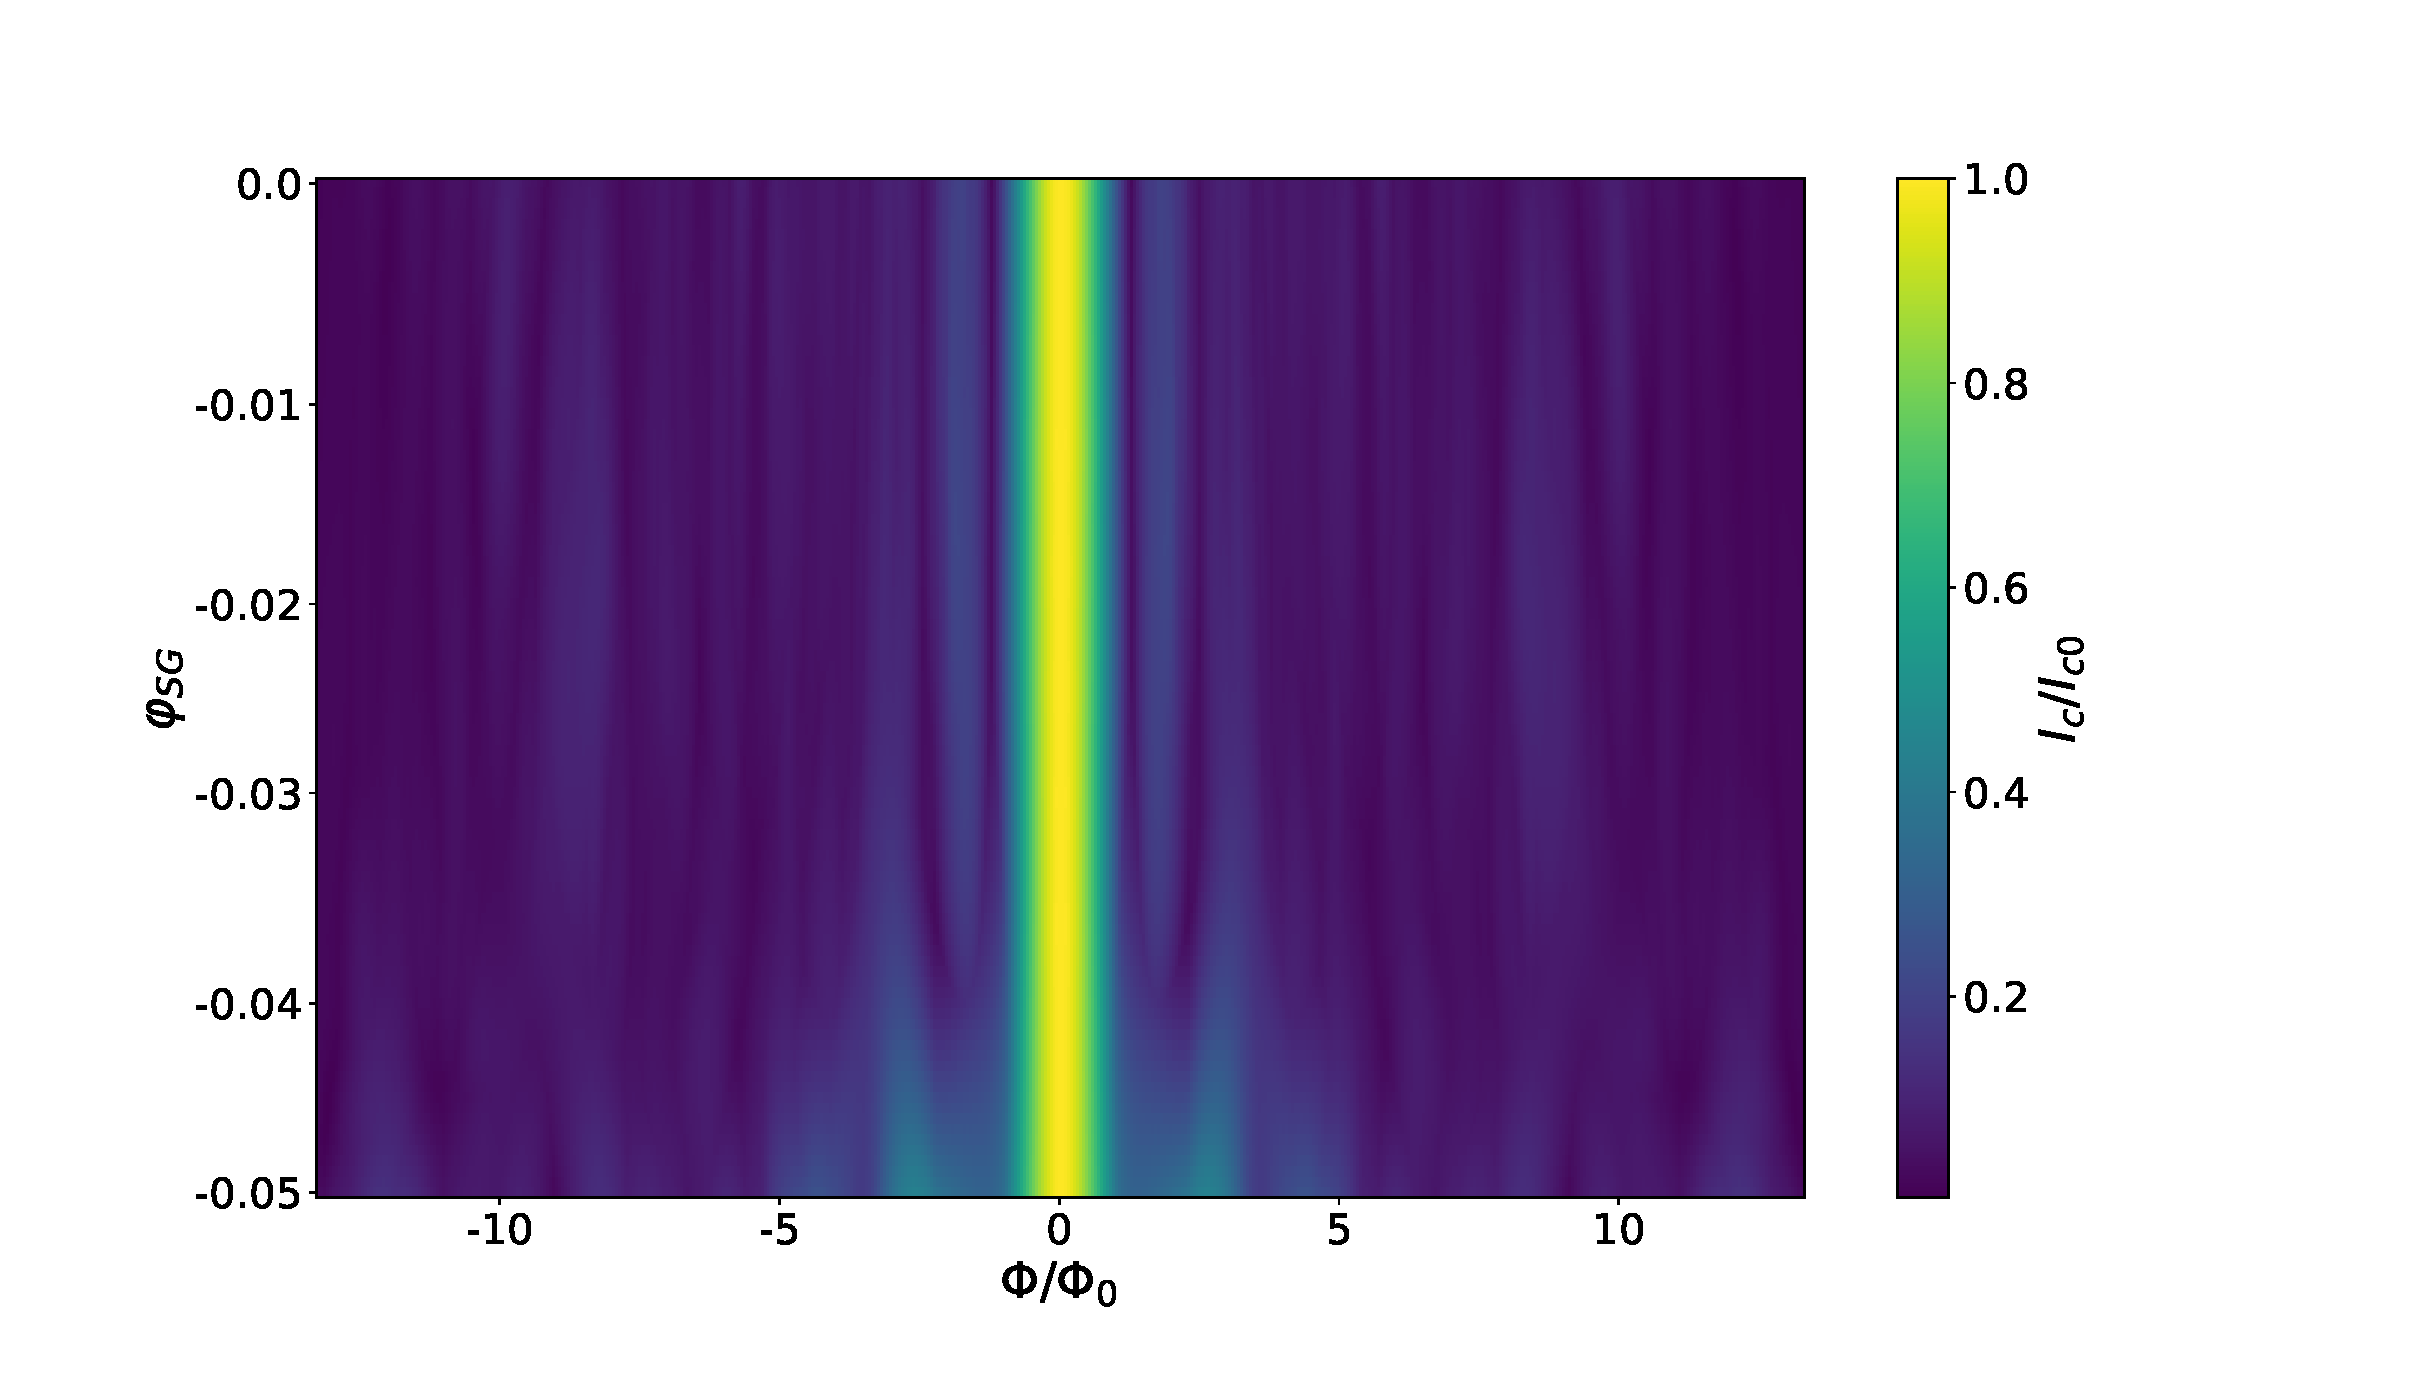
\includegraphics[width=\textwidth]{figure/numericalmodel/qpc_icnorm_heatmap}
%\caption{heatmap test}
%\end{figure}

%\begin{figure}
%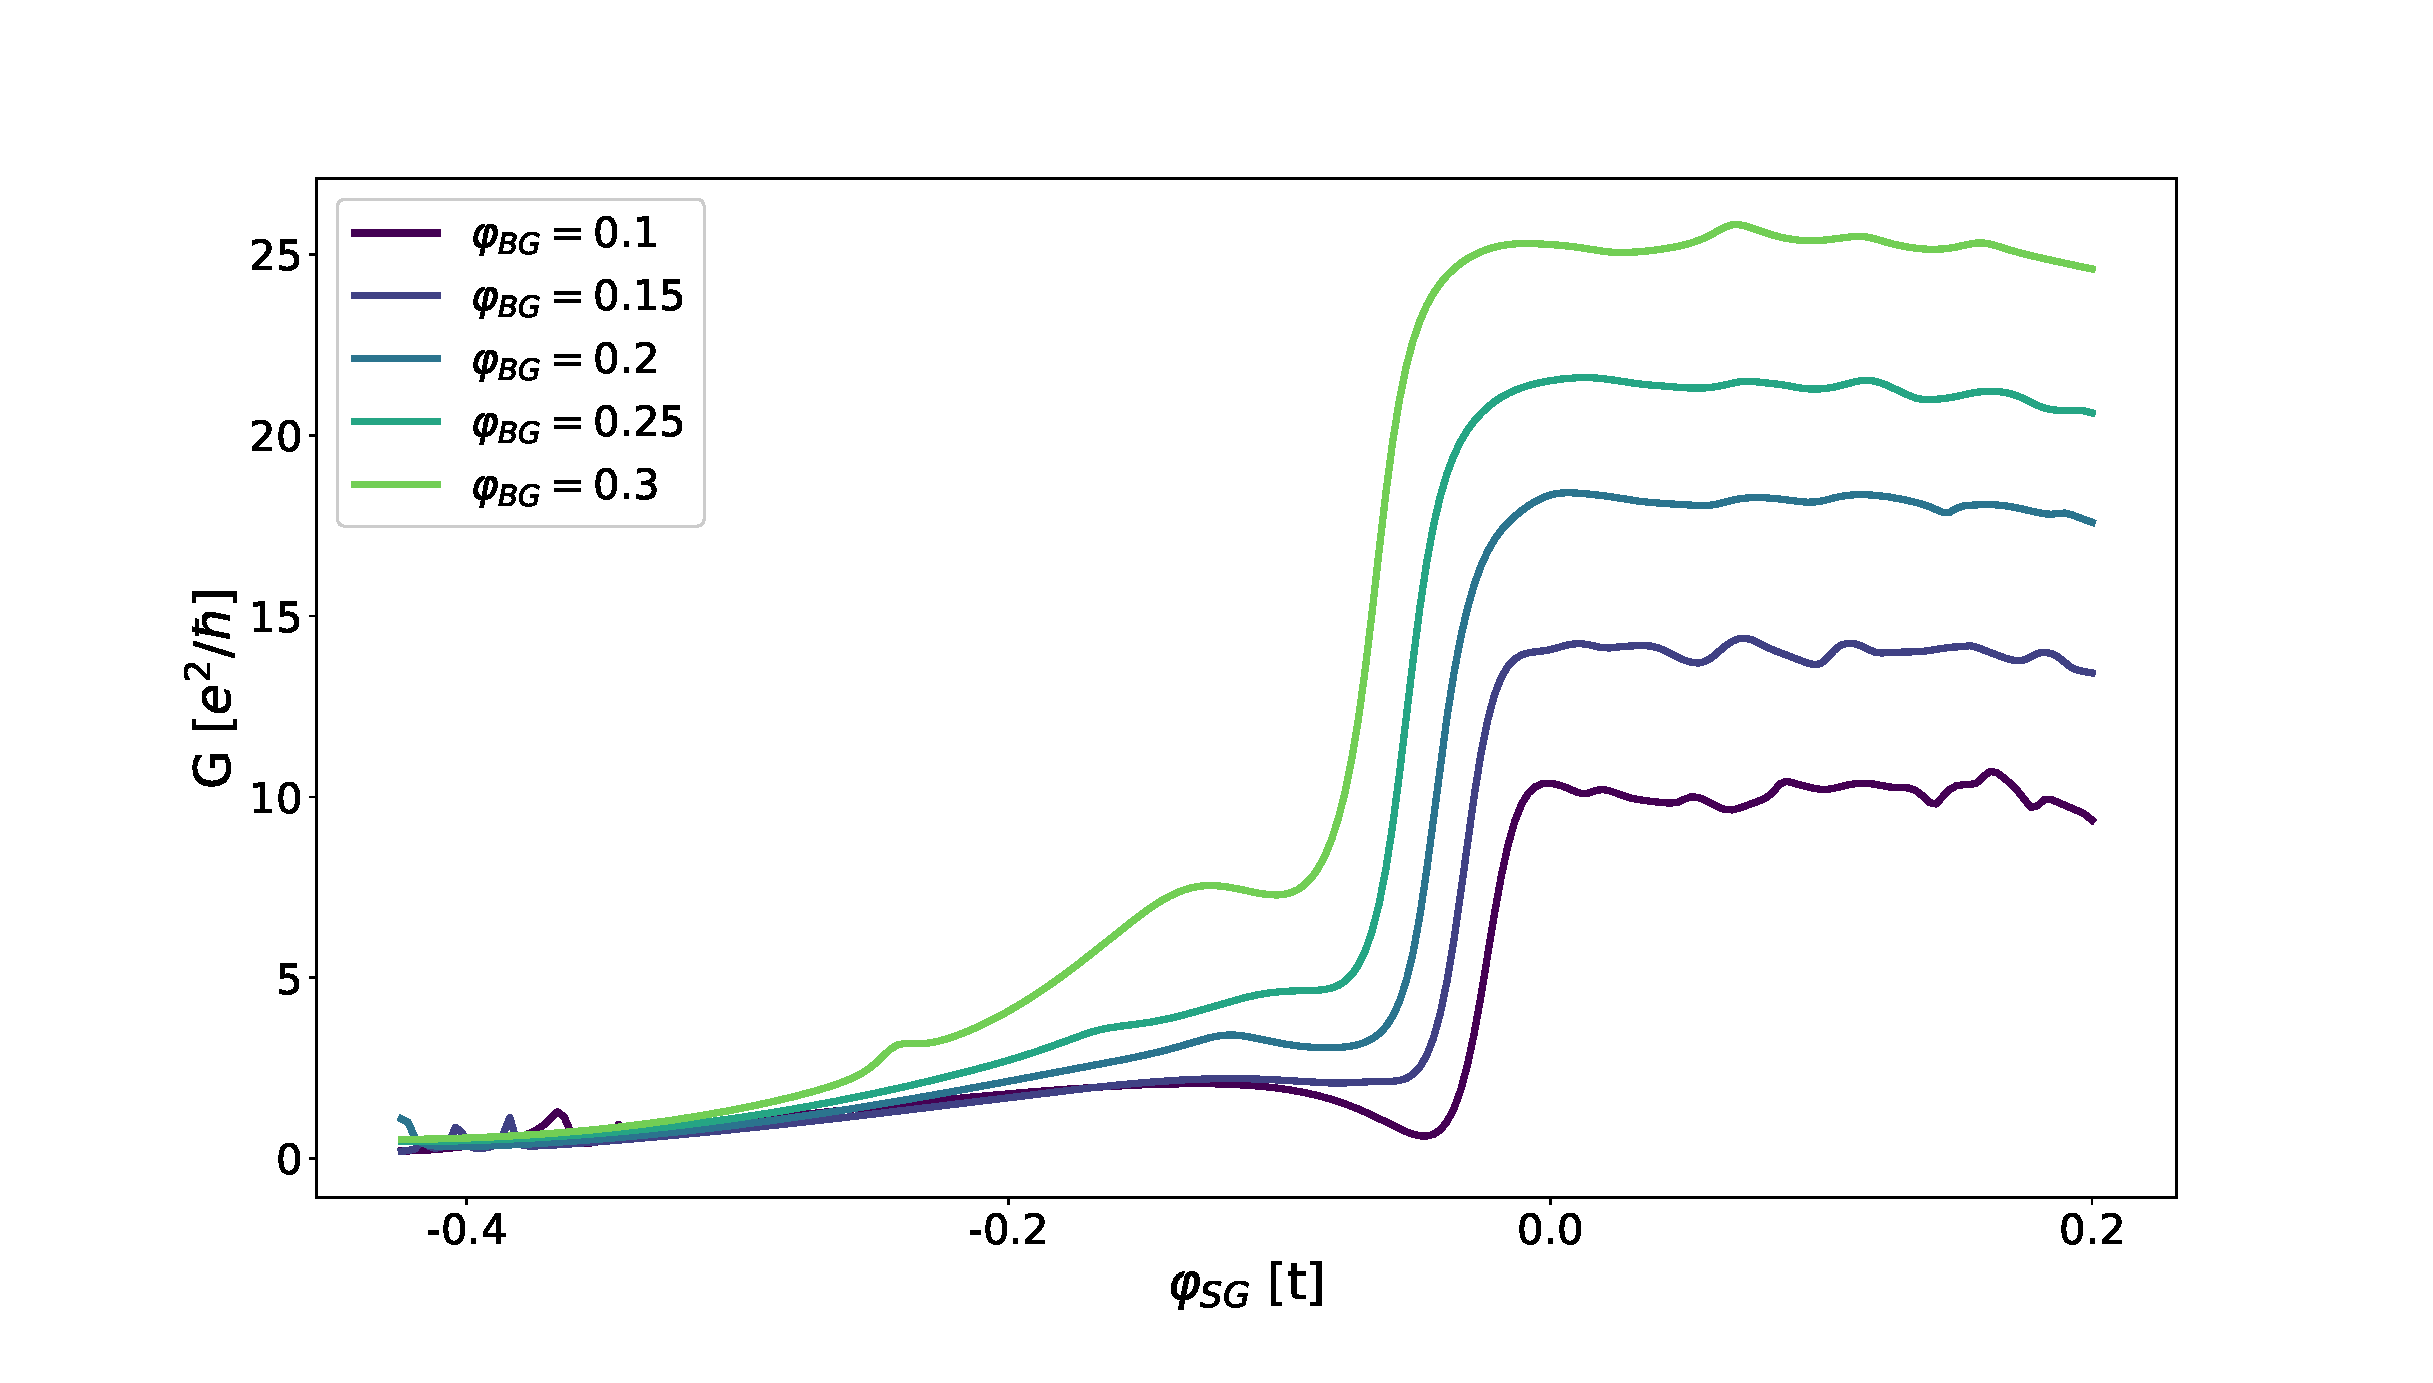
\includegraphics[width=\textwidth]{figure/numericalmodel/qpc-conductance}
%\caption{heatmap test}
%\end{figure}

\chapter{Conclusion And Outlook}
\label{ch:conclusion}
%%%%%%%%%%%%%%%%%%%%%%%%%%%%
%Zusammenfassung der Arbeit%
%%%%%%%%%%%%%%%%%%%%%%%%%%%%

%Meine Arbeit hat sich mit SNS junctions und der quasiklassischen Beschreibung beschäftigt. Ein weiterer Punkt ist die numerische Simulation von konkreten Experimenten. Ich konnte zeigen, dass die Ergebnisse von meiner


%%%%%%%%%%%%%%%%%%%%%%%%%%%%
%		Ergebnisse?		   %
%%%%%%%%%%%%%%%%%%%%%%%%%%%%
%Es wurden Ansätze für den Transport überprüft und auf den konkreten Fall des QPC übertragen (neu entwickelt, Formel). Dieser Ansatz ist anders als in Glazman, Zagoskin etc.
%Die quasiklassische Transporttheorie wurde erfolgreich auf das QPC Setup angewendet. Es konnte gezeigt werden, dass sowohl das Limit phi -> unendlich als auch phi-> 0 korrekt wiedergegeben werden. Weiterhin konnte gezeigt werden, dass das Verhalten der Kantenströme gut beschrieben werden kann.

%Auf das Experiment eingehen, was wird gut beschrieben, was nicht? Was steht 

%Eine Berechung der kritischen Stroms im Rahmen der Streumatrix-Theorie wurde implementiert. Die Tendenz ist, dass die QPC und HB Experimente richtig wiedergegeben werden. Das Waveguide Setup konnte simuliert werden, daraus konnte, weil es der tolle Fall mit translationsinvariantem System ist, die Stromdichte mit der Dyson Fuller Methode berechnet werden. 

%%%%%%%%%%%%%%%%%%%%%%%%%%%%
%		 Ausblick		   %
%%%%%%%%%%%%%%%%%%%%%%%%%%%%

%Analytische Rechnungen können für weitere Setups berechnet werden, für kompliziertere Setups. Dabei kann beispielsweise Mehrfachstreuung und Anisotrope Streeuung hinzugezogen werden. 

%Im Kontext auf die Experimente sind die Möglichkeiten beinahe unbeschränkt. Es gibt Ansätze, für Spin Orbit Coupling in BLG, die nutzen und afwändige experimentelle Setups beschreiben.





%\listoftodos
\cleardoublepage
\addcontentsline{toc}{chapter}{Bibliography}
\bibliography{literature} 

%\begin{appendix}                         %%% start the appendix for longer calculations/info
%	\chapter{Appendix}
%\end{appendix}

%\backmatter
\end{document}
